\documentclass[11pt]{article}  % Sets the font size to 12 pt and document type to article

% =============================
% Essential Packages
% =============================
\usepackage[utf8]{inputenc}     % Ensures proper encoding of special characters
\usepackage[T1]{fontenc}        % Improved font encoding
\usepackage{amsmath, amsfonts, amssymb} % Common math packages
\usepackage{geometry}           % More intuitive control over margins
\usepackage{fancyhdr}           % Custom headers and footers
\usepackage{lmodern}            % Improved Latin Modern font
%\usepackage{setspace}          % Uncomment for line spacing adjustments (e.g., \doublespacing)
\usepackage[most]{tcolorbox}
\usepackage{enumitem} 
\usepackage{hyperref}   % for clickable refs
\usepackage{cleveref}   % optional, for "Table 1" style
\usepackage{tikz}
\usepackage{listings}
\usetikzlibrary{positioning,shapes,arrows.meta,calc} % <-- added calc

\tikzset{
  block/.style={draw, rounded corners, minimum width=26mm, minimum height=7mm, align=center},
  norm/.style={draw, rounded corners, minimum width=20mm, minimum height=7mm, align=center},
  plus/.style={circle, draw, inner sep=0pt, minimum size=4mm},
}



% =============================
% Color Box
% =============================

\newtcolorbox{notebox}[2][]{%
  colback=yellow!10!white,
  colframe=yellow!50!black,
  coltitle=black,
  fonttitle=\normalfont,
  enhanced,
  attach boxed title to top left={yshift=-2mm,xshift=5mm},
  boxed title style={colback=yellow!50!white},
  title={#2},
  sharp corners=south,
  rounded corners=northwest,
  #1
}

% =============================
% Page Layout
% =============================
\geometry{
  left=1in,
  right=1in,
  top=1in,
  bottom=1in
}

% =============================
% Header Setup
% =============================
\pagestyle{fancy}
\fancyhf{}  % Clear default header/footer
\fancyhead[R]{\today}
\fancyhead[C]{LLM Handbook}
\fancyhead[L]{}
\renewcommand{\headrulewidth}{0.4pt}  % Header line thickness


% =============================
% Macros
% =============================
\usepackage{url}            % simple URL typesetting
\usepackage{booktabs}       % professional-quality tables
\usepackage{amsfonts}       % blackboard math symbols
\usepackage{nicefrac}       % compact symbols for 1/2, etc.
\usepackage{microtype}      % microtypography
%\usepackage[table]{xcolor}         % colors
\usepackage{bbm}
%\usepackage{dsfont}
\usepackage{tcolorbox}
\usepackage{euscript}    %  
\usepackage{makecell}
\usepackage{times}
\RequirePackage{fix-cm}
\usepackage{cmap}                   %   PDF
\usepackage{comment}
\usepackage{xr}
\usepackage{tikz}
%\usepackage{extsizes} %   14- 
\usepackage{csquotes} %   
\usepackage{siunitx}
\usepackage{float}
\restylefloat{table}
\usepackage{array}
%\usepackage{undertilde}
\usepackage{setspace} % 
%\onehalfspacing %  1.5
%\doublespacing %  2
%\singlespacing %  1f
\usepackage[export]{adjustbox}
\usepackage{lastpage} % ,     .
\usepackage{soulutf8} %  
\usepackage{icomma} % "" : $0,2$ --- , $0, 2$ --- 
%\newenvironment{solution}
%{\renewcommand\qedsymbol{$\blacksquare$}\begin{proof}[Solution]}{\end{proof}}
\usepackage{diagbox, eqparbox, hhline}
\usepackage{etoolbox}
\usepackage{mathtools}
\usepackage{etextools}
\usepackage{ifthen}
\usepackage{caption}
\usepackage{subcaption}
\usepackage{amsmath,amssymb, amsthm}
%\usepackage{charter}
%\usepackage{calc}
\usepackage[flushleft]{threeparttable} % http://ctan.org/pkg/threeparttable
\usepackage{calligra}
\usepackage{layout}
\usepackage{lipsum}
%\mathtoolsset{showonlyrefs=true}
\usepackage{mathrsfs}
\usepackage{color}
\usepackage{setspace}
\usepackage{multicol} %  
\usepackage{filecontents}
%nwork with tables
\usepackage{array,tabularx,tabulary,booktabs} %    
%\usepackage{longtable}  %  
\usepackage{multirow} %    
\usepackage{graphicx}
%\usepackage{subfig}
\usepackage{fancyhdr}
\usepackage{theoremref}
\usepackage{pifont}%for defining \xmark
%\usepackage[noend]{algpseudocode}
%\usepackage{verbatim}
%\usepackage[ruled,vlined]{algorithm2e}

\usepackage{algorithm}
\usepackage{algpseudocode}

\usepackage[colorinlistoftodos,bordercolor=orange,backgroundcolor=orange!20,linecolor=orange,textsize=scriptsize]{todonotes}
\usepackage{xspace}

\usepackage{hyperref}       % hyperlinks
\usepackage{cleveref}

\usepackage{enumitem}


\usepackage{wrapfig}
\usepackage{listings}
\usepackage{xcolor}
\lstdefinestyle{mystyle}{
    language=Python,
    basicstyle=\ttfamily\small,
    keywordstyle=\color{blue},
    stringstyle=\color{red},
    commentstyle=\color{gray},
    numbers=left,
    numberstyle=\tiny,
    stepnumber=1,
    breaklines=true,
    tabsize=4
}



\lstset{style=mystyle}


%%%%%%%%%%%%%%
%NEW COMMANDS   %%%
%%%%%%%%%%%%%%
\DeclareMathOperator*{\prox}{prox}
\DeclareMathOperator*{\brox}{brox}
\DeclareMathOperator*{\argmax}{arg\,max}
\DeclareMathOperator*{\argmin}{arg\,min}
\DeclareMathOperator*{\sign}{sign}
\DeclareMathOperator*{\sgn}{sgn}
\DeclarePairedDelimiter\abs{\lvert}{\rvert}

\newcommand{\inner}[2]{\left\langle #1, #2 \right\rangle}

% macros.tex

\newcommand{\mA}{\mathbf{A}}
\newcommand{\mB}{\mathbf{B}}
\newcommand{\mC}{\mathbf{C}}
\newcommand{\mD}{\mathbf{D}}
\newcommand{\mE}{\mathbf{E}}
\newcommand{\mF}{\mathbf{F}}
\newcommand{\mG}{\mathbf{G}}
\newcommand{\mH}{\mathbf{H}}
\newcommand{\mI}{\mathbf{I}}
\newcommand{\mJ}{\mathbf{J}}
\newcommand{\mK}{\mathbf{K}}
\newcommand{\mL}{\mathbf{L}}
\newcommand{\mM}{\mathbf{M}}
\newcommand{\mN}{\mathbf{N}}
\newcommand{\mO}{\mathbf{O}}
\newcommand{\mP}{\mathbf{P}}
\newcommand{\mQ}{\mathbf{Q}}
\newcommand{\mR}{\mathbf{R}}
\newcommand{\mS}{\mathbf{S}}
\newcommand{\mT}{\mathbf{T}}
\newcommand{\mU}{\mathbf{U}}
\newcommand{\mV}{\mathbf{V}}
\newcommand{\mW}{\mathbf{W}}
\newcommand{\mX}{\mathbf{X}}
\newcommand{\mY}{\mathbf{Y}}
\newcommand{\mZ}{\mathbf{Z}}

\newcommand{\ma}{\mathbf{a}}
\newcommand{\mb}{\mathbf{b}}
\newcommand{\mc}{\mathbf{c}}
\newcommand{\md}{\mathbf{d}}
\newcommand{\me}{\mathbf{e}}
\newcommand{\mf}{\mathbf{f}}
\newcommand{\mg}{\mathbf{g}}
\newcommand{\mh}{\mathbf{h}}
\newcommand{\mi}{\mathbf{i}}
\newcommand{\mj}{\mathbf{j}}
\newcommand{\mk}{\mathbf{k}}
\newcommand{\ml}{\mathbf{l}}
\newcommand{\mm}{\mathbf{m}}
\newcommand{\mn}{\mathbf{n}}
\newcommand{\mo}{\mathbf{o}}
\newcommand{\mpp}{\mathbf{p}}
\newcommand{\mq}{\mathbf{q}}
\newcommand{\mr}{\mathbf{r}}
\newcommand{\ms}{\mathbf{s}}
\newcommand{\mt}{\mathbf{t}}
\newcommand{\muu}{\mathbf{u}}
\newcommand{\mv}{\mathbf{v}}
\newcommand{\mw}{\mathbf{w}}
\newcommand{\mx}{\mathbf{x}}
\newcommand{\my}{\mathbf{y}}
\newcommand{\mz}{\mathbf{z}}


% Calligraphic letters
\newcommand{\cA}{\mathcal{A}}
\newcommand{\cB}{\mathcal{B}}
\newcommand{\cC}{\mathcal{C}}
\newcommand{\cD}{\mathcal{D}}
\newcommand{\cE}{\mathcal{E}}
\newcommand{\cF}{\mathcal{F}}
\newcommand{\cG}{\mathcal{G}}
\newcommand{\cH}{\mathcal{H}}
\newcommand{\cI}{\mathcal{I}}
\newcommand{\cJ}{\mathcal{J}}
\newcommand{\cK}{\mathcal{K}}
\newcommand{\cL}{\mathcal{L}}
\newcommand{\cM}{\mathcal{M}}
\newcommand{\cN}{\mathcal{N}}
\newcommand{\cO}{\mathcal{O}}
\newcommand{\cP}{\mathcal{P}}
\newcommand{\cQ}{\mathcal{Q}}
\newcommand{\cR}{\mathcal{R}}
\newcommand{\cS}{\mathcal{S}}
\newcommand{\cT}{\mathcal{T}}
\newcommand{\cU}{\mathcal{U}}
\newcommand{\cV}{\mathcal{V}}
\newcommand{\cW}{\mathcal{W}}
\newcommand{\cX}{\mathcal{X}}
\newcommand{\cY}{\mathcal{Y}}
\newcommand{\cZ}{\mathcal{Z}}

% Bracket macros
\newcommand{\cbrac}[1]{\left\{ #1 \right\}}   % Curly braces
\newcommand{\sbrac}[1]{\left[ #1 \right]}     % Square brackets
\newcommand{\rbrac}[1]{\left( #1 \right)}     % Round parentheses
% Norm macro
\newcommand{\norm}[1]{\left\lVert #1 \right\rVert}
\newcommand{\normsub}[2]{\left\lVert #1 \right\rVert_{#2}}
\newcommand{\normarrow}[3]{\left\lVert #1 \right\rVert_{#2 \rightarrow #3}}
\newcommand{\normabs}[1]{\left\lvert #1 \right\rvert}


\let\la=\langle
\let\ra=\rangle

\def\<{\left\langle}
\def\>{\right\rangle}
% \def\[{\left[}
%\def\]{\right]}
\def\({\left(}
\def\){\right)}

%\newcommand{\st}{\;:\;}
\newcommand{\ve}[2]{\langle #1 ,  #2 \rangle}

%\newcommand{\eqdef}{\stackrel{\text{def}}{=}}
\newcommand{\eqdef}{:=}
\newcommand{\ii}{{}^{(i)}}


\newcommand{\Prob}{\mathbf{Prob}}
\newcommand{\E}{\mathbf{E}}
\newcommand{\R}{\mathbb{R}}
\newcommand{\N}{\mathbb{N}}


% sets
\DeclareMathOperator{\card}{card}       % cardinality of a set
\DeclareMathOperator{\diam}{diam}       % diameter of a set
\DeclareMathOperator{\MVEE}{MVEE}       % minim volume enclosing ellipsoid of a set
\DeclareMathOperator{\vol}{vol}         % volume of a set

% statistical
% \DeclareMathOperator{\Exp}{{\rm E}}           % expectation
%\newcommand{\Exp}[1]{{\rm E}\left[#1\right]}
\newcommand{\Exp}[1]{\mathbb{E}\left[#1\right]}
\newcommand{\Expu}[2]{\mathbb{E}_{#1}\left[#2\right]}
\newcommand{\ExpSub}[2]{\mathbb{E}_{#1}\left[#2\right]}
% Trace macro
\newcommand{\tr}[1]{\mathrm{tr}\left(#1\right)}


\DeclareMathOperator{\Cov}{Cov}         % covariance
\DeclareMathOperator{\Var}{Var}         % variance
\DeclareMathOperator{\Corr}{Corr}       % correlation
\DeclareMathOperator{\LMO}{LMO} 

% functions and operators
\DeclareMathOperator{\signum}{sign}     % signum/sign of a scalar
\DeclareMathOperator{\dom}{dom}         % domain
\DeclareMathOperator{\epi}{epi}         % epigraph
\DeclareMathOperator{\Ker}{null}        % nullspace/kernel
\DeclareMathOperator{\nullspace}{null}  % nullpsace
\DeclareMathOperator{\range}{range}     % range
\DeclareMathOperator{\Image}{Im}        % image

% topology
\DeclareMathOperator{\interior}{int}    % interior
\DeclareMathOperator{\ri}{rint}         % relative interior
\DeclareMathOperator{\rint}{rint}       % relative interior
\DeclareMathOperator{\bdry}{bdry}       % boundary
\DeclareMathOperator{\cl}{cl}           % closure

% vectors, matrices
\DeclareMathOperator{\linspan}{span}
\DeclareMathOperator{\linspace}{linspace}
\DeclareMathOperator{\cone}{cone}

%\DeclareMathOperator{\tr}{tr}           % trace
\DeclareMathOperator{\rank}{rank}       % rank
\DeclareMathOperator{\conv}{conv}       % convex hull
\DeclareMathOperator{\Diag}{Diag}       % Diag(v) = diagonal matrix with v_i on the diagonal
\DeclareMathOperator{\diag}{diag}       % diag(D) = the diagonal vector of matrix D

\DeclareMathOperator{\Arg}{Arg}         % Argument




\newtheorem{theorem}{Theorem}
\newtheorem{proposition}{Proposition}

\theoremstyle{plain}

\newtheorem{example}{Example}
\newtheorem{assumption}{Assumption}
\newtheorem{lemma}{Lemma}
\newtheorem{fact}{Fact}

\newtheorem{prop}[theorem]{Proposition}
\newtheorem{corollary}{Corollary}
\newtheorem{lem}[theorem]{Lemma}
\newtheorem{claim}[theorem]{Claim}
\newtheorem{remark}{Remark}


\newtheorem{exercise}[theorem]{Exercise}

\newtheorem{rem}[theorem]{Remark}
\newtheorem{que}[theorem]{Question}
\newtheorem{definition}{Definition}


%zerosarah paper symbols

\newcommand*{\qedb}{\hfill\ensuremath{\square}}   % or \blacksquare
\newcommand{\topic}[1]{\vspace{2mm}\noindent{{\bf #1:}}}
\newcommand{\head}[1]{\noindent{{\bf #1:}}}

\definecolor{mydarkgreen}{RGB}{39,130,67}
\definecolor{mydarkred}{RGB}{192,47,25}
\definecolor{mydarkblue}{RGB}{39,47,180}
\definecolor{mydarkpurple}{RGB}{48,25,52}
\newcommand{\green}{\color{mydarkgreen}}
\newcommand{\red}{\color{mydarkred}}
\newcommand{\blue}{\color{mydarkblue}}
\newcommand{\purple}{\color{mydarkpurple}}

\newcommand{\zerosarah}{{\sf ZeroSARAH}\xspace}
\newcommand{\clip}{\operatorname{clip}}



\definecolor{lightblue}{RGB}{224, 240, 255} % Adjust RGB values as needed
\definecolor{bgcolor}{rgb}{0.8,1,1}
\definecolor{bgcolor2}{rgb}{0.8,1,0.8}
\newenvironment{proofof}[1]{\smallskip\noindent{\bf \em Proof of #1.}}%





\newcommand{\peter}[1]{\todo[inline]{\textbf{Peter: }#1}}
\newcommand{\igor}[1]{\todo[inline]{\textbf{Igor: }#1}}
\newcommand{\abdurakhmon}[1]{\todo[inline]{\textbf{Abdurakhmon: }#1}}
\newcommand{\hanmin}[1]{\todo[inline]{\textbf{Hanmin: }#1}}

\newcommand{\algname}[1]{{\sf \footnotesize \color{mydarkgreen} #1}\xspace}

%\newcommand{\theHalgorithm}{\arabic{algorithm}}


\newcommand{\rA}{{\red A}}
\newcommand{\rB}{{\red B}}

\newcommand{\dmodel}{d_{\text{model}}}
\newcommand{\dhead}{d_{\text{head}}}
\newcommand{\RBLDh}{\R^{B \times L \times \dhead}}
\newcommand{\RBLDm}{\R^{B \times L \times \dmodel}}
\newcommand{\RBLE}{\R^{B \times L \times E}}
\newcommand{\softmax}{\text{softmax}}
\newcommand{\floor}[1]{\left\lfloor #1 \right\rfloor}
\newcommand{\boxtext}[1]{\boxed{\text{#1}}}
\newcommand{\prob}[1]{\mathbb{P}\rbrac{#1}}
\newcommand{\probsub}[2]{\mathbb{P}_{#1}\rbrac{#2}}
\newcommand{\din}{d_{\text{in}}}
\newcommand{\dout}{d_{\text{out}}}
\newcommand{\klD}[2]{{\rm D}_{\text{KL}}\rbrac{#1 \parallel #2}}
\newcommand{\pisub}[3]{\pi_{#1}\rbrac{#2 \mid #3}}
\newcommand{\thetaold}{\theta_{\text{old}}}
\newcommand{\thetaref}{\theta_{\text{ref}}}  % No .tex extension needed


% =============================
% Begin Document
% =============================
\begin{document}

\tableofcontents

\section{Linear Algebra}


\subsection{Column wise decomposition.}
Any matrix $\mA \in \R^{m \times n}$ can be decomposed into the sum of its columns: 
\begin{align}
	\mA = \sum_{i=1}^{n} \mA_{:j} e_j^{\top},
\end{align}
where $e_j$ are standard basis vectors of $\R^n$.
Notice that this is a rank $1$ decomposition.

\subsection{Row wise decomposition.}
Any matrix $\mA \in \R^{m \times n}$ can be decomposed into the sum of its rows: 
\begin{align}
	\mA = \sum_{i=1}^{m} e_i \mA_{i:}^{\top},
\end{align}
where $e_i$ are standard basis vectors of $\R^m$.
Notice that this is a rank $1$ decomposition.


\section{Multithreading}
Per-thread scratch buffers (aka thread-local workspaces) are a very common pattern to cut allocation overhead and lock contention in multi-threaded code.
In this way we do not create lots of short-lived temporaries, and have better cache locality and to avoid false sharing on shared buffers.


\section{LLM Training}
\subsection{Scaling the logits after LLM head.}
We usually apply RMS norm to normalize (along the last dimension $E$, where it stands for model dimension, $B$ means batch size and $L$ means sequence length) the tensor $\mX \in \R^{B \times L \times E}$ we feed into LLM head, and obtain the corresponding logits $l$.
After RMS normalization, each tensor corresponding to the token $x_i \in \R^E$ will then have ${\rm RMS}(x_t) = 1$.
Now notice that for each coordinate $x_{i, t}, t\in[E]$, treating as a random variable, its variance is given by 
\begin{align}
  \Var\rbrac{x_{i, t}} = \Exp{x^2_{i, t}} - \rbrac{\Exp{x_{i, t}}}^2,
\end{align}
and if it is zero-mean (or small), then $\Var\rbrac{x_{i, t}} \simeq \Exp{x^2_{i, t}}$, which is to say that second moment reflects the variance.

The next step is to use the empirical observation that for linear layers, hidden vectors tend to be approximatedly rotation-invariant (isotropic), i.e., each coordinate behaves like the others, so we can use the second moment over the coordinate in a token to replace the actual second moment.
And the former, is given by 
\begin{align}
  \Var\rbrac{x_{i, t}} \simeq \frac{1}{E}\sum_{t=1}^{E}x_{i, t} = 1.
\end{align}
Now we start to consider the logits, which is generated by 
\begin{align*}
  l_{j, i} = w_j^{\top}x_i = \sum_{t=1}^{E}w_{j, t}x_{i, t}.
\end{align*}
If we assume each weight entry $w_{j, t}$ are i.i.d. with variance $\sigma^2$ the logits variance is give by 
\begin{align*}
  \Var\rbrac{l_{j, i}} = \sum_{t=1}^{E} \sigma^2 \Var \rbrac{x_{t, i}} \simeq E \sigma^2.
\end{align*}
So the standard deviation $\sim \sqrt{E}$.
To ensure that logits do not scale with the model dimension, we scale it by $\sqrt{E}$.



\section{Attention}

\subsection{Multihead Self Attention (MHA)}
Consider an input tensor $\mX \in \R^{B \times L \times d_{\text{model}}}$ to an attention layer, where $B$ is the batch size, $L$ is the sequence length, and $d_{\text{model}}$ is the model dimension.

\begin{enumerate}
  \item The first step involves computing queries, keys, and values. 
  We have three matrices, $\mW_q$, $\mW_k$, and $\mW_v \in \R^{d_{\text{model}} \times d_{\text{model}}}$, and simultaneously perform the following operations
  \begin{align}
    \mQ = \mX \mW_{q};\quad \mK = \mX \mW_{k};\quad \mV = \mX\mW_{v}.
  \end{align}
  These operations are vectorized, meaning that for each sequence $b$ in the batch of size B, we do 
  \begin{align*}
    \mQ_b = \mX_b\mW_{q} \quad \forall b \in [B].
  \end{align*} 
  $\mW_q$, $\mW_k$, and $\mW_v$ are trainable parameters shared across the entire batch. 
  The resulting $\mQ$, $\mK$, and $\mV$ have the shape $\R^{B \times L \times d_{\text{model}}}$.

  \item Next, for multihead attention, we reshape $\mQ$, $\mK$, and $\mV$ from shape $\R^{B \times L \times d_{\text{model}}}$ into $\R^{B \times H \times L \times d_{\text{head}}}$, where $H$ is the number of attention heads and $d_{\text{head}}$ is the dimension of each head.
  To achieve this, we first divide $d_{\text{model}}$ into $H$ heads, resulting in shapes of $\R^{B \times L \times H \times d_{\text{head}}}$. 
  Then we rearrange into $\R^{B \times H \times L \times d_{\text{head}}}$.
  Conceptually, each head uses a subset of dimensions from $d_{\text{model}}$ to compute scores between queries and keys along the sequence dimension $L$.
  We will use the following notations $\mQ_h, \mK_h, \mV_h$ to denote the per head tensor in $R^{B \times 1 \times L \times d_{\text{head}}}$ for each head $h \in [H]$.

  \item In the next step, we perform the attention calculation:
  \begin{align*}
    \mS_h &\eqdef \text{Scores}_h(\mQ_h, \mK_h) = \frac{\mQ_h \mK_h^{\top}}{\sqrt{d_{\text{head}}}} + \mM\\
    \mA_h &\eqdef \text{Attention}_h(\mQ, \mK, \mV) = \text{softmax}\rbrac{\mS_h}\mV_h, \quad \forall h \in [H].
  \end{align*}
  The scaled multiplication of $\mQ_h$ and $\mK^{\top}_h$ is vectorized, resulting in $\mS_h \in \R^{B\times 1\times L \times L}$ and $\mS \in \R^{B\times H\times L \times L}$.\footnote{Here $\mS$ is the stack of $\mS_h$ along dimension $H$.}
  Optionally, we could use a mask matrix to mask out certain tokens, an example would be the causual self attention.
  To stabilize the gradients, we element-wise divide raw scores by $\sqrt{d_{\text{head}}}$.
  This scaling choice can be justified because each element of $\mQ_h\mK_h^{\top}$ represents a dot product between vectors of dimension $d_{\text{model}}$. 
  The variance of this dot product scales as $\Var\rbrac{\inner{q_h}{k_h}}\sim d_{\text{model}}\sigma_q^2\sigma_k^2$. 
  Since variance scales quadratically, we divide by $\sqrt{d_{\text{head}}}$.
  The softmax operation turns the scores after masking into probabilities, along the last dimension.\footnote{This is to say that for each $L \times L$ matrix, we softmax every row.}
  Imagine $z = [z_1, \hdots, z_L] \in \R^L$ is a row vector, then essentially, softmax defines the operation:
  \begin{align}
    \sigma(z)_i \eqdef \frac{e^{z_i}}{\sum_{j=1}^{L}e^{z_j}}.
  \end{align}
  Sometimes we use a numerically stable version to replace it 
  \begin{align}
    \tilde{\sigma}(z) \eqdef \frac{e^{z_i - \max(z)}}{\sum_{j=1}^{L}e^{z_j - \max(z)}}.
  \end{align}

  It is worth mentioning that in single head attention (scaled dot product), the complexity of computation is $\cO\rbrac{BL^2d_{\text{model}}}$, while for multihead attention, it is the same since we do $\cO\rbrac{H \times BL^2d_{\text{head}}} = \cO\rbrac{BL^2d_{\text{model}}}$. 

  \item Finally, we concatenate and mix attention outputs from all heads. 
  Concatenation involves first transposing $\mA_h$ to $\R^{B \times L \times H \times d_{\text{head}}}$ and then merging the last two dimensions into $\mA \in \R^{B \times L \times d_{\text{model}}}$. 
  This concatenated result is projected using a matrix $\mW_O$, as follows:
  \begin{align}
    \text{MHA}(\mX) = \mA\mW_{O}. 
  \end{align}
  The final output retains the shape $\R^{B \times L \times d_{\text{model}}}$.
\end{enumerate}
There a bunch of reasons why we are using multi heads instead of scaled dot product attention. 
\begin{itemize}
  \item \textbf{Diversity of learned attention patterns}: Each head learns different attention patterns in parallel. 
  A single attention head computes only one set of attention scores.

  \item \textbf{Subspace specialization}: Instead of operating in $d_{\text{model}}$, each head projects to a lower dimension subspace $d_{\text{head}}$.
  This suggests that each head operates in a distinct feature subspace.

  \item \textbf{Improved gradient flow and representation mixing}: Independent paths improve gradient flow and richness of learned representations.
\end{itemize}
Notice that the computational cost are the \textbf{SAME}!

\subsection{Multi Query Attention (MQA)}
In MQA, different heads have its own query, but share the same key and value.
Specifically, for a head $h$, we have 
\begin{align*}
  \mS_h &\eqdef \text{Scores}(\mQ_h, \mK) = \frac{\mQ_h\mK^{\top}}{\sqrt{d_{\text{head}}}} + \mM \\
  \mA_h &\eqdef \text{Attention}_h (\mQ_h, \mK, \mV) = \text{softmax}(\mS_h)\mV, \quad \forall h \in [H]. 
\end{align*}
This means that for each head $h$, we have a separate $\mQ_h \in \R^{B \times 1 \times L \times d_{\text{head}}}$ and shared $\mK, \mV \in \R^{B \times 1 \times L \times d_{\text{head}}}$.

Compared to standrad MHA, MQA has the following features:
\begin{itemize}
  \item \textbf{Reduced parameter count}: Each head has its own query only, shared key and value.
  \item \textbf{Smaller activation size (memory usage)}: Now $\mK, \mV \in \R^{B \times 1 \times L \times d_{\text{head}}}$, so the activation size is smaller.
  \item \textbf{Reduced KV cache (fast inferencing)}: For transformer based models such as GPT, we generate text one token at a time. 
  To avoid recomputing attention over all previous tokens on every step, we cache $k, v$ (key and value vectors) for all previously seen tokens.
  Specifically, in standard MHA, for each layer and token generated, we neeed $2BHLd_{\text{head}}$ for cached $\mK, \mV$.
  In MQA, we share $\mK$ and $\mV$ so that the cost becomes $2BLd_{\text{head}}$.
  \item \textbf{Minimal accuracy loss.} Used in GPT-3.5, PaLM, LLaMA, etc.
\end{itemize}

\subsection{KV cache}
The motivation for KV caching is to enable efficient inference — both in terms of compute time and memory bandwidth.
At inference time only, autoregressive models input a sequence of tokens $\cbrac{x_t, \hdots, x_{t + L - 1}}$ to generate the next token $x_{t + L}$. 
To avoid recomputing key and value vectors for all previous tokens every time, we cache the $k, v$ pairs corresponding to the tokens $x_t \hdots, x_{t + L - 1}$ in the forward pass.
Then, when generating $x_{t + L + 1}$, we can reuse the vectors for cached $x_{t + 1}, \hdots, x_{t + L - 1}$ and we only need to compute $k, v$ for $x_{t + L}$. 
This mechanism is known as the \textbf{KV cache}.


\subsection{Grouped Query Attention (GQA)}
GQA is like an interpolation between MQA and MHA, where we ask groups of heads to share $\mK, \mV$.
Specifically, let $g(h)$ be a function that maps a head $h$ to its corrsponding group index, then we have 
\begin{align*}
  \mS_h &\eqdef \text{Scores}(\mQ_h, \mK_{g(h)}) = \frac{\mQ_h\mK^{\top}_{g(h)}}{\sqrt{d_{\text{head}}}} + \mM \\
  \mA_h &\eqdef \text{Attention}_h (\mQ_h, \mK_{g(h)}, \mV_{g(h)}) = \text{softmax}(\mS_h)\mV_{g(h)}, \quad \forall h \in [H]. 
\end{align*} 
Benefits:
\begin{enumerate}
  \item Less memory than MHA.
  \item Flexible compute/memory tradeoff by controlling the number of k, v heads.
\end{enumerate}
It is used in LLaMA 2 and Mistral.



\subsection{Multihead Latent Attention (MLA)}
Before we go into details, we need to first differentiate between self attention and cross attention. 
\begin{itemize}
  \item Self attention is the case when Q, K, V comes from the same input sequence. Its typically used in encoder blocks of BERT, GPT, LLaMA, etc, and decoder blocks in GPT, T5, etc.
  \item Cross attention refers to the case when Q comes from one sequence but K, V comes from another sequence. It is typically used in the case that decoder attends to encoder outputs (T5, BART), and the case of vision language models where text attends to image, and perceiver-style latent attention.
\end{itemize}
We can formulate cross attention in the following way: Let $\mZ \in \R^{B \times M \times d_{\text{model}}}$ (expanded from $\R^{1 \times M \times d_{\text{model}}}$.) be a target sequence (queries) and $\mX \in \R^{B \times L \times d_{\text{model}}}$ be a source sequence (keys and values),
\begin{align}
  \mQ = \mZ\mW_q; \quad \mK = \mX\mW_k; \quad \mV = \mX\mW_v.
\end{align}
Notice that $M$ could be different than $L$.
In the case of cross-attention with a latent array, we often have, $M << L$, which significantly reduces computational cost by avoiding full self-attention over the entire input sequence.
We then compute the attention scores and softmax:
\begin{align}
  \mS_h &\eqdef \text{Scores}(\mQ_h, \mK_{h}) = \frac{\mQ_h\mK^{\top}_{h}}{\sqrt{d_{\text{head}}}} \\
  \mA_h &\eqdef \text{Attention}_h (\mQ_h, \mK_{h}, \mV_{h}) = \text{softmax}(\mS_h)\mV_{h}, \quad \forall h \in [H].
\end{align}
Notice that in this case $\mS_h \in \R^{B \times 1 \times M \times L}$ and $\mA_h \in \R^{B \times 1 \times M \times d_{\text{head}}}$ for head $h \in [H]$. 
After concatenation, we result in $\mA \in \R^{B, M \times d_{\text{model}}}$, which is like we are focusing on a smaller sequence.
In MLA, latent vector it self is a learnable parameter and shared accross a batch. 
These latents act like information bottleneck that extract useful features from the long input $\mX \in \R^{B \times L \times d_{\text{model}}}$.



\subsection{Latent Transformer Block}
This is a key design of Perceiver (2021, DeepMind), Set Transformer and efficient transformers for long inputs (e.g., audio, video, documents).
Essentially it can be viewed as cross attention followed by latent self-attention.
Mathematically speaking, we are giving a vector $\mX \in \R^{B \times L \times d_{\text{model}}}$. 
First we are using the latent vector $\mZ \in \R^{1 \times M \times d_{\text{model}}}$ (expanded accross batch dimension.) and the input $\mX \in \R^{B \times L \times d_{\text{model}}}$, we have 
\begin{align*}
  \mA_1 = \text{Attention}(\mX_q = \mZ, \mX_k = \mX, \mX_v = \mX),
\end{align*}
which essentially asks "What should I learn from all of you tokens?".
After this step: each latent now contains information extracted from the input.
Notice that now $\mA_1 \in \R^{B \times M \times d_{\text{model}}}$ is a compressed representation of $\mX$, extracted by the latent array.
Then we do normal self attention on the latent variable:
\begin{align*}
  \mA_2 = \text{Attention}(\mX_q = \mA_1, \mX_k = \mA_1, \mX_v = \mA_1)
\end{align*}
where each latent vector is allowed to look at other latents, share what they learned and refine itself.
\begin{verbatim}
  for each block:
    z = z + CrossAttention(q ← z, k ← x, v ← x)
    z = z + SelfAttention(q ← z, k ← z, v ← z)    
\end{verbatim}
Before we actually feed the $\mZ$ and $\mX$ into the attention block and the final feed forward layer, we first do normlization (LayerNorm in the case of my code).



\subsection{Pre- and Post- Normlization}
In general, there are two ways of doing layer normlization, Post-LN and Pre-LN. 
In the original implementation of transformer, post-LN is used. 
However, pre-LN has become the modern default, which is used in GPT-2/3/4, T5, LLaMA, PaLM, Perceiver, etc.
The benefits of using pre-LN includes the follows:
\begin{itemize}
  \item {\bf (Help gradient flow \& increasing training stability)}: In a deep stack, residual paths carry the untouched signal forward. 
  With Pre-LN, those residual paths also carry unit-variance, zero-mean activations (because they are already normalized). 
  That keeps gradients well-scaled and prevents the exploding / vanishing issues that appeared when stacking 24 - 100+ layers with Post-LN.
  Empirically, Pre-LN lets you train hundreds (even thousands) of layers with a stable learning rate schedule, whereas Post-LN often needed warm-up tricks or gradient clipping.
  \item {\bf (Easier optimization of very long sequences)}: Cross-entropy loss is applied after the final LayerNorm.
  With Post-LN every sub-layer's output is renormalized, the network must constantly “undo” those shifts.
  Pre-LN leaves the residual branch untouched, so the model can accumulate information across time steps or tokens without repeatedly rescaling it.
  \item {\bf (Faster convergence)}: Many ablations show ~ 1.3 - 1.5x faster convergence for GPT/T5 style models when switching from Post-LN → Pre-LN. This is because every tensor that flows straight down the stack (both forward activations and backward gradients through the residual skip) has mean 0 and variance 1, which helps stabilize second-moment estimate quickly for Adam.
  \item {\bf (Safer with half-precision / mixed-precision)}: Normalizing before the high-variance matrix multiplications keeps activations in a narrower numeric range, reducing overflow/underflow risk in FP16/BF16 training.
\end{itemize}


\textbf{LayerNorm:} Mathematically speaking, consider an input $\mX$ in the space $\R^{B \times L \times d_{\text{model}}}$, for the $l$-th token in the $b$-th batch
\begin{align*}
  \mL[b, l, :] = \text{LayerNorm}(\mX[b, l, :]) = \gamma \cdot \frac{X[b, l, :] - \mu_{n, l}}{\sqrt{\sigma^2_{b, l}} + \epsilon} + \beta, 
\end{align*}
where 
\begin{align*}
  \mu_{b, l} = \frac{1}{d_{\text{model}}}\sum_{i=1}^{d_{\text{model}}}\mX[b, l, i], \quad \sigma^2_{b, l} = \frac{1}{d_{\text{model}}}\sum_{i=1}^{d_{\text{model}}}\rbrac{\mX[b, l, i] - \mu_{b, l}}^2,
\end{align*}
$\gamma, \beta \in \R^{d_{\text{model}}}$ are learned shift and scale vectors.
Notice that statistics are computed per sample, per position, no batch coupling, so the network behaves the same in training and inference and is robust to batch-size 1. 
Its benefits includes: 
\begin{itemize}
  \item {\bf (Zero-mean, unit-var features).} Keeps dot-products in a predictable range, resulting in stable softmax gradients.
  \item {\bf (Identical behaviour in training / inferencing).} Important for autoregressive generation where batch size changes.
  \item {\bf (Works with any sequence length).} No running-average statistics needed.
\end{itemize}
In a simpler form, layernorm can be written as 
\begin{align*}
  \mL = \gamma \odot \frac{\mX - \mu}{\sqrt{\sigma + \epsilon}} + \beta,
\end{align*}
where all operations are elementwise.
Notice that $\gamma, \beta \in \R^{d_{\text{model}}}$ are learnable parameters.


\subsection{Dropout}
\paragraph{During Training:}
This refers to During training we randomly set a fraction of the sub-layer output activations to zero and scale the survivors.
Specifically, for $\mX \in \R^{B \times L \times d_{\text{model}}}$ and the drop out rate $0 < p < 1$, we sample a binary traning mask $\mM \in \cbrac{0, 1}^{B \times L \times d_{\text{model}}}$, using the Bernoulli($q$) distribution where $q = 1 - p$, we then apply 
\begin{align*}
  \widehat{\mX} = \frac{1}{q}\mX \odot \mM.
\end{align*}
$q$ is referred to as the keep probability, and we are trying to make $\Exp{\widehat{\mX}} = \mX$.
\paragraph{During Inferencing:}
At inference time the mask is removed and $\mX$ passes through unchanged. Code: 
\begin{verbatim}
  torch.nn.Dropout(p=p)
\end{verbatim}

\subsection{DCA}
This one seems to be less well known, on medical image tasks.

\subsection{Linear Attention}
Let us first look at the asymptotic time complexity and memory complexity of attention.
\begin{table}[H]
\label{table1}
\centering
\renewcommand{\arraystretch}{1.2}
\begin{tabular}{@{}l c@{}}
\toprule
\textbf{Operation} & \textbf{Complexity} \\
\midrule
Projections $\mX \mapsto (\mQ,\mK,\mV)$ & $\cO\left(BLd_{\text{model}}^{2}\right)$ \\
Score computation $\mQ\mK^{\top}$ (per head) & $\cO\left(BHL^{2}\dhead\right)$ \\
Softmax over scores & $\cO\left(BHL^{2}\right)$ \\
Weighted sum $\mathrm{softmax}(\mQ\mK^{\top})\mV$ & $\cO\left(BHL^{2}\dhead\right)$ \\
Output projection (concat heads $\to d_{\text{model}}$) & $\cO\left(BLd_{\text{model}}^{2}\right)$ \\
\bottomrule
\end{tabular}
\caption{Computation complexity of the main steps in a standard self-attention block. 
Here $B$ = batch size, $L$ = sequence length, $H$ = number of heads, $\dhead$ = head dimension, and $d_{\text{model}} = H \cdot \dhead$.}
\end{table}
For naive self-attention, we can see that as sequence length becomes longer, the dominating term would be $\cO(BHL^2\dhead)$, which becomes $\cO(BHL_qL_k\dhead)$, which is quadratic in $L$.

\paragraph{Memory consumption:} 
\begin{itemize}
  \item Store $\mQ, \mK$ and $\mV$: $\cO(BL\dmodel)$
  \item Store attention scores/probs: $\cO(BHL^2)$
  \item Output activations for backprob add similar terms.
  \item By FlashAttention / PyTorch SDPA (streaming): we keep compute the same $\cO(BHL^2\dhead)$ but reduce memory from $\cO(BHL^2)$ to roughly $\cO(BL\dmodel)$ by not materializing the full $L \times L$ matrix. 
\end{itemize}

\begin{table}[h]
\centering
\renewcommand{\arraystretch}{1.2}
\begin{tabular}{@{}lcc@{}}
\toprule
\textbf{Scenario} & \textbf{Time (leading term)} & \textbf{Memory (leading term)} \\
\midrule
Self-attention (train) & $O\!\left(BHL^{2}d_{\text{head}}\right)$ & $O\!\left(BHL^{2}\right)$ \\
Cross-attention & $O\!\left(BHL_{q}L_{k}d_{\text{head}}\right)$ & $O\!\left(BHL_{q}L_{k}\right)$ \\
With FlashAttention / SDPA & same time & $O\!\left(BLd_{\text{model}}\right)$ \\
Autoregressive decoding (per token at step $t$) & $O\!\left(Htd_{\text{head}}\right)$ & cache $O\!\left(Ld_{\text{model}}\right)$ \\
\bottomrule
\end{tabular}
\caption{Asymptotic compute and memory complexity for different attention scenarios. 
Here $B$ = batch size, $L$ = sequence length (train), $H$ = number of heads, $d_{\text{head}}$ = per-head dimension, $d_{\text{model}} = H \cdot d_{\text{head}}$, $L_q$/$L_k$ = query/key lengths for cross-attention, and $t$ = current decoding step in autoregressive inference. Autoregressive decoding is with KV cache.}
\end{table}

\paragraph{Linear attention:} The linear attention is introduced to avoid the quadratic dependence using attention kernels which allow us to obtain linear dependence. 
Note that the attention of token $i$ is given by 
\begin{align*}
  \text{attn}_i = \frac{\sum_{j=1}^{L}\exp\rbrac{\frac{\mq_i^{\top}\mk_j}{\sqrt{\dhead}}}\mv_j}{\sum_{j=1}^{L}\exp\rbrac{\frac{\mq_i^{\top}\mk_j}{\sqrt{\dhead}}}}.
\end{align*}
To compute it, we need to perform $\mQ\mK^{\top}$ and apply softmax rowwise.
We introduce the kernel trick just as we did in SVM, imagine we can write 
\begin{align*}
  \exp\rbrac{\frac{\mq_i^{\top}\mk_j}{\sqrt{\dhead}}} \approx \phi(\mq_i)^{\top} \phi(\mk_j),
\end{align*}
for some feature map $\phi: \R^{\dhead} \mapsto \R^{d_{\phi}}$ with non-negative outputs, then we have
\begin{eqnarray*}
  \text{Numerator:} \qquad && \sum_{j=1}^{L} \phi(\mq_i)^{\top}\phi(\mk_j) \mv_j^{\top} = \rbrac{\sum_{j=1}^{L}\mv_j\phi(\mk_j)^{\top}} \cdot \phi(\mq_i), \\
  \text{Denominator:} \qquad && \sum_{j=1}^{L} \phi(\mq_i)^{\top}\phi(\mk_j) = \rbrac{\sum_{j=1}^{L}\phi(\mk_j)^{\top}} \cdot \phi(\mq_i).
\end{eqnarray*}
Now denote $\mS_\mV \eqdef \sum_{j=1}^{L}\mv_j\phi(\mk_j)^{\top} \in \R^{\dhead \times d_{\phi}}$, and $\mS_{\mK} \eqdef \sum_{j=1}^{L}\phi(\mk_j)^{\top} \in \R^{1 \times d_{\phi}}$, we would have 
\begin{align*}
  \text{attn}_i = \frac{\mS_\mV \phi(\mq_i)}{\mS_\mK\phi(q_i) + \epsilon}.
\end{align*}
Notice that we may compute $\mS_{\mV}$ and $\mS_{\mK}$ in an linear fasion dependent on $\cO(L)$ (since there are in total $L$ terms).
In this way we get a better dependence.

\paragraph{Causal (autoregressive) case:}
All we have to change is that we maintain running sum: at time (token) $t$:
\begin{align*}
  \mS_{\mV}^{(t)} \eqdef \sum_{j\leq t}\mv_j\phi(\mk_j)^{\top} \qquad \text{and} \qquad \mS_{\mK}^{(t)} \eqdef \sum_{j\leq t}\phi(\mk_j)^{\top}.
\end{align*}
and 
\begin{align*}
  \text{attn}_t = \frac{\mS_\mV^{(t)} \phi(\mq_i)}{\mS_\mK^{(t)}\phi(q_i) + \epsilon}.
\end{align*}

There are a bunch of common choices for the feature maps, 
\begin{enumerate}
  \item \textbf{Positive feature maps (kernel trick for softmax)}: (1) ELU + 1 ($\phi(x) = \text{ELU}(x) + 1$), (2) ReLU / Square ReLU, (3) Exp with scaling $\phi(x) = \exp\rbrac{\frac{x}{d_{\text{head}}}}$, (4) Random Fourier features ...
  \item \textbf{Other maps}: Orthogonal / normalized maps; Exponential-normalized maps ...
\end{enumerate}



\subsection{Sparse Attention}


\section{Normalizations}
Besides the layer norm mentioned in the previous chapter, there are other norms used quite often.

\subsection{BatchNorm}
Batch norm is rarely used in language modeling especially in modern architectures. 
It is not sequence or position aware, and it requires consistent statistics over a batch, with variable-length sequences in language modeling, the batch statistics can be unstable and unreliable.
Furthermore, it mixes information from each sequences, but ideally we want to keep it separate. 
However, it is great for vision tasks

Mathematically, given an input $\mX \in \R^{B \times d}$, for each feature $j$, we have 
\begin{align*}
  \mu_j = \frac{1}{B}\sum_{i=1}^{B}\mX[i, j], \quad \sigma^2_j = \frac{1}{B}\sum_{i=1}^{B}(\mX[i, j] - \mu_j)^2.
\end{align*}
Then each value is normlized in a way that 
\begin{align*}
  \hat{X}[i, j] = \gamma[j] \frac{X[i, j] - \mu_j}{\sqrt{\sigma_j^2 + \epsilon}} + \beta[j],
\end{align*}
where $\gamma, \beta \in \R^d$ are learnable parameters per feature / channel.

If we are given an input 2D/Convolutional data $\mX \in \R^{B \times C \times H \times W}$, we have 
\begin{align*}
  \mu_c = \frac{1}{BHW}\sum_{b,h,w}\mX[b, c, h, w], \quad \sigma_c^2 = \frac{1}{BHW}\sum_{b,h,w}(\mX[b, c, h, w] - \mu_c)^2,
\end{align*}
basically, we are computing mean and variance per channel.
Notice that \textbf{LayerNorm is still the default in most Vision Transformer (ViT-style) backbones}. 
In CNN, sometimes GroupNorm replaces BatchNorm because it's batch-size independent and mixes well with vision features.


\subsection{RMSNorm}
Its name is Root Mean Square Layer Normalization, which has become popular in some recent LLMs, especially as a lighter and sometimes more numerically stable alternative to LayerNorm.
It normalizes only by root mean square of the features\footnote{Features in this context refer to the elements in dimension $d_{\text{model}}$} instead of mean and variance.
Given $X \in \R^{B \times L \times d_{\text{model}}}$ 
\begin{align*}
  \text{RMS}_{b, l} = \sqrt{\frac{1}{d_{\text{model}}}\sum_{i=1}^{d_{\text{model}}} \mX[b, l, i]^2 + \epsilon}
\end{align*}
Then, each element in $\mX$ is normalized by 
\begin{align*}
  \hat{X}[b, l, i] = \frac{\mX[b, l, i]}{\text{RMS}_{b, l}} \cdot \gamma_i, \qquad \forall i \in [d],
\end{align*}
where $\gamma_i$ is the $i$-th component of the learnable scaling factor $\gamma \in \R^{d_{\text{model}}}$.

LLaMA (and most of Meta-Llama 1/2/3 checkpoints) swap the original LayerNorm for pre-norm RMSNorm.

Below is a complete list of RMSNorm's features.
\begin{itemize}
  \item {\bf (Rescales by RMS only \& scaling only)}.
  \item {\bf (Compute \& Memory efficiency)}. ~ 30 \% cheaper per norm op; overall 2-6 \% faster end-to-end in large LLMs.
  \item {\bf (Numerically stable)}. Works well with very deep pre-norm Transformers.
\end{itemize}
When does it shine: (1) Ultra-deep LLMs, (2) Inference-first or edge deployments, (3) Pre-norm architectures.

RMSNorm really does skip the “subtract-the-mean” step, so a single normalization needs one less reduction-operation and a bit less memory traffic (removing the mean saves one vector reduction, one broadcast, and one add.). 
This skip would not affect training stability, because pre-norm residuals absorb the offset: in modern transformers RMSNorm sits before each residual branch, any mean shift can be compensated by the next linear layer's bias.
To see this: consider the following procedure, (assuming $x \in \R^d$)
\begin{align*}
  \boxed{x} \xrightarrow{\text{RMSNorm}} \boxed{y = \gamma \cdot \frac{x}{\norm{x}_{\text{RMS}}}} \xrightarrow{\mW, b} \boxed{u = \mW y + b} \xrightarrow{} \boxed{z = x + u}
\end{align*}
$y$ indeed does not have mean zero, denote it as $\mu_{y}$, since the next operation is affine, we can rewrite it as 
\begin{align*}
  u = \mW(y - \mu_{y}{\bf{1}}) + (b + \mW\mu_{y}{\bf{1}}),
\end{align*}
which means that it is equivalent to adjusting the bias. 
During training, back-prop will simply nudge $b$ so the network learns whatever overall shift is optimal, it does not care where that shift originates.
After that $u$ is added to the original $x$, but the drift in $\mu_{y}$ will not accumulate unchecked because: (1) The residual path still carries the original, unshifted activations, (2) The next block starts with another RMSNorm, which rescales its input (including any offset) back to a controlled RMS before new computations begin.



\section{Positional Embedding}


\subsection{Sinusoidal Positional Embedding}
We just add the postion matrix $\mP \in \R^{L \times \dmodel}$ to the input embedding $\mX \in \R^{B \times L \times \dmodel}$, where $L$ is the maximum sequence length.
To be specific, we construct $\mP$ as follows:
\begin{align*}
  \mP[l, 2i] = \sin\rbrac{\frac{l}{10000^{\frac{2i}{\dmodel}}}}, \quad \mP[l, 2i + 1] = \cos\rbrac{\frac{l}{10000^{\frac{2i}{\dmodel}}}},
\end{align*}
where $l \in [0, L - 1]$ and $i \in [0, \frac{\dmodel}{2} - 1]$.
This way, each dimension of the positional encoding corresponds to a sinusoid of different frequency.
The wavelengths form a geometric progression.
We just perform 
\begin{align*}
  \mX^\prime = \mX + \mP,
\end{align*}
after constructing $\mP$.



\subsection{RoPE (Rotary Positional Embedding)}
RoPE, instead, directly encodes relative position information into the attention mechanism by \textbf{rotating the query and key vectors} based on their positions.
Let us denote $\mQ \in \R^{L \times \dhead}$ and $\mK^{L \times \dhead}$ as the query matrix and the key matrix (We temporarily hide the $B, H$ dimensions.).
For each query vector 
\begin{align}
  \mq_l = \mQ[l, :] = \rbrac{\mq_{l,1}, \hdots, \mq_{l,\dhead}} \in \R^{\dhead}, 
\end{align}
we group the dimensions into pairs 
\begin{align}
  \rbrac{\mq_{l,1}, \mq_{l,2}}, \rbrac{\mq_{l,3}, \mq_{l,4}}, \hdots, \rbrac{\mq_{l,\dhead - 1}, \mq_{l, \dhead}},
\end{align}
assunimg $\dhead$ is even.
This gives $\frac{\dhead}{2}$ pairs and the same for $\mK$.
We now define angle frequencies 
\begin{align*}
  \theta_i = 10000^{-\frac{2(i - 1)}{\dhead}}, \qquad \text{for } i = 1,2, \hdots \frac{\dhead}{2}.
\end{align*}
We let each pair $\mq_i^{(l)} = (\mq_{l, 2i - 1}, \mq_{l, 2i})$ be rotated so that 
\begin{align*}
  \begin{pmatrix}
    &\mq_{l, 2i-1}^\prime \\
    &\mq_{l, 2i}^\prime
  \end{pmatrix}
  = \begin{pmatrix}
    \cos(l\theta_i), & -\sin(l\theta_i) \\
    \sin(l\theta_i), & \cos(l\theta_i)
  \end{pmatrix}
  \begin{pmatrix}
    &\mq_{l, 2i-1} \\
    &\mq_{l, 2i}
  \end{pmatrix} = \mR_i(l) \mq_i^{(l)}.
\end{align*}
Notice that 
\begin{align*}
  \begin{pmatrix}
    \cos(s\theta_i), & -\sin(s\theta_i) \\
    \sin(s\theta_i), & \cos(s\theta_i)
  \end{pmatrix}^{\top} \cdot \begin{pmatrix}
    \cos(t\theta_i), & -\sin(t\theta_i) \\
    \sin(t\theta_i), & \cos(t\theta_i)
  \end{pmatrix} = \begin{pmatrix}
    \cos((t-s)\theta_i), & -\sin((t-s)\theta_i) \\
    \sin((t-s)\theta_i), & \cos((t-s)\theta_i)
  \end{pmatrix}
\end{align*}
Now define the rotated vector: 
\begin{align}
  \tilde{\mq}_l = \tilde{\mQ}[l, :] = \mR(l)\mQ[l, :], \qquad \tilde{\mk}_l = \tilde{\mK}[l, :] = \mR(l)\mK[l, :],
\end{align}
where $\mR(l)$ is a block diagonal rotation matrix built from $\nicefrac{\dhead}{2}$ rotation blocks, this can be intepreted as if we rotate clockwisely for angle $t$ and counter-clockwisely for angle $s$, the combination of the result is to rotate clockwisely for angle $t-s$.

\paragraph{Key result:}
When computing attention, the score between query at position $s$ and key at position $t$ is 
\begin{align}
  \tilde{\mQ}[s, :]^{\top}\tilde{\mK}[t, :] = \sum_{i=1}^{\nicefrac{\dhead}{2}} \rbrac{\tilde{\mq}_i^{(s)}}^{\top} \cdot \tilde{\mk}_i^{(t)} &= \sum_{i=1}^{\nicefrac{\dhead}{2}} \rbrac{\mq_i^{(s)}}^{\top} \mR_i(s)^{\top}\mR_i(t) \mk_i^{(t)}\notag \\
  &= \sum_{i=1}^{\nicefrac{\dhead}{2}} \rbrac{\mq_i^{(s)}}^{\top}\mR_i(t - s) \mk_i^{(t)}.
\end{align}
As one can see, the attention score only depends on the relative position $t - s$, this suggests that the attention mechanism in this case is dependent on relative position only, which is a desirable property.\footnote{If $\dhead$ is odd, then there is no one pairing with the last dimension, we can simply leave it unchanged.}

Notice also that we are essentially spreading the frequencies by varying $\theta_i$, lower index pairs have high-frequency oscillations which allows them to capture small relative displacements, while higher index pairs have low-frequency oscillations, which allows them to capture large relative displacements.
The Fourier encoding of positions with exponentially decreasing frequencies means the set of basis functions spans a huge range, covering both short-term periodicity and long-range uniqueness, which is why the maximum context length of sinusoidal/RoPE embeddings is effectively determined by the lowest frequency (largest wavelength).
This is similar to the sinusoidal positional embedding, but here we are directly applying it to the query and key vector.


\paragraph{Dynamic position range:}
One drawback of learned absolute positional embeddings is that they are fixed to the maximum sequence length used during training, and extrapolation to longer sequences is poor.
RoPE, like sinusoidal embeddings, can generalize to longer sequences because the rotation matrices can be computed for any position index.
However, the choice of base frequency (10000 in the original paper) determines the effective range of relative positions that can be represented before the rotations start to repeat.

To be clear, at position $p$, for the $i$-th pair, the angle is $p\theta_i = p \cdot 10000^{-\frac{2(i - 1)}{\dhead}} = p \cdot \omega_i$, we say $\omega_i$ is the frequency and $\lambda_i = \frac{2\pi}{\omega_i}$ is the wavelength, $\omega_i$ decreases exponentially with $i$, while $\lambda_i$ increases exponentially with $i$.
For those pairs with small $i$, they have high frequency (small wavelength), which means they can only represent small relative positions before the rotations start to repeat, this is typically a few thousands tokens with base 10000, which is the reason why naive extrapolation beyond the trained length often fails.

In practice, there are several strategies to adjust to the desired context length
\begin{itemize}
  \item \textbf{Position interpolation (NTK(Neural Tangent Kernel)-aware scaling).} Scale positions before feeding them to RoPE, let $p^\prime$ be the new position, and $p$ be the original index, we have $p^\prime = \frac{p}{L_{\text{new}}} \cdot L_{\text{train}}$.
  
  \item \textbf{Change base frequency.} Instead of 10000, use a larger base to spread out the frequencies more. Larger bases = slower frequencies = longer usable context, but worse local resolution.
  
  \item \textbf{Exponential extrapolation (YaRN, etc.)} Instead of letting the angle grow linearly with $p$, modulate it smoothly so the growth is slower and more controlled at large positions. An example of YaRN is to rescale the base frequencies non-uniformly across dimensions.
  
  \item \textbf{Hybrid interpolation + fine-tuning.} \textbf{NOT FINISHED!!!}
\end{itemize}



\section{Precisions}
Here is a summary provided by Chat-GPT o3.
% ---------------- Table 1: high / mid precision ----------------
\begin{table}[ht]
\centering
\renewcommand{\arraystretch}{1.15}
\begin{tabular}{@{}lccccc@{}}
\toprule
\textbf{Format} & \textbf{Bits} & \textbf{Exp/Mant} &
\textbf{Dynamic range$^\dagger$} & \textbf{ULP@1} &
\textbf{Typical use} \\
\midrule
FP32        & 32 & 8/23 & $1.2\!\times\!10^{-38}$-$3.4\!\times\!10^{38}$ & $2^{-23}$ & Master weights, optimiser \\
FP16 (IEEE) & 16 & 5/10 & $6.1\!\times\!10^{-5}$-$6.6\!\times\!10^{4}$   & $2^{-10}$ & Fwd/Bwd on Volta \& T4 \\
\textbf{bfloat16} & 16 & 8/7  & $1.2\!\times\!10^{-38}$-$3.4\!\times\!10^{38}$ & $2^{-7}$  & Default on A100/H100, TPU \\
TF32$^{*}$  & 19 & 8/10 & $\phantom{0}$same as FP32 & $2^{-10}$ & GEMMs on Ampere \\
\bottomrule
\end{tabular}
\caption{Mid-/high-precision dtypes widely used during LLM training.%
$^\dagger$Smallest positive \emph{normal} value to largest finite.%
$^{*}$TF32 is a compute mode; tensors stored as FP32.}
\end{table}

% ---------------- Table 2: low precision & INT -----------------
\begin{table}[ht]
\centering
\renewcommand{\arraystretch}{1.15}
\begin{tabular}{@{}lccccc@{}}
\toprule
\textbf{Format} & \textbf{Bits} & \textbf{Exp/Mant} &
\textbf{Dynamic range$^\dagger$} & \textbf{ULP@1} &
\textbf{Typical use} \\
\midrule
FP8-E4M3 & 8 & 4/3 & $9.2\!\times\!10^{-8}$-$4.5\!\times\!10^{2}$  & $2^{-3}$ & Research train / fast inf.\ (H100) \\
FP8-E5M2 & 8 & 5/2 & $3.0\!\times\!10^{-10}$-$5.7\!\times\!10^{4}$ & $2^{-2}$ & Wider range variant (H100) \\
INT8 / INT4 & 8/4 & — & $\pm127$ / $\pm7$ & 1 / $1/16$ & Post-training inference quant. \\
\bottomrule
\end{tabular}
\caption{Very low-precision formats used for efficient training research (FP8) or deployment quantisation (INT).}
\end{table}

A floating point number in IEEE-style formats is stored as:
\begin{verbatim}
  Sign bit | Exponent bits | Mantissa (fraction) bits
\end{verbatim}
\begin{enumerate}
  \item \textbf{Sign bit}: ($1$ bit), $0$ positive and $1$ negative.
  \item \textbf{Exponent bits}: control the scale (powers of $2$). 
  More exponent bits means wider dynamic range.
  \item \textbf{Mantissa bits}: control the precision (how many distinct numbers you can represent between powers of 2). More mantissa bits means smaller ULP\footnote{Unit in the Last Place: The smallest possible difference between two representable floating-point numbers around a given value} (more precise).
\end{enumerate}
A number is typically constructed in this way:
\begin{align*}
  (-1)^{\text{sign}} \times (1.\text{mantissa bits}) \times 2^{\text{exponent} - \text{bias}}.
\end{align*}

\begin{itemize}
  \item \textbf{FP32} is used as the safe baseline in deep learning, it is almost always used for the master weigts\footnote{Master weight refers to the full-precision copy of the model's parameter that we keep during mixed-precision training.} and optimizer state because it is numerically stable.
  
  \item \textbf{FP16} is used in forward/backward pass to save memory in Volta(Nvidia V100)/T4 mixed-precision training. Prone to overflow/underflow unless scaled (hence loss scaling).
  
  \item \textbf{Loss scaling} refers to the practice we multiply our loss by a large constant $S$ before back propagation: $L_{\text{scaled}} = S \cdot L$, this scales up gradients which avoids gradient underflow. 
  However, after computing the gradients, we divide them by $S$ before updating the weights to restore correct magnitude. 
  NVIDIA's AMP (Automatic Mixed Precision) does dynamic loss scaling, adjusting $S$ automatically to prevent overflow. 

  \item \textbf{bfloat16} is Brain floating point came from Google Brain, whose exp bits are same as \textbf{FP32}, but the mantissa bits are much fewer, this avoids the over/under-flow problem in \textbf{BF16}. 
  This comes at a price of lower precision, but it is the default choice on A100 and H100.

  FP16 on Volta/T4 is fast but fragile, and requires loss scaling, which is why bfloat16 became popular. 
  It enjoys the same range as FP32, but no scaling headaches.

  Its advantage includes: (i) no losss scaling needed to handle with over/under flow, (ii) half the memory of \textbf{FP32}, (iii) speed up in matmul on A100/H100, (iv) can used as a drop in for \textbf{FP32}, because the dynamic range is the same.

  For downsides: (a) precisiob loss, (b) optimizers often still keep master weights in \textbf{FP32} to avoid cumulative rounding error, (c) numerically sensitive operations such as $\text{softmax}$/ normalization, kernel still uses \textbf{FP32} internally.

  \item \textbf{TF32}: NVIDIA introduced with Ampere GPUs (A100, RTX 3000 series), default in cuBLAS/cuDNN matmul on Ampere if you pass FP32 inputs. FP32's size and range, FP16's precision.
  
  \item \textbf{FP8-E4M3, FP8-E5M2}: We can now tell directly from their names that FP8-E4M3 has a narrower dynamic range at a higher precision. For FP8-E4M3, ULP@1 is $\frac{1}{2^3} = 0.125$ and for FP8-E5M2, the ULP@1 becomes $\frac{1}{2^2} = 0.25$ which is very coarse.
  
  E4M3: good for weights and activations that stay within a moderate range.

  E5M2: good for gradients or loss-related values that can swing wildly in magnitude.
\end{itemize}

\paragraph{How they (FP8) are used on H100:} It can be applied both for training and inferencing.

During \textbf{training:}
\begin{enumerate}
  \item Keep master weights in FP32 (like with FP16/bfloat16 training).
  \item Cast activations/gradients to FP8 for GEMMs inside the forward/backward pass.
  \item Apply per-tensor or per-channel \textbf{scaling} to map values into FP8's limited range.
  \item Often mix E4M3 for forward activations, E5M2 for backward gradients.
\end{enumerate}

During \textbf{Inferencing:}
Post-training quantization to FP8 for ultra-fast inference with minimal memory footprint.

\paragraph{Scaling is not optional:} FP8's numeric range is so tiny that, without actively scaling tensors before casting to FP8, we'll either hit overflow or underflow constantly.
The fix is that we multiply the tensor by a scaling factor S before FP8 conversion,
\begin{align*}
  x_{\text{scaled}} = x \times S.
\end{align*}
We may choose $S$ so that $\max{x_{\text{scaled}} }$ fits nicely into FP8's max normal value, and we store $S$ as a separate FP32 number. We can later undo the the scaling after computation:
\begin{align*}
  y = y_{\text{scaled}} \times S^{-1}.
\end{align*}
This keeps numbers inside FP8's safe zone while still preserving the original magnitude relationship.

\paragraph{Per channel vs. per tensor:}
Often, there are \textbf{per channel} scaling and \textbf{per tensor} scaling. Let us image that we are doing a fully-connected layer, where we have this weight matrix $\mW \in \R^{d_{\text{out}} \times d_{\text{in}}}$.
Per channel scaling means that we have a scaling factor for each output feature (each row), so there will be $d_{\text{out}}$ scalars, while for per tensor scaling, we only have $1$ scaling factor. In this sense, per tensor scaling is simpler, but will be suboptimal is some channels are loud and the others are quiet, while per channel scaling has better precisions, especially in convolutional layers or transformers where variance differs accross each head / filter.

\paragraph{Automation on H100:} Notice that there is automated scaling on NVIDIA H100, which tracks running max values for each tensor, and picks E4M3 (more precision) for forward activations, E5M2 (more range) for backward gradients.
The engine applies scaling transparently, so we mostly see FP8 without manually tuning the scaling factor $S$.
 
As an example of scaling, let us consider the previous example of fully connected layer, where we are expected to do $\mO = \mW\mX$, originally, both $\mW$ and $\mX$ are FP32 (master weights and full precision activations). 
Before GEMM\footnote{GEneral Matrix-Matrix Multiplication, in the form of $\mD = \alpha\cdot\mA\mB + \beta\mC$, where $\alpha, \beta$ are scalars. This is the workhorse of modern deep learning.}, we independently scaled them to FP8 (to fit the range) by 
\begin{align*}
  \mX_{\text{scaled}} = \mX \cdot S_{\mX}; \qquad \mW_{\text{scaled}} = \mW \cdot S_{\mW},
\end{align*}
then we performed the matmul in FP8, 
\begin{align*}
  \mO_{\text{scaled}} = \text{FP8GEMM}(\mW_{\text{scaled}}, \mX_{\text{scaled}}).
\end{align*}
To restore the original magnitude, we take advantage of the scaling factor $S_{\mX}, S_{\mW}$ who are FP32,
\begin{align*}
  \mO = \mO_{\text{scaled}} \cdot \frac{1}{S_{\mX}S_{\mW}}.
\end{align*}





\section{Encoder and Decoder Structure}

\paragraph{Encoder}
Typically, encodes looks like:

\begin{figure}[ht]
\centering

% ---------------- Pre-LN ----------------
\begin{minipage}{0.45\textwidth}
\centering
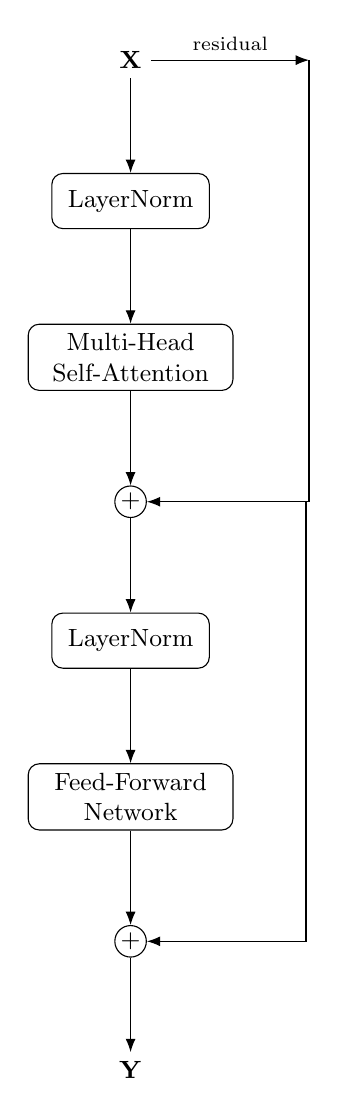
\begin{tikzpicture}[>=Latex, node distance=12mm, font=\small]
\node (x)   {$\mX$};
\node (ln0) [norm, below=of x] {LayerNorm};
\node (msa) [block, below=of ln0] {Multi-Head\\Self-Attention};
\node (add1)[plus,  below=of msa] {\small $+$};
\node (ln1) [norm,  below=of add1] {LayerNorm};
\node (ffn) [block, below=of ln1] {Feed-Forward\\Network};
\node (add2)[plus,  below=of ffn] {\small $+$};
\node (y)   [below=of add2] {$\mY$};

% main path
\draw[->] (x) -- (ln0);
\draw[->] (ln0) -- (msa);
\draw[->] (msa) -- (add1);
\draw[->] (add1) -- (ln1);
\draw[->] (ln1) -- (ffn);
\draw[->] (ffn) -- (add2);
\draw[->] (add2) -- (y);

% residuals
\coordinate (res1start) at ($(x.east)+(20mm,0)$);
\draw[->] (x.east) -- (res1start) node[midway,above] {\scriptsize residual};
\draw[->] (res1start) |- ($(add1.east)+(20mm,0)$) -- (add1.east);

\coordinate (res2start) at ($(add1.east)+(20.2mm,0)$);
\draw[->] (res2start) |- (add2.east);
\end{tikzpicture}

\small Pre-LayerNorm Transformer block
\end{minipage}%
\hfill
% ---------------- Post-LN ----------------
\begin{minipage}{0.45\textwidth}
\centering
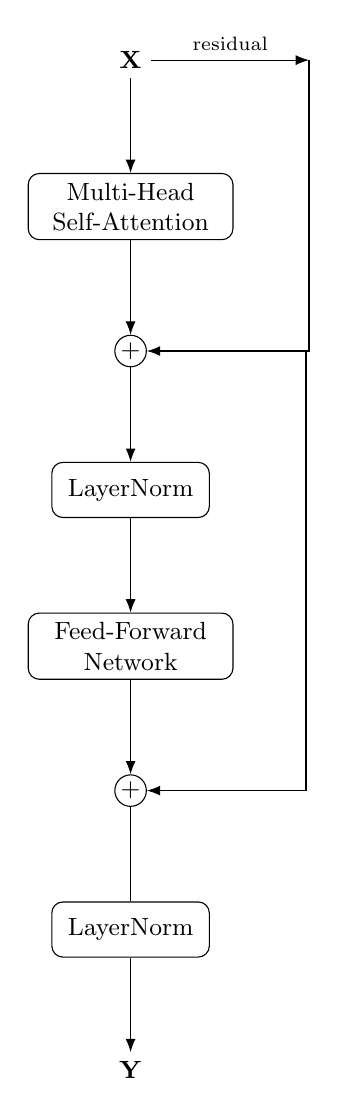
\begin{tikzpicture}[>=Latex, node distance=12mm, font=\small]
\node (x)   {$\mX$};
\node (msa) [block, below=of x] {Multi-Head\\Self-Attention};
\node (add1)[plus,  below=of msa] {\small $+$};
\node (ln1) [norm,  below=of add1] {LayerNorm};
\node (ffn) [block, below=of ln1] {Feed-Forward\\Network};
\node (add2)[plus,  below=of ffn] {\small $+$};
\node (ln2) [norm,  below=of add2] {LayerNorm};
\node (y)   [below=of ln2] {$\mY$};

% main path
\draw[->] (x) -- (msa);
\draw[->] (msa) -- (add1);
\draw[->] (add1) -- (ln1);
\draw[->] (ln1) -- (ffn);
\draw[->] (ffn) -- (add2);
\draw[->] (add2) -- (ln2) -- (y);

% residuals
\coordinate (res1start) at ($(x.east)+(20mm,0)$);
\draw[->] (x.east) -- (res1start) node[midway,above] {\scriptsize residual};
\draw[->] (res1start) |- ($(add1.east)+(20mm,0)$) -- (add1.east);

\coordinate (res2start) at ($(add1.east)+(20.2mm,0)$);
\draw[->] (res2start) |- (add2.east);
\end{tikzpicture}

\small Post-LayerNorm Transformer block
\end{minipage}

\end{figure}
As we have discussed before, the Pre-LayerNorm fashion is the current state of the art as its training is more stable, as well as its convergence. 
It helps gradient flow, and deep model stability, does not requries learning rate warm up and works better with long context.
It do has downside though, Pre-LN has a weaker normalizing effect so sometimes people add an extra final LayerNorm after the last layer for output stability (``final LN'' in GPT models).

\paragraph{Decoder}
\tikzset{
  block/.style={draw, rounded corners, minimum width=30mm, minimum height=7mm, align=center},
  norm/.style={draw, rounded corners, minimum width=22mm, minimum height=7mm, align=center},
  plus/.style={circle, draw, inner sep=0pt, minimum size=4mm},
}


\begin{figure}[H]

\centering
\begin{tikzpicture}[>=Latex, node distance=12mm, font=\small]

% --- main vertical path (Pre-LN) ---
\node (x)   {$\mX$}; % decoder input (token embeddings or previous layer output)
\node (ln0) [norm,  below=of x]   {LayerNorm};
\node (msa) [block, below=of ln0] {Masked Multi-Head\\Self-Attention};
\node (add1)[plus,  below=of msa] {\small $+$};

\node (ln1) [norm,  below=of add1] {LayerNorm};
\node (csa) [block, below=of ln1] {Multi-Head\\Cross-Attention};
\node (add2)[plus,  below=of csa] {\small $+$};

\node (ln2) [norm,  below=of add2] {LayerNorm};
\node (ffn) [block, below=of ln2] {Feed-Forward\\Network};
\node (add3)[plus,  below=of ffn] {\small $+$};
\node (y)   [below=of add3] {$y$}; % decoder output

% --- encoder memory feeding cross-attention ---
% M: encoder hidden states, shape [T_enc x d_model]
\node (memtitle) [left=34mm of csa, align=left] {Encoder memory $\mM$\\ \footnotesize $\mM \in \mathbb{R}^{L_{\text{enc}}\times d_{\text{model}}}$};
% K,V label
\node (kvlabel) [below=1mm of memtitle, anchor=north west, align=left] {\footnotesize $\mK=\mW_{\mK} \mM,\;\;\mV=\mW_V \mM$};
\draw[->] (memtitle.east) -- (csa.west) node[midway,above] {\scriptsize $\mK,\mV$};

% --- main downward arrows ---
\draw[->] (x) -- (ln0) -- (msa) -- (add1) -- (ln1) -- (csa) -- (add2) -- (ln2) -- (ffn) -- (add3) -- (y);

% --- causal mask annotation into MSA ---

\node (masknote) [right=14mm of msa, align=left] {\scriptsize causal mask \\[-1pt] \scriptsize};
\draw[-{Latex}] (masknote.west) -- ++(-4mm,0) |- (msa.east);

% Optional: label MSA inputs as Q,K,V from LN(x)
\node (qkvmsa) [left=8mm of msa, align=right] {\scriptsize $\mQ,\mK,\mV$ \\ \scriptsize from $\mathrm{LN}(\mX)$};
\draw[-{Latex}] (qkvmsa.east) -- (msa.west);


% --- residuals aligned on a right column ---
\coordinate (rcol) at ($(x.east)+(23.3mm,0)$); % common right column for loops

% residual from x to add1 with explicit origin arrow
\draw[->] (x.east) -- (rcol) node[midway,above] {\scriptsize Residual};
\draw[->] (rcol) |- (add1.east);

% residual from after add1 to add2
\draw[->] ($(add1.east)+(24mm,0)$) |- (add2.east);

% residual from after add2 to add3
\draw[->] ($(add2.east)+(24mm,0)$) |- (add3.east);

\end{tikzpicture}

\caption{Pre-LN Transformer \textbf{Decoder} block. Each sublayer consumes a LayerNormed input. The masked self-attention applies a \emph{causal mask} (no future tokens). Cross-attention queries come from the decoder stream, while keys/values are derived from the encoder memory $\mM$ (encoder hidden states: $\mK=\mW_\mK\mM$, $\mV=\mW_\mV\mM$).}
\end{figure}

As a further explanation besides the figure: this $\mM$ is the matrix of encoder hidden states produced by the last encoder layer. It is what the decoder attends to in cross attention.
Let us image that an input $\mX \in \R^{B \times L_{\text{enc}} \times d_{\text{model}}}$ is fed into the encoder blocks. 
After embedding and positional encoding, we have 
\begin{align*}
  \mH^0 \in \R^{B \times L_{\text{enc}} \times d_{\text{model}}}.
\end{align*}
Each encoder will do 
\begin{align*}
  \mH^{k+1} = \text{Encoder}(\mH^k) \in \R^{B \times L_{\text{enc}} \times d_{\text{model}}}, \quad \forall k \in [N_{\text{enc}}],
\end{align*}
And $\mM$ is exactly $\mM = \mH^{N_{\text{enc}}}$.
As a result, for the cross attention layer: $\mK, \mV \in \R^{B \times L_{\text{enc}} \times d_{\text{model}}}$ and $\mQ \in \R^{B \times L_{\text{dec}} \times d_{\text{model}}}$, so the output of decoder block will always be $\R^{B \times L_{\text{dec}} \times d_{\text{model}}}$.

The two types of blocks are different:
\begin{itemize}
  \item Encoder: Self attention only, no masking, aiming to build a contextual representation of the entire source sequence.
  
  \item Decoder: Masked self attention, which prevents seeing future tokens so that the generation is autoregressive. 
  Cross attention, which lets each target position attend to the encoder's output $\mM$ (source context)
  The purpose overall is to generate the target sequence one step at a time, with access to both past target tokens and the entire source sequence.
\end{itemize}

What happens if we are using one type?
\begin{itemize}
  \item Encoder: leaking future target tokens during training (no causal mask), so the model wouldn't learn autoregressive generation.
  \item Decoder: useless masked self-attention in the encoder that blocks half the context for no reason, waste compute on a cross-attention sublayer when no encoder memory exists yet.
\end{itemize}

\paragraph{The original seq2seq transformer:} Things happens in two phases, 
\begin{verbatim}
Source tokens ---> [Encoder stack] ----------------> M (memory)
                                         |   
                                         v
Shifted target tokens ------> [Decoder stack] ---> Output logits
\end{verbatim}
Encoder runs once on the full source, decoder runs once (training) or incrementally (inference), always starting with shifted target embeddings as its own input stream.
The input of encoder is the source sequence $x = [x_1, x_2, ..., x_{L_{\text{enc}}}]$, after embedding we get $\mX$, while the input of the decoder is the target sequence $y$ so far, but shifted ($\hat{y}$) so that the model predicts the next token.
\begin{enumerate}
  \item We take the original gold target sequence $y = [y_1, y_2, ..., y_{L_{\text{dec}}}]$.
  \item Shift right by one and add the <BOS> special token, and obtain $\hat{y} = [\text{<BOS>}, y_1, ..., y_{L_{\text{dec}} - 1}]$, we then embed to get $\hat{\mY}$ ans use it as an input to the decoder blocks.
\end{enumerate}

\subsection{Encoder only models} 
BERT, RoBERTa, DeBERTa, ELECTRA, Sentence-BERT (SBERT). 

The architecture mostly are: \textbullet~ Stacks of encoder blocks only, \textbullet~ Full self attention, \textbullet~ Input sequence length stay fixed, \textbullet~ output contextualized embeddings for every token.

Purpose: Understand text: classification, regression, retrieval, token-level labeling (NER, POS tagging, QA span prediction). In those cases the model needs bidirectional context: token sees both left and right neighbors.

For many NLP tasks, we already have the full text and just need to analyze it, not generate it.

Advantages:
\begin{itemize}
  \item \textbf{Better context capture:} every token attends to all others.
  \item \textbf{More efficient training} for non-generative tasks (no need to autoregress).
  \item \textbf{Easier fine-tuning} for classification tasks: just take the [CLS] embedding\footnote{In BERT and similar models, we prepend a special token [CLS] (“classification”) to the start of every input sequence before feeding it to the encoder. [CLS] has its own trainable embedding vector in the model's vocabulary, just like any word. It is treated as position $0$ in the sequence and goes through all encoder layers along with the other tokens. After the final encoder layer, [CLS] has a contextualized vector $h \in \R^{d_{\text{model}}}$, which encodes information from the entire sequence (thanks to self-attention).}.
\end{itemize}

The goal of encoder-only models are to learn representations of the entire input sequence.
Great for tasks like classification, NER, QA span extraction.

\paragraph{BERT pretraining in detail}
\begin{enumerate}
  \item \textbf{Input Preparation:} 
  \begin{itemize}
    \item \textbf{Tokenization:} Sentences are tokenized into WordPiece subwords.
    Special tokens are added such as [CLS] at the start (used for sequence level classification), [SEP] at the end to separate two sentences.

    \item \textbf{Segment embeddings:} BERT was designed to handle pairs of sentences, this is to let the model know which tokens belong to which sentence, so we add a segment embedding on top of the token and positional embeddings. Sentence A tokens → segment embedding ${\bf 0}$ ((vector for ``sentence A'').). Sentence B tokens → segment embedding ${\bf 1}$ ((vector for ``sentence B'').).
    
    \item \textbf{Position embeddings:} Added to encode order of tokens.
  \end{itemize}  

  \item \textbf{Masked Language Modeling (MLM):}
  \begin{itemize}
    \item \textbf{Random masking:} We select 15\% of the input tokens for possible prediction. 
    For each selected token, 80\% of the time we replace it with [MASK], 10\% of the time we replace it with a random word and 10\% of the time we keep it unchanged.
    This trick prevents the model relies too heavily on [MASK] and improves robustness.

    \item \textbf{Forward pass:} Feed the corrupted sentence into the encoder stack. 
    For each masked position $t$, get hidden representation $\mh_t$. 
    Then we apply softmax over the vocabulary 
    \begin{align*}
      p_{\theta}(\mx_t \mid \mx_{\backslash t}) = \text{softmax} \rbrac{\mW \mh_t},
    \end{align*}
    we then do cross-entropy only on masked positions 
    \begin{align*}
      \cL_{\text{MLM}}(\theta) = - \sum_{t \in \text{Masked}}\log p_\theta (\mx_t \mid \mx_{\backslash t}),
    \end{align*}
    where $\mx_{\backslash t}$ denotes the other positions than $t$.
  \end{itemize}

  \item \textbf{Next Sentence Prediction (NSP):}
  \begin{itemize}
    \item \textbf{Sentence pair construction:} 50\% of the time, we set sentence B follows sentence A in corpus (label = isNext), and the other 50\% of the time, sentence B is randomly sampled (label = notNext), we then construct them into the following format 
    \begin{verbatim}
      [CLS] Sentence A [SEP] Sentence B [SEP]
    \end{verbatim}

    \item \textbf{Classification head:} we take the [CLS] embedding $h_{\text{CLS}}$ from the final layers, and we pass through a classification layer
    \begin{align*}
      y = \text{softmax}(\mW_{\text{NSP}}\mh_{\text{CLS}}),
    \end{align*}
    where $y$ is the predicted probability output of the model, $y \in (0, 1)$, we will use $y^\star \in \cbrac{0, 1}$ to denote the true label.

    \item \textbf{Loss:} we use the binary classification loss, 
    \begin{align*}
      \cL_{\text{NSP}}(\theta) = -y^\star \log y + (1 - y^\star) \log (1 - y), 
    \end{align*} 
    This is a classic binary cross entropy loss, which can be interpreted as follows, if the sentence is indeed in such a relation, then we maximize the log likelihood this is the case, otherwise if it is not in such a relation, then we maximize the log likelihood that this is not the case.
  \end{itemize}

  \item \textbf{Total Loss:} 
  The two objectives are combined, 
  \begin{align*}
    \cL(\theta) = \cL_{\text{MLM}}(\theta) + \cL_{\text{NSP}}(\theta),
  \end{align*}
  and we continue to optimize it.
  
  \item \textbf{Extensions:} 
  We may easily notice that BERT actually produces contextual embeddings for the entire sequence via [CLS] token or pooled output, so we can actually add a classification head to predict many kinds of relations. 
  For examples: (i) Entailment / Contradiction (NLI) → [Premise] [SEP] [Hypothesis], (ii) Semantic similarity / Paraphrase → [Sentence1] [SEP] [Sentence2] (iii) Retrieval-style relevance → [Query] [SEP] [Document] (iv) Dialogue coherence → [Previous turn] [SEP] [Candidate response]

  \item \textbf{Representations:}
  We note that using the [CLS] token, we can easily get a representation of the sequence (sentence) we are working with. 
  A natural question arises, which is how we obtain such a representation for a document.
  In practice, if we are looking at short paragraphs ($< 512$ tokens: hard cap of vanilla BERT), the [CLS] token might be the right choice. 
  For medium docs (2-3 pages), we may chunk it into 512 tokens and then using max/mean/attention pooling (learn weights to combine chunks).
  For larger docs, we may consider using a hierarchical BERT (imagine here sentences are tokens) or a long-document transformer.
\end{enumerate}




\subsection{Decoder only models}

GPT family (GPT-2, GPT-3, GPT-4, LLaMA, Mistral, Falcon, etc.); BLOOM, OPT, Pythia; Code generation models (CodeLLaMA, StarCoder)

Architecture: \textbullet~ Stack of decoder blocks only \textbullet~ Causal self-attention (mask future positions) \textbullet~ \textbf{No cross-attention} \textbullet~ Input length = current sequence length during generation.

Purpose: Generate text: language modeling, code generation; model learns 
\begin{align*}
  P(\text{next token} \mid \text{prev tokens})
\end{align*}

Advantages:
\begin{itemize}
  \item \textbf{Simpler}: do not need an encoder, since we aim to predict the next token given the past. Same architecture works for both pretraining (predict next token) and inference (sample next token)
  \item \textbf{Massive scalability}: can ingest any text corpus, no need for aligned parallel data.
  \item \textbf{Flexible prompts}: can condition on arbitrary text in-context.
\end{itemize}

The goal of decoder-only models is to autoregressively generate text, good for open-ended generation.


\subsection{Encoder-decoder models}
Often on seq2seq task, requires paired data\footnote{An example is that machine translation needs paired data: Source: "I like apples", Target: "J'aime les pommes".}. 
Take an input sequence, encode it, then decode into an output (good for seq2seq tasks like translation, summarization).



\subsection{Prefix-decoder models}
Slightly less main stream variant in the tranformer family, similar to an interpolation between decoder-only and encoder-decoder models.

\textbf{Key difference:} In prefix decoder blocks, we only have one prefix self attention layer (causal self attention layer with prefix mask), and we do not have two attentions (cross attention + self attention) pattern as in the normal decoder block.
We are essentially changing the externel information from encoder to prefix region in the mask.


Imagine now we take a sequence of length $L = m + n$
\begin{align*}
  \textbf{x} = [\underbrace{p_1, \hdots, p_m}_{\textbf{p}}, \underbrace{g_1, \hdots, g_n}_{\textbf{g}}],
\end{align*}
where $\mpp$ is the prefix tokens which are given in full before text generation starts.
This could be tokens from a source sentence (like the ``encoder output'' flattened into tokens), learnable virtual tokens (prefix tuning), encoded representations from another modality (e.g., image embeddings mapped to token space),or just a long text prompt. $\mg$ here is the generation tokens that we will generate causually one by one.

A standard decoder (decoder-only transformers) uses a strict causal mask, which is a lower triangular matrix,
\begin{align*}
  \text{Mask}[i, j] = \begin{cases}
    1 &\quad \text{ if } \quad j \leq i \\
    0 &\quad \text{ otherwise }
  \end{cases}
\end{align*}
for all $i, j \in [L]$, this says that token $i$ can only attends to positions $j \leq i$.
While for a prefix decoder, we relaxes the prefix region 
\begin{align*}
  \text{Mask}[i, j] = \begin{cases}
    1 & \quad \text{ if } \quad i \leq m \text{ and } j \leq m \qquad \text{prefix attends to all prefix} \\
    1 & \quad \text{ if } \quad i \geq m \text{ and } j \leq m \qquad \text{generation attends to all prefix} \\
    1 & \quad \text{ if } \quad i > m, m < j \leq i \qquad \text{generation attends to its own past}\\
    0 & \quad \text{ otherwise }
  \end{cases}
\end{align*}

An example is that when we want to generate a translation for a sentence $\mt$ (of tokens), we will use it as a prefix, and we know that $\mt_0$ is translated into $\ms_0$ already, in this case, our prefix would be $[\mt_0, \text{<sep>}, \ms_0, \text{<BOS>}]$ and our generation tokens would be $\mt$.
We include <BOS> in the prefix because it is a known token which is used to anchor.

We prefer prefix decoder sometimes, because 
\begin{itemize}
  \item \textbf{Fewer Parameters:} Parameter in the attention part drop roughly half.
  \item \textbf{Lower compute cost:} When prefix length is modest compared to generation length, prefix decoder can be fast overall, especially on hardware where fusing the attention into one pass matters.
  \item \textbf{Simpler architecture:} Do not need a separate encoder-decoder split
  \item \textbf{Easier caching for autoregressive generation}: In standard decoder with cross attention, we need to cache (i) decoder past key/values for masked self attention (ii) the encoder outputs for cross attention.
  In a prefix decoder, the prefix tokens are just part of the same KV-cache. 
\end{itemize}
Down sides: (1) less flexibility in terms of shared layer stack and parameters. (2) for long prefixes, attention is more expansive.


\subsection{Summary}
As a summary:
\begin{table}[H]
\label{tablex1}
\centering
\renewcommand{\arraystretch}{1.2}
\begin{tabular}{|l|p{5cm}|p{5cm}|}
\hline
\textbf{Model type} & \textbf{Pros} & \textbf{Cons} \\
\hline
\textbf{Encoder-only} & 
\textbullet~ Strong understanding with bidirectional context 

\textbullet~Great for classification, retrieval, and embedding learning
& 
\textbullet~ Not suited for generative tasks \\
\hline
\textbf{Decoder-only} &
\textbullet~ Simpler architecture 

\textbullet~ Easy to train generatively 

\textbullet~ Highly flexible for any prompt-based generation
&
\textbullet~ Lacks bidirectional context

\textbullet~ Weaker for pure understanding tasks without adaptation \\
\hline
\textbf{Encoder--decoder} &
\textbullet~ Best for sequence-to-sequence tasks (translation, summarization, speech-to-text)
&
\textbullet~ Requires paired data

\textbullet~ Heavier compute at inference (two stacks) \\
\hline
\end{tabular}
\caption{Comparison of encoder-only, decoder-only, and encoder--decoder Transformer architectures.}
\end{table}


\subsection{The Linear Layers}
FFNs (Feed Forward Networks) are a part of the encoder, decoder block, there are several design choices here.
They are also known as MLPs (Multi-Layer Perceptrons), and they are used to transform the input features into a higher-dimensional space, apply non-linear activation, and then project back to the original dimension.
For the 1-$d$ case, imagine we have a vector $x \in \R^{d_{\text{model}}}$, then the FFN does the following:
\begin{align*}
  \text{FFN}(x) = \mW_2\cdot\sigma(\mW_1 x + b_1) + b_2,
\end{align*}
where $mW_1 \in \R^{d_{\text{ffn}} \times d_{\text{model}}}$ is the matrix that projects the input to a higher dimension, $\sigma$ is a non-linear activation function (e.g., ReLU, GELU), and $\mW_2 \in \R^{d_{\text{model}} \times d_{\text{ffn}}}$ projects it back to the original dimension.
$d_{\text{ffn}}$ is often $2 ~ 4 \times$ $d_{\text{model}}$.
Now if we consider the true input $\mX \in \R^{B \times L \times d_{\text{model}}}$, then basically, for each sequence in the batch, we apply the same FFN to each token, and there will be no interactions between different tokens.

\paragraph{Why do we put FFNs in the encoder/decoder blocks?}
The FFN is used to introduce non-linearity into the model, allowing it to learn more complex representations. 
Self-attention is linear in the feature dimension for a fixed set of attention weights.
It mixes tokens but does not increase the per-token expressivity much.
To see this, consider the following attention formula:
\begin{align*}
  \text{Attn}(\mQ, \mK, \mV) = \underbrace{\text{softmax}\left(\frac{\mQ\mK^\top}{\sqrt{d_{\text{model}}}}\right)}_{\eqdef \mA}\mV,
\end{align*}
if the attention weight matrix $\mA$ is fixed, then the output is a linear combination of the input $\mV$ which is linear in $\mX$, i.e, linear in the feature dimension.

If we \textbf{remove the FFN}, the model would reduce to mostly linear mixing layers accross tokens, which leads to collapse of expressivity (model underfits complex transformations), and much worse performance.


\paragraph{Design choices for FFNs:}
There are several design choices for FFNs, which can affect the model's performance and efficiency.
\begin{itemize}
  \item Expansion ratio: $d_{\text{ffn}}/d_{\text{model}}$.
\end{itemize}
This is typically around $2 ~ 4 \times$.
In the original Transformer paper, it is $4 \times$, while in LLaMA, it is $2 \times$.
In many large models, FFNs account for $50\% - 60\%$ of total parameters.

\begin{itemize}
  \item Activation function: ReLU, GELU, SiLU, etc.
\end{itemize}
The original Transformer paper uses ReLU, but GELU is more popular in modern models (BERT, GPT-2/3).

ReLU: piecewise linear, fast, but can lead to dead neurons (zero gradients for negative inputs). 
\begin{align*}
  \text{ReLU}(x) = \max(0, x).
\end{align*}

GELU: a smoother, probabilistic activation function that approximates the Gaussian distribution.
\begin{align*}
  \text{GELU}(x) = x \cdot \Phi(x) = x \cdot \frac{1}{2}\left(1 + \text{erf}\left(\frac{x}{\sqrt{2}}\right)\right),
\end{align*}
where $\Phi(x)$ is the cumulative distribution function of the standard normal distribution, and $\text{erf}$ is the error function.
\begin{itemize}
  \item Pros: \textbf{Smooth, i.e., differentiable everywhere}\footnote{Smoothness in this context refers to infinitely differentiable functions $C^{\infty}$, not the smoothness in the optimization theory sense.}, which enables better gradient flows. It often yields better performance in transformers, understanding and generation tasks.
  \item Cons: \textbf{Computationally more expensive}, sligltly more than ReLU.
\end{itemize}

SiLU: another smooth activation function, models such as EfficientNet used it. 
\begin{align*}
  \text{SiLU}(x) = x \cdot \sigma(x),
\end{align*}
where $\sigma(x) = \frac{1}{1 + e^{-x}}$ is the sigmoid function.
It is sometimes called the Swish-1 (Swish with $\beta = 1$.)


\subsection{Gated Linear Units}
GLU (Gated Linear Unit) takes an input, splits it into two parts (value \& gate), and uses one to gate the other via an elementwise product.
Mathematically, for $\mX \in \R^{B \times L \times d_{\text{model}}}$, we first apply two independent linear projections using $\mW_g, \mW_v \in \R^{d_{\text{ffn}} \times d_{\text{model}}}$, 
\begin{align*}
  \mG = \mW_g \mX + \mB_g, \qquad \mV = \mW_v \mX + \mB_v;
\end{align*}
We then apply a nonlinear activation to the gate part, after which we do elementwise multiplication.
\begin{align*}
  \mG^\prime = \sigma(\mG), \qquad \text{GLU}(\mX) = \mV \odot \mG^\prime.
\end{align*}

Note that we are applying activation to $\mG$ (the gate) instead of $\mV$, because we are applying the non-linearity here to shape its gating behaviour.
This separation between gate and value allows us to learn specialized gating pattern, which acts like an learned feature selector.

\paragraph{SwiGLU:} we are essentially replacing the original activation function $\sigma(\cdot)$ with $\text{SiLU}(\cdot)$, which is smoother. 
This is used in LLaMA, PaLM, etc.

\paragraph{GEGLU:} we are essentially replacing the original activation with $\text{GELU}(\cdot)$ or its approximations with tanh.


\subsection{Mixture-of-Experts FFNs}
In a standard Transformer block, the FFN is a single feed-forward network (sometimes gated like SwiGLU) applied to every token. 
In MoE, instead of one FFN, we have $E$ separate FFN ``experts''. 
For each token, a router chooses a subset (often 1 or 2) of experts to run.
The outputs are combined according to the router's weights.
Its advantages include 
\begin{itemize}
  \item \textbf{Scaling parameters without scaling compute:} We can have lots of experts trained but we only invoke one of them. 
  \item \textbf{Specialization:} The model specializes experts for different types of inputs (topics, syntactic structures, etc.).
\end{itemize}

Mathematically, let $\mX \in \R^{B \times L \times d_{\text{model}}}$, $E$ be the number of experts in this case. 

The forward pass:

\begin{itemize}
  \item[(i)] Router logits:
  \begin{align*}
    \mR = \mW_r \mX + \mB_r \quad \in \RBLE,
  \end{align*}
  where $\mB_r = \mathbf{1}b_r^{\top}$ is the extended bias matrix. 
  \item[(ii)] Gating probabilities:
  \begin{align*}
    \mP = \softmax (\mR) \quad \in \RBLE.
  \end{align*}

  \item[(iii)] Top-$k$ routing: 
  Keep the best-$k$ experts per token according to the probabilities, and renormalize.
  Specifically, for each token $l$ in each batch $b$, denote $\cT_k(b, l)$ as the indices of top-$k$ experts according to $\mP[b, l, :]$, we do 
  \begin{align*}
    \tilde{\mP}[b, l, d] = \frac{\mP[b, l, d]}{\sum_{j=1}^{\cT_k(b, l)}\mP[b, l, j]},\quad \forall d \in \cT_k(b, l), \quad \lvert \cT_k(b, l) \rvert = k,
  \end{align*} 
  and sets the other coordinates to be zero, which allows us to obtain $\tilde{\mP}$.
  The renormalization here is to avoid suppressing magnitude purely because we dropped low-prob experts.

  \item[(iv)] Dispatch:
  For each expert $e$, define the packed input by selecting tokens routed to $e$ as $\mX_e$.
  Let $N_e$ be the number of tokens whose top-$k$ includes expert $e$, $\pi_e(\cdot)$ be the corresponding map of expert $e$ (from $\cbrac{1, \dots, N_e} \mapsto \cbrac{[b, l]}$) to the original indices pair $(b, l)$ and let $\eta_e(\cdot)$ be the map from $\cbrac{[b, l]}$ to the index in $[N_e]$.
  Then the input for an expert is 
  \begin{align*}
    \mX_e \in \R^{N_e \times \dmodel}, \quad \text{    where    }\quad \mX_e[j, :] = \mX[\pi_e(j), :], \qquad \forall j \in [N_e]
  \end{align*}
  with the renormalized gate weight 
  \begin{align*}
    g_e \in \R^{N_e}, \quad \text{    where    }\quad g_e[j] = \tilde{\mP}[\pi_e(j), e].
  \end{align*}

  \item[(v)] Expert maps:
  Depending on the expert type (dense FFN / Gated FFN), we create 
  \begin{align*}
    \mY_e = \text{FFN}_e(\mX_e) \quad \in \R^{N_e \times \dmodel}.
  \end{align*}

  \item[(vi)] Gate scaling and combine:
  Apply per token gate (weight) to the output 
  \begin{align*}
    \tilde{\mY}_e = \diag (g_e) \cdot \mY_e, \qquad (\text{in ML literature} \qquad g_e \odot \mY_e \text{ using broadcast.}) 
  \end{align*}
  Then the output $\mZ \in \RBLDm$ would be filled such that 
  \begin{align*}
    \mZ[b, l, :] = \sum_{e \in \cT_k(b, l)} \tilde{\mY}_e[\eta_e(b, l), :]
  \end{align*}
  before outputing.
\end{itemize}

\paragraph{Capacity constraint:} In practical implementation, we often set \textbf{capacity constraint} in its formalization, which is the limit on how many tokens each expert is allowed to process in a single forward pass.
The reason to have it is 
\begin{itemize}
  \item \textbf{Load imbalance is common:} one ``hot'' expert could get far more tokens than the average, causing GPU memory overflow for that expert, and slower steps since we need to wait for it.
  \item \textbf{Hardware needs fixed allocation:} In distributed training, each expert lives on one or more GPUs, memory buffers for expert input/output must be pre-allocated. 
  If the number of tokens per expert varies wildly, we cannot pre-allocate efficiently without wasting huge amounts of memory.
\end{itemize}
We set a capacity per expert:
\begin{align*}
  C_e = \floor{\alpha \cdot \frac{BL}{E}},
\end{align*}
where $E$ is the number of experts and $\alpha \geq 1$ is the capacity factor to allow slackness. 
If an expert get more than $C_e$ tokens:
\begin{enumerate}
  \item \textbf{Dropping:} (common in Switch Transformers) Excess tokens are simply dropped for that expert: they don't get processed there, and their contribution from that expert is zeroed.
  \item \textbf{Rerouting} (less common) Excess tokens are sent to a backup expert.
\end{enumerate}
If an expert get fewer than $C_e$ tokens: one may use \textbf{padding} we pad its buffer to $C_e$ entries for vectorization but those padded entris are ignored.


\paragraph{Load balancing auxiliary loss:} 
We need an extra loss term during training so that the router doesn't collapse onto just a few experts. 
The reasion is that, without any extra incentive, the model may prefer some experts a lot more than others, leaving many experts underused or unused.
We have 
\begin{align*}
  \cL_{\text{total}} = \cL_{\text{task}} + \lambda \cdot \cL_{\text{aux}},
\end{align*}
where $\cL_{\text{task}}$ is the task loss, and in the common GShard / Switch Transfomer\footnote{Both of these are specific MoE implementations from Google that popularized large-scale sparse FFNs. Switch is basically a simplified, more efficient GShard.}, we have 
\begin{align*}
  \cL_{\text{aux}} = E \cdot \sum_{e=1}^{E} f_e \cdot m_e.
\end{align*}
$f_e$ is defined as the fraction of tokens assigned to expert $e$,
\begin{align*}
  f_e = \frac{N_e}{BL} = \frac{1}{BL}\sum_{b=1}^{B}\sum_{l=1}^{L}\mathbf{1}\cbrac{e \in \cT_k(b, l)},
\end{align*}
where $\cbrac{e \in \cT_k(b, l)}$ is the indicator vector (sum of corresponding one hot vector) in $\R^{B \times L}$ suggesting if expert $e$ is selected by this token, while $m_e$ is defined as 
\begin{align*}
  m_e = \frac{1}{BL} \sum_{b=1}^{B} \sum_{l=1}^{L} P[b, l, e],
\end{align*}
which is the average probability of assigning to expert $e$.
One can show that the loss is smaller when $f_e$ and $m_e$ are more evenly distributed across experts. 
$\cL_{\text{aux}}$ can be though of as an load balancing regularizer.

\paragraph{The all to all trick:}
In distributed training, experts are sharded across devices (e.g., $1$ expert per GPU or multiple experts per GPU.)
Naively, we must 
\begin{enumerate}
  \item Send tokens to the device hosting their assigned expert.
  \item Process them locally in the expert's feed-forward network.
  \item Send back the processed outputs to the original device to continue the model pipeline.
\end{enumerate}
This is a typical many-to-many communication patter, where  every GPU may need to send tokens to every other GPU.
The most straight forward way is to let all tokens sent to all devices before filtering using a series of all\_gather operations, but this can waste bandwitdh.

We can do it with the \textbf{all to all} trick, which use a collective communication primitive where each GPU directly sends only the tokens that the other GPUs need, in one coordinated call.
In NCCL and similar libraries
\begin{verbatim}
  torch.distributed.all_to_all_single(output, input, ...)
\end{verbatim}

In practice, MoE frameworks do two all-to-all per MoE layer:
\begin{enumerate}
  \item \textbf{Dispatch:} tokens → owning expert GPU.
  \item \textbf{Combine:} expert outputs → original token order.
\end{enumerate}
In this way, redundant communication is reduced.
Real world examples includes GShard / Switch Transformer / DeepSpeed-MoE / Megatron-MoE.

\paragraph{Processes and threads:} The legacy $\boxed{\text{nn.DataParallel}}$ (\textbf{DP}) is based on one process multi-threading, which is generally slower and less scalable (single optimizer state, host-side bottlenecks, GIL contention, extra device = host hops).
This is why \textbf{DDP} (multiprocess, one rank per GPU) is recommended.

Reasons:
\begin{enumerate}
  \item \textbf{CUDA context is per-process:} Each process gets a clean, single-GPU context, which leads to simpler, safer memory management and fewer heisenbugs.
  \item \textbf{Communication stacks (NCCL)} are designed around ranks = processes.
  \item \textbf{Python GIL:} Python threads can't execute Python bytecode truly in parallel. Many CUDA ops release the GIL(Global Interpreter Lock), but coordination/launch logic still contends. One process per GPU avoids that bottleneck.
  \item \textbf{Failure isolation:}  If one GPU OOMs or a kernel errors, you don't take down every replica in the same process.
  \item \textbf{Deterministic performance:} Independent schedulers per process avoid thread scheduling contention and reduce cross-device interference within a single interpreter.
\end{enumerate}



\subsection{Parallel Attention + FFN}
The parallel design changes the flow so that attention and FFN happen at the same time on the same input (after normalization), instead of one after the other.
Their outputs are summed together with the residual connection in a single step.
\begin{verbatim}
          ↑      → FFns      →     ↓
   x → LayerNorm → Attention → Summation
   ↓             → Residual  →     ↑
\end{verbatim}
Why do we do this:
\begin{itemize}
  \item \textbf{Parallelism:} Attention and FFN can be computed concurrently.
  \item \textbf{Fewer LayerNorms:} Saves computation.
  \item \textbf{Information Flow:} In sequential design, the FFN only sees the post-attention representation. In parallel, FFN sees the original representation directly, possibly preserving more raw token information.
  \item \textbf{Better gradient flow:} Shorter path between input and output in the computation graph.
\end{itemize}
This architecture is used in some newer LLMs, e.g. PaLM and GPT-JT, to improve speed without hurting performance.

Some practical notes:

\textbullet~ \textbf{Scaling:} Some designs scale the attention and FFN outputs to balance their contributions.
  
\textbullet~ \textbf{DropPath / Stochastic depth:} In residual networks, instead of always computing the residual branch, we may randomly drop it during training according to some probabilities, so that the model learns to rely on multiple paths, not just one.
In parallel attention, we may consider dropping attention branch and FFN branch independently. 
In this way we reduces overfitting by introducing randomness, and encourages robustness.

\textbullet~ \textbf{Variance stability:} When we sum two residual branches instead of one, we risk blowing up the variance of activations early in training. 
This is another reason why we do scaling:
\begin{align*}
  x^\prime = x + \frac{1}{\sqrt{2}}\rbrac{\text{attn\_out} + \text{ffn\_out}}
\end{align*}
We can also control by careful weight initializations, or considering set a learnable scaling parameters like $\alpha_{\text{attn}}$ and $\alpha_{\text{ffn}}$ which is small intially and train up.






\section{Computing the Number of Parameters}


\section{Fintuning}
Alignment: making the behavior of a large language model match human goals, values, or expectations.


\subsection{Pretraining Loss (self-supervised)}
As we know, in pretraining, we are basically doing a self-supervised learning task on predicting the next token.
Given an sequence $\mx = (\mx_1, \hdots, \mx_L)$, we are trying to model 
\begin{align*}
  \probsub{\theta}{\mx_1, \hdots, \mx_L} = \prod_{t=1}^L \probsub{\theta}{\mx_t \mid \mx_{< t}},
\end{align*}
where $\theta$ represnets all the trainable parameters of the language model. 
The standard choice for it is the causal language modeling (CLM) loss:
\begin{align}
  \label{eq:CLM}
  \cL_{\text{pretrain}} \rbrac{\theta} = -\frac{1}{L}\sum_{t=1}^{L}\log\rbrac{\probsub{\theta}{\mx_t \mid \mx_{<t}}}, \tag{CLM}
\end{align}
which is the negative log-likelihood over the sequence.
This can be written equivalently as the cross entropy between the model's predicted distribution $\probsub{\theta}{\cdot \mid x_{< t}} \in \R^{\lvert\cV \rvert}$ and the one-hot true token $\my_t \in \cbrac{0, 1}^{\lvert\cV \rvert}$, where $\cV$ is the vocabulary,
\begin{align}
  \label{eq:CrossEntropy}
  \cL_{\text{pretrain}}\rbrac{\theta} = -\frac{1}{L}\sum_{t=1}^{L}\sum_{v \in \cV} \rbrac{\mx^\prime_{t}}_v \log \probsub{\theta}{v \mid \mx_{<T}}, \tag{Cross Entropy}
\end{align} 
where $\rbrac{\mx^\prime_t}_v = \mathbf{1}\cbrac{v = \mx_t} \in \R^{\abs{\cV}}$.
Basically, we are summing over all possible vocabularies.
The equivalence is clear once we see that, in \eqref{eq:CrossEntropy} $\mx^\prime_t$ itself is a one hot vector, and it is $1$ nowhere but when $v = \mx_t$, with everywhere else $0$.
The training itself reduces to a \textbf{maximum likelihood} problem given a trainable set of parameter $\theta$.  
A quick implementation is that 
\begin{verbatim}
  loss = F.cross_entropy(
      logits[:, :-1, :].reshape(-1,  vocab_size), # (B, L, V) -> (BL, V)
      tokens[:, 1:].reshape(-1) # (BL, V)
    )
\end{verbatim}

\subsection{Perplexity}
Perplexity is defined as the defined as the exponential of the average loss.
For each token position, we have a prediction of the true next token $\my_t$, our model outputs a probability distribution and the loss is the corresponding negative log likelihood given by 
\begin{align*}
  - \log p_{\theta}(\my_t \mid \my_{< t}).
\end{align*} 
The perplexity is defined as 
\begin{align*}
  \exp (\Exp{- \log p_{\theta}(\my_t \mid \my_{< t})}),
\end{align*}
which is the exponential of the mean loss.
The exponential transforms the original loss which is in the log space and brings it back to the original probability space.

Intuitively, imagine reading a sentence word by word.
At each step, the model has to choose from many possible next tokens. 
If perplexity $=k$, it means the model is as ``confused'' as if it had to choose uniformly among $k$ equally likely options at each step.
That's why ppl is often described as the model's average uncertainty.

Some examples include, 
\begin{enumerate}
  \item \textbf{Perfect model} (always assigns probibility $1$ to the correct token): in this case loss $=0$, which leads to ppl $=1$.
  \item \textbf{Random guessing model} loss $= \log(\text{vocab size})$, ppl $= \text{vocab size}$.
\end{enumerate}
From this point it is easy to understand the lower the perplexity is, the better predictive power the model has.




\subsection{Finetuning Loss}
When adapting to downstream tasks or human preferences, loss functions differ.
Typical approaches include Supervised Fine-Tuning (SFT), Parameter-Efficient Fine-Tuning (PEFT) (such as LoRA and QLoRA), Reinforcement Learning from Human Feedback (RLHF)\footnote{Reinforcement learning with a reward model.}, DPO / IPO, continual pretraining, domain adaptation.

The reason for perform such finetuning is that without such adaptations, LLMs only predict next tokens, if we ask a question, they might continue the text in a way that doesn't look like an answer.


\subsubsection{Gradient Checkpointing}
Normally, during backpropagation, PyTorch needs to store all intermediate activations so it can compute gradients later. 
That eats a lot of GPU memory.
Gradient checkpointing is the technique that 
\begin{itemize}
  \item Instead of storing every intermediate activation, the model discards most of them during the forward pass.
  \item Later, during backward pass, it recomputes those activations on the fly.
  \item Saves GPU memory, but uses extra compute time.
\end{itemize}
This technique is useful when fine-tuning very large models on limited GPU memory, often lets you increase batch size or sequence length at the cost of some speed.


\subsubsection{Gradient Accumulation}
Sometimes, when the GPU does not fit the full effective batch in memory.
In this case, we split the large batch into $N$ micro-batches, and for each micro batch, we run (i) forward-backward and accumulate the gradient, but \textbf{do not} step (ii) scale the loss down by $\frac{1}{N}$ so that the accumulated gradient is correct.
After $N$ steps, we do optimizer.step() once, in this way, we can simulate a large batch size while staying within memory limits.



\subsection{Supervised Fine-Tuning (SFT)}
Our goal is to make the LLM output exactly match human-provided target completions given prompts.
Our loss is still cross-entropy loss, but computed \textbf{only} over the target part of the sequence.

Given a prompt $\mpp$ of length $L_{\mpp}$ and a target $\my$ of length $L_{\my}$, we compute 
\begin{align}
  \label{eq:lossSFT}
  \cL_{\text{SFT}} = -\frac{1}{L_{\my}} \sum_{t=1}^{L_{\my}} \log \rbrac{\probsub{\theta}{\my_t \mid \my_{< t}, \mpp}} = \frac{1}{L_{\my}}\sum_{t=1}^{L_{\my}}\sum_{v \in \cV}\rbrac{\my^\prime_t}_v\log\rbrac{\probsub{\theta}{v \mid \mpp, \my_{< t}}}, \tag{SFT}
\end{align}
where $\rbrac{\my^\prime_t}_v = \mathbf{1}\cbrac{v = \my_t} \in \R^{\abs{\cV}}$.
Notice that only completetion tokens are included in the sum (masking the prompt tokens in loss calculation).
In practice we will just mask in the following way.
\begin{align*}
  \underbrace{\text{<bos>  } \text{prompt\_tokens}}_{\text{Mask}} \text{ target\_tokens } \text{<eos>}. 
\end{align*}






\subsection{Instruction Tuning}
As we have said, pretrained LLMs (like GPT, LLaMA, Falcon, etc.) are trained on massive text corpora with the next-token prediction objective.
They learn a lot of knowledge and general linguistic ability, but they are not naturally aligned with human intent, if we ask for a list or code snippet, they may not format it correctly or if we ask a question, they might continue the text in a way that doesn't look like an answer.
Instruction tuning is a way to bridge the gap: we explicitly train the model to respond to natural-language commands (prompts) in the way humans expect.
Formally, instruction tuning $\iff$ SFT of a pretrained LLM on a dataset of \textbf{(instruction, response)} pairs.
The dataset is some times called an instruction set $\cD_{\text{instr}}$.
Let $\mx$ be instructions and $\my$ be a desired response, then 
\begin{align*}
  \cL^{\text{IT}} = - \sum_{(\mx, \my) \in \cD_{\text{instr}}} \log \pisub{\theta}{\my}{\mx},
\end{align*}
which is exactly the same as the standard language modelling loss used in finetuning \eqref{eq:lossSFT}.

\paragraph{Common instruction datasets} 
FLAN (Google): mixture of ~60 NLP tasks rephrased as natural language instructions; Alpaca: 52k instruction-response pairs generated from GPT-3;
OpenAssistant, Dolly, UltraChat, ShareGPT, etc.



\subsection{Continued Pretraining}
Continuted pretraining is the process of taking a large pretrained language model (LM) and further training it with the same pretraining objective (causal LM, masked LM, span corruption, etc.) but on a new corpus that represents the target domain, task data, or language.
This is an unsupervised adaptation method: no labels or preference data are needed.
The goal is to shift the model's distribution closer to the new data distribution without discarding general knowledge.

For a formal definition, let us image that we have $\theta_0$, which is the pretrained parameters from the base model, denote $P_{\text{base}}$ as the distribution of the original pretraining data, and $P_{\text{target}}$ as the distribution of the new data corpus (domain/task/language).
The continued pretraining then solves:
\begin{align*}
  \theta^\star = \argmin_{\theta} \ExpSub{\mx \sim P_{\text{target}}}{\cL\rbrac{\theta; x}}.
\end{align*}
which is identical on the original pretraining objective but with a shifted data distribution.



\subsection{Parameter-Efficient Fine-Tuning (PEFT)}  Updating all parameters of a model is costly. 
To resolve this, one way is to use the so called ``adaptors''.
Other approaches include LoRA, QLoRA.

\paragraph{Adaptors} In parameter-efficient fine-tuning (PEFT), adapters are small trainable modules inserted into a frozen pre-trained model's layers, typically after the feed-forward (FFN) or attention sublayer.
The core idea is that, 

\textbullet~ We freeze the original model weights.

\textbullet~ Insert a lightweight bottleneck layer (down-projection → non-linearity → up-projection) inside each transformer block.

\textbullet~ Train only these new parameters,

Mathematically, for an ouput $\mh \in \R^{\dmodel}$ (we temporarily skip the batch and sequence length dimension as we are doing this to each token's represenetation.)
\begin{align*}
  \text{Adapter}(\mh) = \mh + \mW_{\text{up}} \cdot \sigma\rbrac{\mW_{\text{down}}\mh}, 
\end{align*}
We often have $\mW_{\text{down}} \in \R^{d_{\text{down}} \times \dmodel}$ where $d_{\text{down}} << \dmodel$ so that the total number of trainable parameters are drastically reduced ($<5\%$ of the full model).


\paragraph{Low-Rank Adaptation of LLMs} Our goal here remains the same, we are trying to fine-tune large models with far fewer trainable parameters by only learning a low-rank update to certain weight matrices.

\textbullet~ \textbf{LoRA}

Formally, consider a weight matrix $\mW_0 \in \R^{\dout \times \din}$ in the pre-trained model, in stead of update its pretrained parameter $\mW_0$ directly, we keep it frozen, and learn: 
\begin{align*}
  \mW = \mW_0 + \Delta \mW, \qquad \Delta \mW = \frac{\alpha}{r}\mB\mA,
\end{align*}
where $\mA \in \R^{r \times \din}$, $\mB \in \R^{\dout \times r}$, $r$ is the low rank parameter, $\alpha$ is a scaling factor.

\begin{enumerate}
  \item Usually, LoRA is applied to attention projection matrices ($\mW_q$, $\mW_v$ and sometimes $\mW_k$, $\mW_o$).
  \item Rank $r$ and scaling $\alpha$ are hyperparams.
\end{enumerate}


Its advantage includes: 
\begin{enumerate}
  \item Drastic parameters savings.
  \item No added inference latency if merged into $\mW_0$ after training.
\end{enumerate}

Notice that empirically, touching $\mW_q$ and $\mW_v$ is basically enough since it recovers almost all the performance of full fine-tuning, while touching fewer parameters.
Intuitively, $\mW_q$ and $\mW_k$ affactes the matching space of attention.
Since $\mQ\mK^{\top}$ is bilinear, it often suffices to change $\mW_q$.  
$\mW_v$ controls the attented values and changing it also affects the post projection controlled by $\mW_o$.

There is a reason why do we apply a scaling factor here:
\begin{enumerate}
  \item \textbf{Training stability:} If $\mA$, $\mB$ are initialized with small random values, the magnitude of their product varies with $r$, and without scaling, high $r$ can produce much larger updates, destabilizing training. 
  \item \textbf{rank normalization} This keeps the expected variance of the update constant across different $r$ values. 
  $\alpha$ then allows manual controls (dependent on sensitivity).
\end{enumerate}
Empirically $\alpha = r$ or $\alpha = 1$.

The parameter $r$ controls the capacity of the low rank update.
Small $r$ means fewer trainable parameters and lower expressive power, works fine for minor domain shifts.
Large $r$ means more trainable parameters and expressive power, but if it is too large, then there is a risk of overfitting especially if training data is small. 
Empirically, $r = 4$ to $16$ common for LLaMA, GPT-J, BLOOM, etc.
Higher $r$ used in complex multi-task fine-tuning.
Futher improving $r$ often gives negligible benefits.

Usually, we initialize the matrix $\mA$ with normal initialization like kaiming\_uniform\_, but we initialize $\mB$ as all zeros.
The reason is that we need to prevent the activations we get from $\mA$ from collapsing and we also need to make sure that initially the LoRA adaptor contributed nothing to the pretrained language model, by initializing $\mB$ as all zero.
\begin{verbatim}
  self.lora_A = nn.Parameter(torch.zeros(r, d_in))
  self.lora_B = nn.Parameter(torch.zeros(d_out, r))
  nn.init.kaiming_uniform_(self.lora_A, a=math.sqrt(5))
  nn.init.zeros_(self.lora_B)
\end{verbatim}


\textbullet~ \textbf{QLoRA}
This actually refers to Quantized LoRA, which allows fine-tuning very large language models (e.g., 65B params) on a single GPU without running out of memory.
It combines $4$-bit quantization for the frozen base model and LoRA.

\begin{enumerate}
  \item Quantize $\mW_0$ to $4$-bit NormalFloat (NF4)\footnote{It is a $4$-bit quantization scheme that preserves more precision than plain int4 by using a learned normal distribution mapping.}, which cuts memory usage by $4$.
  \item Keep $\mW_0$ frozen in quantized form.
  \item Train LoRA modules $\mA$, $\mB$ in FP16 / bfloat16.
  \item During forward pass: \begin{itemize}
    \item Dequantize $\mW_0$ on the fly.
    \item Add $\Delta \mW$ from LoRA, and proceed as usual.
  \end{itemize}
\end{enumerate}

Note that there are double quantization effective in QLoRA, 
\begin{enumerate}
  \item \textbf{First quantization:} The original pretrained weight tensor $\mW_0$ is quantized from FP16/BF16 to $4$-bit NF4 values plus per-block scaling factors (distribution-aware mapping, so it preserves more accuracy than uniform int4).
  \begin{align*}
    \mW_0 = s \cdot \mW_0^{\text{quantized}}. 
  \end{align*}
  
  \item \textbf{Second quantization:} The scaling factors $s$ themselves are quantized into a lower-precision format (8-bit) plus a meta-scaling factor.
\end{enumerate}



\subsection{Reinforcement Learning from Human Feedback (RLHF)}
The goal is to train (finetune) a language model so its outputs align with human preferences by using reinforcement learning where the “reward” comes from human judgments.

Mathematically, let us first define the concept of the policy.
Given $\mx$ as an input sequence (prompt, context) and $\my$ of length $T$ as an output sequence (continuation, response), let $\pi_0(\my \mid \mx)$ be defined as the probability that he model generates $\my$ given $\mx$, defined token-by-token:
\begin{align*}
  \pi_0(\my \mid \mx) = \prod_{t=1}^T \pi_0(\my_t \mid \mx, \my_{<t}).
\end{align*}
We are using $\pi$ as our notation for it is standard in reinforcement learning\footnote{In RL, statues $s_t$ is current context (prompt + generated tokens so far), action $a_t$ is next token to generate, policy $\pi(a_t \mid s_t)$ gives the probability distribution. The pretrained LM is thus an autoregressive policy that maps states (text histories) to action distributions (token probabilities).}.

\paragraph{Stage 1: Supervised Finetuning} We prepare a supervised dataset $\cD_{\text{SFT}} = \cbrac{(\mx_i, \my_i^\star)}_{i=1}^N$ where $\mx_i$ is prompt tokens, $\my_i$ is gold-standard human-written completion (target tokens). 
Typically, the dataset size is $10^3 - 10^6$, in this stage we do standard SFT trying to minimize the cross-entropy loss on the target tokens, which can be equivalently formulated as 
\begin{align*}
  \theta_{\text{SFT}} = \arg\min_{\theta} \ExpSub{(\mx, \my^\star \sim \cD_{\text{SFT}})}{- \log \pi_{\theta}(\my^\star \mid \mx)},
\end{align*}
where 
\begin{align*}
  \log \pi_{\theta}(\my^\star \mid \mx) = \sum_{t=1}^{L_{\my^\star}}\log \pi_{\theta}\rbrac{\rbrac{\my^\star}_t \mid \mx,  \rbrac{\my^\star}_{<t}}.
\end{align*}
Basically\footnote{Here we use $\rbrac{\cdot}_t$ to denote the $t$-the component of the vector.}, we are only computing the cross entropy loss on the human labeled completions (target sequences) without touching the prompt.


\paragraph{Stage 2: Reward Modelling} We prepare a preference dataset $\cD_{\text{pref}} = \cbrac{(\mx_j, \my_j^+, \my_j^-)}_{j=1}^M$ where $\mx$ is the prompt, $\my_j^+$ is the preferred output and $\my_j^-$ is the less preferred output, $M$ is the total number of pairs of preference pairs ($10^4$ to $10^6$) coming from human labelers ranking multiple model completions for the same prompt.


\textbf{Padding:} We define the reward model $R_{\phi}(\mx, \my)$ whose input is the (input prompt tokens, completion), i.e. $(\mx, \my)$ and outputs a scalar reward score.
Typically, we start with a base language model architecture (often the same type as the policy, e.g., Transformer decoder), and we replace the usual LM head (which produces a distribution over next tokens) with a scalar regression head. 
Without the language modeling head, the output is a hidden state for each $(\mx, \my)$
\begin{align*}
  \mh = \rbrac{\mx, \my} \in \R^{B \times (L_{\mx} + L_{\my}) \times \dmodel}
\end{align*}
One may notice that for each pair of $\mx_i, \my_i$, the length $L_{\mx_i} + L_{\my_i}$ is not the same, so we must do padding in order to make it a batch \textbf{before} inputting them to the model.
We may pad all sequences on the left/right to ensure that they are the same length $L_{\max}$ to form a batch (not the global maximum, otherwise too wasteful)\footnote{This is called dynamic padding and is standard in Hugging Face DataCollatorWithPadding}, and record a corresponding attention mask $\mm_i \in \cbrac{0, 1}^{B \times L_{\max}}$ ($1$ for real token).
Often the paddings are treated as normal tokens and its embedding is either a learned vector or all zeros. 

\textbf{Batch Forming:} Now for notational convenience, let us define 
\begin{align*}
  \ms^+ = (\mx, \my^+) \in \N^{L_{\mx} + L_{\my^+}} \quad \text{ and } \quad \ms^- = (\mx, \my^-) \in \N^{L_{\mx} + L_{\my^-}},
\end{align*}
we padded them locally to form a batch $\mS = \cbrac{\hat{\ms}_1^+, {\ms}_1^-, \hdots {\ms}_B^+, {\ms}_B^-}$ where each element is now $L_{\max}$ long, with its attention mask $\mM \in \cbrac{0, 1}^{2B \times L_{\max}}$.
We feed them to the headless model and obtain 
\begin{align*}
  \mH \in \R^{2B \times L_{\max} \times \dmodel}.
\end{align*}

\textbf{Pooling:} We now need to do pooling to choose a single vector for the entire sequence to be used for pairwise comparison. 
We can choose 

\textbullet~ (A) Last-token pooling (most common), which chooses the representation of the last non-PAD tokens (since it contains context from all preceding tokens because of casual attention). 

\textbullet~ (B) Mean pooling over completions (ignore prompt tokens if we only want to summarize the generated output).

\textbullet~ (C) Special token pooling (Insert a <EOS> token and take its hidden state), works as [CLS] pooling in BERT.

After those steps, $\mH$ becomes $\mP \in \R^{2B \times \dmodel}$.

\textbf{Scalar Reward:} After we obtain $\mP$, we apply a reward head to it, which forms the reward 
\begin{align*}
  R_{\phi}(\mx, \my) = \mW_r \mP + \mb_r \in \R^{2B},
\end{align*}
where we get a scalar value for each sequence.

\textbf{Computing Loss:} We appear the pairwise Bradley-Terry loss: 
\begin{align*}
  \cL_{\text{BT}}(\phi) = -\frac{1}{B}\sum_{i=1}^{B}\log \sigma\rbrac{R_{\phi}\rbrac{\mx_i, \my_i^+} - R_\phi\rbrac{\mx_i, \my_i^-}},
\end{align*}
The above loss encourages $R_{\phi}\rbrac{\mx_i, \my_i^+}$ to be much larger than $R_{\phi}\rbrac{\mx_i, \my_i^-}$.

This is not the only way we can choose this loss, we can also pick hinge loss:
\begin{align*}
  \cL_{\text{Hinge}}(\phi) = \frac{1}{B}\sum_{i=1}^{B} \max\cbrac{0, m - \rbrac{R_{\phi}\rbrac{\mx_i, \my_i^+} - \R_\phi\rbrac{\mx_i, \my_i^-}}},
\end{align*}
where we tries to enforce a margin $m > 0$ and if that is satified, no gradient will be applied.
Compared to BT-loss, it is non-smooth.

Mean-squared error loss can also be used:
\begin{align*}
  \cL_{\text{MSE}}(\phi) = \frac{1}{B}\sum_{i=1}^{B}\rbrac{R_{\phi}\rbrac{\mx_i, \my_i^+} - \R_\phi\rbrac{\mx_i, \my_i^-} - t}^2,
\end{align*}
where $t$ is a target gap which assumed to be known (which is also the reason why it is used).

If we have more than $2$ candidates ranked, we can normalize the exponentiated rewards into a softmax, say we have $\my^1, \my^2, \hdots, \my^K$ 
\begin{align*}
  P_{\phi}(\my^j \mid \mx) = \frac{\exp\rbrac{R_{\phi}\rbrac{\mx, \my^j}}}{\sum_{j=1}^{K}\exp\rbrac{R_{\phi}\rbrac{\mx, \my^j}}},
\end{align*}
then minimize the cross entropy loss based on this,
\begin{align*}
  \cL (\phi) = - \sum_{i=1}^M\sum_{j=1}^{K} \text{prob\_of\_rank}_j \cdot \log \rbrac{P_{\phi}(\my^j \mid \mx)}, 
\end{align*}
where this prob\_of\_rank can be $1$ for the top choice and $0$ for others, or fractional.

Note that the starting point of $\phi$ is the pretrained headless model.
We can choose to use the version with/without SFT, most pipelines use the one with SFT.
\begin{enumerate}
  \item Pros 1: RM is specialized to the distribution of completions the RL stage will actually produce
  \item Pros 2: KL penalty in PPO is between two models (policy and reference) that are both in-domain with respect to RM's training data
  \item Cons 1: RM might overfit to the stylistic quirks of the SFT model and undergeneralize to very different policies
\end{enumerate}



\paragraph{Stage 3: RL fine-tuning using PPO (Proximal Policy Optimization) with KL regularization.} 
We have the reference policy after SFT, which we denote as $\pi_{\text{SFT}} = \pi_{\text{ref}}$ and the reward model $\R_{\phi}$.
Assume that now we have a prompt set $\cD_{\text{RL}}$ which are unlabeled instructions / prompt drawn from a prompt distribution (can be the same pool used in SFT, plus extra domains).

\textbf{RL objective:} We intialize our policy as $\pi_{\theta} = \pi_{\text{ref}}$, we want to now update $\pi_{\theta}$ so that it scores high under $R_{\phi}$ and stay close to $\pi_{\text{ref}}$ (to avoid drifting into low-quality or unsafe behavior), which can be described by the following KL-regularized objective:
\begin{align}
  \label{eq-obj-RL}
  \max_{\theta} \ExpSub{\substack{\mx \sim \cD_{\text{RL}} \\ \my \sim \pi_{\theta}(\cdot \mid \mx)}}{R_{\phi}(\mx, \,\my) - \beta \cdot {\rm D}_{\text{KL}}\rbrac{\pi_{\theta}(\cdot \mid \mx) \parallel \pi_{\text{ref}}(\cdot \mid x)}},
\end{align}
where $\beta > 0$ is the KL-coeffficient\footnote{Note that this is two nested expectation, first we can sample $\mx$ from the dataset, then because that the policy it self is stochastic, we have multiple possible $y$.}.
Notice that to compute the sequence level KL divergence as given above, we may decompose it into token level contribution.
For one sequence $\my = \rbrac{\my_1, \hdots, \my_T}$ generated from prompt $\mx$,
\begin{align*}
  \klD{\pisub{\theta}{\cdot}{\mx}}{\pisub{\text{ref}}{\cdot}{\mx}} = \ExpSub{\my \sim \pisub{\theta}{\cdot}{\mx}}{\sum_{t=1}^{T}\log \frac{\pisub{\theta}{\my_t}{\mx, \my_{<t}}}{\pisub{\text{ref}}{\my_t}{\mx, \my_{<t}}}},
\end{align*}
we can see that the token level contribution is given by 
\begin{align*}
  \text{KL}_t \rbrac{\mx, \my_{<t}, \my} = \log \frac{\pisub{\theta}{\my_t}{\mx, \my_{<t}}}{\pisub{\text{ref}}{\my_t}{\mx, \my_{<t}}}.
\end{align*}
If we think about it, this discourages the case that the probability of policy $\pisub{\theta}{\cdot}{\mx, \my_{<t}}$ generates $\my_t$ is smaller than that of policy $\pisub{\text{ref}}{\cdot}{\mx, \my_{<t}}$.
In practiccal training, rollouts (states, actions) are sampled from the old policy in the current outer iteration $\theta_{\text{old}}$, which is the reason why the advantage-weighted likelihood ratio ($o_t(\theta; \theta_k)$ defined later) appears.


\textbf{About KL divergence:}
Token level definition of KL divergence : at timestep $t$, the KL divergence between current policy $\pi_{\theta}$ and the reference $\pi_{\text{ref}}$ is 
\begin{align*}
  \klD{\pisub{\theta}{\cdot}{\mx, \my_{<t}}}{\pisub{\thetaref}{\cdot}{\mx, \my_{<t}}} = \sum_{\ma} \pisub{\theta}{\ma}{\mx, \my_{<t}} \cdot \log \rbrac{\frac{\pisub{\theta}{\ma}{\mx, \my_{<t}}}{\pisub{\thetaref}{\ma}{\mx, \my_{<t}}}},
\end{align*}
which is an expectation over all possible next tokens $\ma$.
The previously defined log ratio $\text{KL}_t \rbrac{\mx, \my_{<t}, \my}$ is an estimate of this true $\klD{\pisub{\theta}{\cdot}{\mx, \my_{<t}}}{\pisub{\thetaref}{\cdot}{\mx, \my_{<t}}}$ based on the one token $\my_t$, which is a random variable. We have 
\begin{align*}
  \ExpSub{\my_t \sim \pi_{\theta}}{\text{KL}_t \rbrac{\mx, \my_{<t}, \my}} = \klD{\pisub{\theta}{\cdot}{\mx, \my_{<t}}}{\pisub{\thetaref}{\cdot}{\mx, \my_{<t}}}.
\end{align*}

Even if we view it at a squence level, notice that 
\begin{align*}
  \sum_{t=1}^{T}\text{KL}_t \rbrac{\mx, \my_{<t}, \my} = \sum_{t=1}^{T}\log \rbrac{\frac{\pisub{\theta}{\ma}{\mx, \my_{<t}}}{\pisub{\thetaref}{\ma}{\mx, \my_{<t}}}} \overset{(a)}{=} \log\rbrac{\frac{\pisub{\theta}{\my}{\mx}}{\pisub{\thetaref}{\my}{\mx}}},
\end{align*}
where $(a)$ is due to the chain rule. 
This still is an estimate in the sense that 
\begin{align*}
  \ExpSub{\my \in \pisub{\theta}{\cdot}{\mx}}{\sum_{t=1}^{T}\text{KL}_t} = \klD{\pisub{\theta}{\cdot}{\mx}}{\pisub{\thetaref}{\cdot}{\mx}}.
\end{align*}
In practice, during rollouts we only compute the log-prob ratio for the tokens we sampled, because that gives us a Monte Carlo estimate of the KL penalty. 
We don't compute the full expectation KL (that would require summing over the whole vocab).


\paragraph{Sampling:} 
We can apply certain \textbf{sampling strategies} for turning the model's per-token probability distribution into actual token choices during rollout.

\textbullet~ \textbf{Temperature sampling:} assume the size of the vocabulary is $V$, for logits $\mz_t \in \R^{V}$ generated by the model at the current step $t$, we have the softmax probability 
\begin{align*}
  \mpp_i = \frac{\exp(\mz_i)}{\sum_{j=1}^{V}\exp(\mz_j)},
\end{align*} 
however, we can add another parameter which is the so called temperature $T > 0$ and rescales the logits before softmax 
\begin{align*}
  \mpp_i^{(T)} = \frac{\exp(\mz_i / T)}{\sum_{j=1}^{V}\exp(\mz_j / T)}.
\end{align*}
Observation:
\begin{enumerate}
  \item $T=1$: normal sampling from model's predicted distribution.
  \item $T>1$: flatter, more uniform, more randomness.
  \item $T<1$: sharper, more peaked, less randomness, more deterministic.
\end{enumerate}
In a word, is $T$ is high, we move to regions of smaller values which is more random, model may produce incoherent text (off-policy noise), and if $T$ is low, model keeps generating the same high-probability responses (no diversity).

\textbullet~ \textbf{Top-p sampling (nucleus sampling):} We 
sort tokens by probability $\mpp_i$ in descending order, and take the smallest set $\cS$ so that 
\begin{align*}
  \sum_{i \in \cS}^{\mpp_i} \mpp_i \geq \mpp_{\text{threshold}},
\end{align*}
where $\mpp_{\text{threshold}}$ (e.g. $0.9$) is the top-p parameter. 
Its effect is to keep most probable tokens, while cut off the long tailed improbable tokens.

\textbullet~ \textbf{Top-k sampling:} similar to other top-K.

\textbullet~ We may use them in combination, such as temperature in $[0.7, 1]$, top $p \in [0.9, 0.95]$. 
Note that they influence not only the KL divergence but also the reward model score and the learning signal diversity.

\paragraph{Computation:} 
Let us consider the $k$-th iteration for PPO and see what exactly we are going to do following the standard reinforcement learning road map.
We denote the policy parameters at the start of iteration as $\theta_k$ and the critic parameter as $\psi_k$.
\begin{enumerate}
  \item \textbf{Rollout}: We freeze policy $\theta_{\text{old}} = \theta_k$, and we sample a minibatch of prompts $\cbrac{\mx^{(1)}, \mx^{(2)}, \hdots, \mx^{(B)}} \sim \cD_{\text{RL}}$, for each prompt $\mx^{(j)}$ we generate a completion $\my^{(j)} = \cbrac{\my_1^{(j)}, \hdots, \my_{T_j}^{(j)}}$ with $\theta_{\text{old}}$ (with potential temperature sampling and others).
  For each token $t$ in each sequence, we form state $\ms_t^{(b)} = \rbrac{\mx^{(b)}, \my^{(b)}_{< t}}$, and we let action $\ma^{(b)}_t = \my_t^{(b)}$.
  We record the old log probability under $\pi_{\theta_{\text{old}}}$, 
  \begin{align*}
    \log \pisub{\theta_{\text{old}}}{\ma^{(b)}_t}{\ms^{(b)}_{t}},
  \end{align*}
  and the log probability under the reference policy 
  \begin{align*}
    \log \pisub{\theta_{\text{ref}}}{\ma^{(b)}_t}{\ms^{(b)}_{t}},
  \end{align*}
  we also evaluate the critic value $V_{\psi_k}(\ms^{(b)}_t)$ at roll-out time.
  
  \item \textbf{Learning Signals (Inner):} We may take a minibatch $\cM$ (token-step minibatch) of token steps $\cbrac{b, t}$ (optionally with a padding mask $m^{(b)}_t \in \cbrac{0, 1}$ if sequences have different lengths.)\ , we initialize $\theta = \theta_{k, 0} = \theta_k$ and $\psi = \psi_{k, 0} = \psi_k$ where we plan to run $E$ steps of update (via SGD).
  Since we have the current inner iteration policy as $\theta$, we can compute the log probability, 
  \begin{align*}
    \pisub{\theta}{\ma_t^{(b)}}{\ms_t^{(b)}},
  \end{align*}
  which allows us to compute token level KL to the reference 
  \begin{align*}
    \text{KL}_t^{(b)} = \log\pisub{\theta}{\ma_t^{(b)}}{\ms_t^{(b)}} - \log \pisub{\thetaref}{\ma_t^{(b)}}{\ms_t^{(b)}},
  \end{align*}
  and further the KL-shaping reward:
  \begin{align*}
    r_{t}^{\text{KL}, (b)} = -\beta \cdot \text{KL}_t^{(b)}.
  \end{align*}
  Then we get the per token reward 
  \begin{align*}
    r_t^{(b)}(\theta) \;=\; \begin{cases}
      r_{t}^{\text{KL}, (b)}(\theta), & t < T_b, \\[6pt]
      r_{t}^{\text{KL}, (b)}(\theta) + R_{\phi}\!\left(\mx^{(b)}, \my^{(b)}\right), & t = T_b.
    \end{cases}
  \end{align*}
  We further obtain the discounted return as  
  \begin{align*}
    G_t^{(b)}(\theta) = \sum_{l=0}^{T_b-t}\gamma^l r_{t+l}^{(b)}(\theta), 
  \end{align*}
  and the TD residual 
  \begin{align*}
    \delta_t^{(b)} = r_{t}^{(b)}(\theta) + \gamma(1 - \text{done}^{(b)}_t)V_{\psi}(\ms^{(b)}_{t+1}) - V_{\psi}(\ms^{(b)}_t),
  \end{align*}
  as well as the GAE through backward recursion 
  \begin{align*}
    \hat{A}^{(b)}_t (\theta) = \delta_t^{(b)}(\theta) + \gamma\lambda(1 - \text{done}^{(b)}_t)\hat{A}^{(b)}_{t+1} (\theta), \qquad \hat{A}^{(b)}_{T_b} (\theta) = 0.
  \end{align*}
  Then we construct the value target 
  \begin{align*}
    \hat{G}^{(b)}_t (\theta) = \hat{A}^{(b)}_t (\theta) + V_{\psi}(\ms^{(b)}_t).
  \end{align*}

  \item \textbf{PPO losses (Inner):} We first compute the importance ratio 
  \begin{align*}
    o^{(b)}_t = \exp\rbrac{\log \pisub{\theta}{\ma_t^{(b)}}{\ms_t^{(b)}} -  \log \pisub{\thetaold}{\ma_t^{(b)}}{\ms_t^{(b)}}},
  \end{align*}
  and we compute the actor loss
  \begin{align*}
    \cL^{\text{actor}}(\theta) = \frac{1}{|\cM|} \sum_{(b,t)\in \cM}\min\!\Big(o_t^{(b)}(\theta)\,\hat{A}_t^{(b)}(\theta),\,\operatorname{Clip}\!\big(o_t^{(b)}(\theta),\,1-\epsilon,\,1+\epsilon\big)\,\hat{A}_t^{(b)}(\theta)\Big),
  \end{align*}
  and critic loss
  \begin{align*}
    \cL^{\text{critic}}(\psi) = \frac{1}{|\mathcal{M}|} \sum_{(b,t)\in\mathcal{M}}\big( V_{\psi}(\ms_t^{(b)}) - \hat{G}_t^{(b)}(\theta) \big)^2,
  \end{align*}
  as well as entropy 
  \begin{align*}
    \cL^{\text{entropy}}(\theta) = \frac{1}{|\mathcal{M}|} \sum_{(b,t)\in\mathcal{M}} \Bigg[ - \sum_{\ma} \pi_{\theta}(\ma \mid \ms_t^{(b)}) \cdot \log \pi_{\theta}(\ma \mid \ms_t^{(b)}) \Bigg].
  \end{align*}
  To this end, we may form the PPO loss 
  \begin{align*}
    L^{\text{PPO}}(\theta, \psi) = L^{\text{actor}}(\theta) - c_v \cdot L^{\text{critic}}(\psi) + c_e \cdot L^{\text{entropy}}(\theta),
  \end{align*}
  where we can do gradient descent on $-\cL^{\text{PPO}}$.
  Note that we can also do an optional mask for padded tokens, if sequence are padded, we just multiplly each summand by a binary mask $m^{(b)}_t$ and divide by $\sum_{(b, t)\in \cM}m^{(t)}_b$ instead of $\abs \cM$ (Token-step minibatch convention does not need it.).
\end{enumerate}





\subsection{The Bigger Picture in Reinforcement Learning (PPO)}
In RL theory, the formal setting is a Markov Decision Process (MDP):
\begin{align*}
  \rbrac{\cS, \cA, P, r, \gamma},
\end{align*}
where 
\begin{enumerate}
  \item State $\cS$: all possible situations the agent could be in.
  In RLHF, a state $\ms_t = (\mx, \my_{<t})$.
  \item Action $\cA$: choices the agent can make.
  In RLHF, it stands for picking the next token from vocabulary.
  \item Transition function $P(\ms_{t+1} \mid \ms_t, \ma_t)$: how actions change the state.
  In RLHF: appending the chosen token to the sequence.
  \item Reward function $r(\ma_t, \ms_t)$: numeric feedback,in RLHF it is to construct KL penalty in most steps and plus the terminal reward at last.
  \item Discount factor $\gamma$: how much future rewards are worth compared to immediate ones. (In RLHF we set this to $1$ since episodes\footnote{An episode is one rollout: starting from a prompt, generating tokens until we hit an end condition (EOS token or max length).} are short.) 
\end{enumerate}

\paragraph{Objective:} Assuming we have a policy $\pisub{\theta}{\ma}{\ms}$, which is a probability distribution over actions, parameterized by $\theta$ (the weights of LLM).
The objective in RL is 
\begin{align*}
  \theta^\star = \arg\max_{\theta} J(\theta),
\end{align*}
where $J(\theta)$ is defined as 
\begin{align}
  \label{eq:J}
  J(\theta) \eqdef \ExpSub{\pi_\theta}{\sum_{t=0}^{T}\gamma^tr(s_t, a_t)}.
\end{align}
That is maximize expected total reward.
Note that the expectation actually means that we are sampling episodes (trajectories) using $\pi_{\theta}$ and for each trajectory, we compute the total discounted reward.
We average those totals over all possible trajectories, weighted by their probability of occurring under $\pi_\theta$.
For example, assume $\tau$ is a trajectory:
\begin{align*}
  \tau = \rbrac{\ms_0, \ma_0, \ms_1, \ma_1, \hdots, \ms_T, \ma_T},
\end{align*} 
with the probability $p_\theta(\tau)$
\begin{align*}
  p_{\theta}(\tau) = p(\ms_0)\prod_{t=0}^{T}\pi_{\theta}(\ma_t \mid \ms_t)\cdot p(\ms_{t+1} \mid \ms_t, \ma_t).
\end{align*}
we can rewrite $J(\theta)$ as 
\begin{align*}
  J(\theta) = \sum_{\tau} p_\theta(\tau)\cdot\sbrac{\sum_{t=0}^{T}\gamma^tr(s_t, a_t)}.
\end{align*}
Notice that we can of course think of using gradient ascent to solve this. 
However, if we define $R(\tau) \eqdef \sum_{t=0}^{T}\gamma^tr(s_t, a_t)$, notice that $R$ is the return (sum of rewards) by the environment, and it is only implicitly dependent on $\theta$ in terms of the randomness of the trajectory and if we fix one trajectory, the dependence on $\theta$ is gone.
We cannot backpropagate through this function properly.


\paragraph{Policy Gradient:}
The idea here is that 
\begin{align*}
  J(\theta) = \ExpSub{\my \sim \pi_{\theta}}{r(\my)} = \sum_{\my} \pi_{\theta}(\my) r(\my),
\end{align*}
itself is not differentiable because of the sampling process, but we can manipilate it mathematically by differentiate the expectation itself,
\begin{align*}
  \nabla_\theta J(\theta) = \nabla_\theta  \sum_{\my} \pi_{\theta}(\my) r(\my) = \sum_{\my} r(\my)\nabla_\theta \pi_\theta(\my).
\end{align*}
At this stage, everything is differentiable but we  cannot estimate by sampling, because it contains $\nabla_\theta \pi_\theta(\my)$, which we does not know, so we use the log-derivative trick to handle it mathematically again 
\begin{align*}
  \nabla_\theta \pi_{\theta}(\my) = \pi_{\theta}(\my) \nabla_\theta \log \pi_{\theta}(\my),
\end{align*}
which allows us to obtain 
\begin{align*}
  \nabla_\theta J(\theta) = \sum_{\my} r(\my)\pi_\theta(\my)\nabla_\theta \log \pi_{\theta}(\my),
\end{align*}
which is 
\begin{align*}
  \nabla_\theta J(\theta) = \ExpSub{\my \sim \pi_\theta}{r(\my)\nabla_\theta \log \pi_{\theta}(\my)}
\end{align*}
Now the gradient is expressed as an expectation over samples from $\pi_{\theta}$, so we can approximate it with Monte Carlo 
\begin{align*}
  J(\theta) \approx \frac{1}{N}\sum_{i} r(\my_i)\nabla_\theta \log \pi_\theta(\my_i).
\end{align*}


\paragraph{Details:}
As details, differentiate $J(\theta)$, we get 
\begin{align*}
  \nabla_{\theta} J(\theta) &= \int \nabla_\theta p_\theta(\tau) R(\tau) \quad d\tau \\
  &= \int p_\theta(\tau) \nabla_{\theta} \log p_{\theta}(\tau) \cdot R(\tau) \quad d\tau \\
  &= \ExpSub{\tau \sim p_\theta}{\nabla_\theta\log p_{\theta}(\tau)\cdot R(\tau)}.
\end{align*}
The environment dynamics $p(\ms_{t+1}\mid \ms_t, \ma_t)$ and $p(\ms_0)$ does not depend on $\theta$ which is just a const scaling on the original objective \eqref{eq:J}, we drop them and result in
\begin{align}
  \label{eq:A}
  \nabla_{\theta} J(\theta) = \ExpSub{\tau}{\sum_{t=0}^{T}\nabla_\theta \log \pisub{\theta}{\ma_t}{\ms_t} \cdot R(\tau)}. \tag{A}
\end{align}
This is called the \textbf{Reinforce}.
Now define the return starting at time $t$: $G_t$, which is 
\begin{align*}
  G_t \eqdef \sum_{k=t}^{T}\gamma^{k - t}r(\ms_k, \ma_k).
\end{align*}
It is a random variable depends on the future state after $t$, note that 
\begin{align*}
  R(\tau) = \underbrace{\sum_{k=0}^{t-1}\gamma^k r(\ms_k, \ma_k)}_{\text{past reward, const given $\ms_t$.}} + \gamma^t\underbrace{\sum_{k=t}^{T}\gamma^{k-t}r(\ms_k, \ma_k)}_{G_t}.
\end{align*}
For the $t$-th term in the summation in \eqref{eq:A} and \eqref{eq:J}, notice that the expectation is already conditioned on $\ma_t$ and $\ms_t$, if we remove the past reward, the gradient will not change since it is equivalent to remove a constant on $J(\theta)$, this allows us to obtain 
\begin{align}
  \label{eq:JG}
  \nabla_{\theta} J(\theta) = \ExpSub{\tau}{\sum_{t=0}^{T}\nabla_\theta \log \pisub{\theta}{\ma_t}{\ms_t} \cdot G_t}.
\end{align}
The vanilla Policy Gradient method is based on this and Monte Carlo, which is of high variance, no constraints on updates.
Now defining the \textbf{action-value} function $Q^{\pi}(\ms, \ma)$,
\begin{align*}
  Q^{\pi}(\ms, \ma) \eqdef \ExpSub{\pi}{G_t \mid \ms_t = \ms, \ma_t = \ma},
\end{align*}
which is the expected return if we are at $\ms$ state and take $\ma$ as action now, following policy $\pi$ thereafter.
The expectation itself is over the random future trajectory.
Using the tower property of expectation, we can further write 
\begin{align*}
  \nabla_{\theta} J(\theta) &= \ExpSub{\tau}{\sum_{t=0}^{T}\nabla_\theta \log \pisub{\theta}{\ma_t}{\ms_t} \cdot G_t}\\
  &= \sum_{t=0}^{T}\ExpSub{\ms_t, \ma_t}{\nabla_{\theta} \log\pisub{\theta}{\ma_t}{\ms_t}\cdot\Exp{G_t \mid \ms_t, \ma_t}} =  \sum_{t=0}^{T}\ExpSub{\ms_t, \ma_t}{\nabla_{\theta} \log\pisub{\theta}{\ma_t}{\ms_t}\cdot Q^{\pi_\theta}(\ms_t, \ma_t)}
\end{align*}
Now, for variance reduction, we introduce the state-value function:
\begin{align*}
  V^{\pi}(\ms) \eqdef \ExpSub{\ma \sim \pisub{}{\cdot}{\ms}}{Q^{\pi}(\ms, \ma)} = \ExpSub{\pi}{G_t \mid \ms_t = \ms},
\end{align*}
which is the expected return starting in state $\ms$ following $\pi$.
The advantage function is then 
\begin{align*}
  A^{\pi}(\ms, \ma) \eqdef Q^{\pi}(\ms, \ma) - V^{\pi}(s),
\end{align*}
which measure how much better the action $\ma$ is compare to the average action in state $\ms$.
Notice that for any baseline function $b(\ms_t)$ that depends only on the state $\ms_t$ but not on $\ma_t$, we observe that 
\begin{align*}
  \ExpSub{\ms_t, \ma_t}{\nabla_\theta \log \pisub{\theta}{\ma_t}{\ms_t} \cdot b(\ms_t)} &= \ExpSub{\ms_t}{b(\ms_t) \cdot \ExpSub{\ma_t}{\nabla_\theta \log \pisub{\theta}{\ma_t}{\ms_t}}} \\
  &= \ExpSub{\ms_t}{b(\ms_t) \cdot \sum_{\ma_t}\pisub{\theta}{\ma_t}{\ms_t}\nabla_\theta \log \pisub{\theta}{\ma_t}{\ms_t}} \\
  &\overset{\spadesuit}{=} \ExpSub{\ms_t}{b(\ms_t) \cdot \sum_{\ma_t}\nabla_\theta \pisub{\theta}{\ma_t}{\ms_t}} \\
  &= \ExpSub{\ms_t}{b(\ms_t) \cdot \nabla_\theta \sum_{\ma_t} \pisub{\theta}{\ma_t}{\ms_t}} = \ExpSub{\ms_t}{b(\ms_t) \cdot \nabla_\theta 1} = 0
\end{align*} 
where $\spadesuit$ is due to chain rule.
As, a result, we have 
\begin{align*}
  \nabla_{\theta} J(\theta) = \sum_{t=0}^{T}\ExpSub{\ms_t, \ma_t}{\nabla_{\theta}\log \pisub{\theta}{\ma_t}{\ms_t}\cdot \rbrac{Q^{\pi_\theta}(\ms_t, \ma_t) - b(\ms_t)}(\ms_t, \ma_t)}.
\end{align*} 
Now take $b(\ms_t) = V^{\pi_\theta}(\ms_t)$, we result in 
\begin{align*}
  \nabla_{\theta} J(\theta) = \sum_{t=0}^{T}\ExpSub{\ms_t, \ma_t}{\nabla_{\theta}\log \pisub{\theta}{\ma_t}{\ms_t}\cdot A^{\pi_\theta}(\ms_t, \ma_t)}.
\end{align*}
This is called the \textbf{policy gradient theorem}.
In practice, we still \textbf{cannot} compute $Q^{\pi_{\theta}}$ or $V^{\pi_\theta}$ exactly. 
So we train an auxiliary \textbf{value network} (Critic) to approximate $V^{\pi_\theta}$, and we estimate $A^{\pi_\theta}$ from the rollout data using methods like \textbf{Generalized Advantage Estimation} (GAE), which trades bias for variance reduction, which gives us an estimate $\hat{A}_t$.
To do this, we relies on three basic building blocks:
\begin{enumerate}
  \item \textbf{Monte Carlo (MC) return}: $G_t = \sum_{u=t}^{T}\gamma^{u - t}r_u$. 
  This is the unbiased estimate of the true return, which is very noisy and of high variance, especially if the horizon $T$ is long.

  \item \textbf{Critic (value function)}: $V_\psi \approx V^{\pi_\theta}(\ms_t) = \Exp{G_t \mid \ms_t}$, as $\theta$ is consistently changing, we need to train critic per iteration. 
  
  \item \textbf{TD residual}: $\delta_t \eqdef r_t + \gamma V_{\psi}(\ms_{t+1}) - V_\psi(\ms_t)$, which is the one step error signal telling us how much better/worse things turned out compared to the critic's expectation\footnote{If the critic is perfect, we have $V_{\psi}(\ms_t) = \Exp{r_t + \gamma V^{\pi_\theta}(\ms_{t+1})}$, this is known as Bellman expectation equation which tells us what a critic would satisfy.}.
  Notice that $\delta_t$ can be viewed as $1$-step estimate of the advantage function, since by definition (we get immediate reward + discounted value of next state)
  \begin{align*}
    Q^{\pi_\theta}(\ms_t, \ma_t) \simeq r_t + \gamma V_{\psi}(\ms_{t+1})
  \end{align*}
\end{enumerate}

\paragraph{From reward to policy update:}
We are solving a standard episodic RL problem.

\textbf{Step 1: Rollout with current policy.} 
Assume we are in iteration $k$, and we collect our trajectories by following $\pi_{\theta_k}$, this gives us data $\rbrac{\ms_t, \ma_t, r_t}$\footnote{During training, we sample many such $\mx$ from $\cD_{\text{RL}}$ in parallel, and collect a batch of rollouts at once.},
while we are collecting we also store the log probability of each action $\log \pi_{\theta_k}(\ma_t \mid \ms_t)$.

\textbf{Step 2: Advantage estimation.}
We would like to know whether each action was better or worse than average.

\textbf{Step 2.1: Train a critic.}
So we train a critic $V_{\psi_k}$ to approximate the function value $V^{\pi_\theta}$.
Usually, this $V_{\psi}$ can be a MLP parametrized by $\psi$.\footnote{In complex environments (e.g. Atari, robotics, LLMs), it can be a convolutional net, a transformer, or any architecture suited for the state representation.}
This result in an extra loss term based on MSE loss in the final PPO loss, which we name critic.

\textbf{Step 2.2: Temporal Difference (TD) residuals.}
We use the trained critic to compute $1$-step errors 
\begin{align*}
  \delta_t = r_t + \gamma (1 - \text{done}_t)V_{\psi}(\ms_{t+1}) - V_\psi(\ms_t) = \big(\text{obs reward} + \text{pred future value}\big) - \big(\text{pred value at } s_t\big),
\end{align*}
where $\text{done}_t$ is a termination flag, $\text{done}_t = 1$ means the episode has terminated at step $t$ either because the agent reached a terminal state or a time limit was reached; $\text{done}_t = 0$ means the episode continues.
When we reach the first termination iteration $T$, $1 - \text{done}_T = 0$, which means that $\delta_T = r_T - V_{\psi}(s_T)$\footnote{In RL, we use bootstrapping to denote estimating a return by combining the observed reward with the critic's estimate of the future, (instead of waiting until the very end of the episode to know the true return). Here $\gamma (1 - \text{done}_t)V_{\psi}(\ms_{t+1})$ is the bootstrap part.}. 
One may wonder why we are setting the done flag, the reason is precisely that we are handling batched data, so episodes have variable length. 
As a result, we need to pad them so that the batch is aligned, and the done flag lets us distinguish real continuation from padding or termination.
In this way, advantage/return computation stops at the right place, even inside a large batch.

If $\delta_t > 0$, the return is better than expected and the action was better than average, if $\delta_t < 0$, vice versa.
To understand this intuitively, we only have to remember that $V_{\pi_k}$ is the expected total discounted reward you will get if you start from state $\ms$ then following policy $\pi_{\theta_k}$.

\textbf{Step 2.3: Generalized Advantage Estimation (GAE).}
We have two choices to estimate advantage, one is the $1$-step estimation generated by TD-residual, which is very noisy because it only looks one step ahead, especially when we are in a long episode and there is a large reward at the end.
From an opposite point of view, if we use $G_t = r_t + \gamma r_{t+1} + \hdots$ and define 
\begin{align*}
  \hat{A}_t = G_t - V_{\psi_k}(\ms_t).
\end{align*} 
MC returns are unbiased but high variance. Using a learned critic baseline reduces variance but can introduce bias if the critic is imperfect. 

So we just combine them which results in GAE (instead of picking one horizon, we take a weighted average of all horizons).
Formally, 
\begin{align*}
  \hat{A}_t = \delta_t + \gamma\lambda\delta_{t+1} + \rbrac{\gamma\lambda}^2\delta_{t+2} + \hdots,
\end{align*}
where $\gamma = 0.99$ and $\lambda = 0.95$ are common.
Notice that $\gamma$ is the discounting factor and $\lambda$ controls how far we can look ahead.
To compute is efficiently, we use backward recursion,
\begin{align*}
  \hat{A}_t = \delta_t + \gamma\lambda\hat{A}_{t+1}.
\end{align*}
In practice, due to the padding used in batch, we set 
\begin{align}
  \hat{A}_t = \delta_t + \gamma\lambda(1 - \text{done}_t)\hat{A}_{t+1}, \qquad \hat{A}_T = 0
\end{align}
where we use a termination flag to control bootstrapping, $T$ is the index one past the last real step in the trajectory.
From the estimate $\hat{A}_t$, we can reconstruct 
\begin{align}
  \label{eq:GHAT}
  \hat{G}_t = \hat{A}_t + V_{\psi}(\ms_t), 
\end{align}
which we will later use in loss.

\textbf{Step 2.4: Gradient.} After running GAE, we now have per-time-step advantage estimates $\hat{A}_t$, which allows us to scale the log-probability gradient 
\begin{align}
  \label{eq:policy-grad}
  \nabla_{\theta} \log \pi_{\theta}(\ma_t \mid \ms_t) \cdot \hat{A}_t, \tag{Policy Gradient}
\end{align} 
where $\hat{A}_t$ increases the probability and vice versa.

\textbf{Step 3: Policy update with PPO.} Now we want to adjust $\pi_{\theta_k}$, so that actions with positive advantage become more likely, and those with negative advantage less likely.
If we use the naive policy gradient then the policy might change too much in one step.
It could also collapse (e.g., probability mass shifts to a single action, causing instability), so we need to regularize the update.
Notice that the naive objective after policy gradient transform and approximations can be written as 
\begin{align*}
  J^{\text{PG}}(\theta) = \ExpSub{t, \ms_t, \ma_t}{\log \pisub{\theta}{\ma_t}{\ms_t}\cdot \hat{A}_t}.
\end{align*}
Historically, we use \textbf{TRPO} (Trust Region Policy Optimization), where we do 
\begin{align*}
  \max_{\theta} \ExpSub{t, \ms_t, \ma_t}{r_t(\theta; 
  \theta_k) \hat{A}_t} \qquad \text{s.t.} \qquad \ExpSub{\substack{\ms \sim \rho_{\pi_{\theta_{k}}} \\ \ma \sim \pisub{\theta_{k}}{\cdot}{\ms}}}{\log\pisub{\theta_k}{\ma}{\ms} - \log\pisub{\theta}{\ma}{\ms}} \leq \delta,
\end{align*}
where $\rho_{\pi_{\theta_{k}}}$ denotes the (on-policy) state distribution under $\pi_{\theta_{k}}$ and 
\begin{align*}
  o_t(\theta; \theta_k) \eqdef \frac{\pisub{\theta}{\ma_t}{\ms_t}}{\pisub{\theta_{k}}{\ma_t}{\ms_t}},
\end{align*}
is the ratio.
The constraint can also be written equivalently as 
\begin{align*}
  \ExpSub{\ms \sim \rho_{\pi_{\theta_k}} }{\klD{\pisub{\theta_{k}}{\cdot}{\ms}}{\pisub{\theta}{\cdot}{\ms}}} \leq \delta.
\end{align*}
There are two layers of expectations: (1) over states $\ms$ that the old policy visits, (2) over actions $\ma$ drawn from the old policy at each state (this is built into the KL).
However, \textbf{TRPO} is too time consuming in the sense that it often requires second order optimization methods (conjugate gradient with Fisher-vector products to enforce the KL trust region).


\paragraph{Importance sampling based on old policy data.}  
In practice, at iteration $k$ we first collect trajectories using the current policy $\pi_{\theta_k}$. The most direct way to update would be to compute the gradient of the policy gradient objective at $\theta = \theta_k$, which is exactly on-policy with respect to the data. However, modern methods like PPO typically perform many minibatch gradient updates on the same rollout data. After the first update, the parameters have moved from $\theta_k$ to some $\theta_{k,t}$ (where $t$ indexes local iterations on this minibatch), while the data is still drawn from $\pi_{\theta_k}$. This creates a distribution mismatch: the true policy gradient is an expectation under the new policy $\pi_{\theta_{k,t}}$, but we only have samples from the old one. To address this, PPO introduces an importance-sampling correction using the ratio function
\[
  o_t(\theta; \theta_k) \;=\; \frac{\pi_\theta(\ma_t \mid \ms_t)}{\pi_{\theta_k}(\ma_t \mid \ms_t)}.
\]
The surrogate objective is then written as
\[
  \widehat{J}^{\text{PG}}(\theta; \theta_k) \;=\;
  \ExpSub{ \substack{t \\ \ms_t \sim \rho_{\pi_{\theta_k}} \\ \ma_t \sim \pi_{\theta_k}} }
  { o_t(\theta; \theta_k)\, \hat{A}^t }.
\]
Differentiating gives
\begin{align*}
  \nabla_\theta \widehat{J}^{\text{PG}}(\theta; \theta_k)
  &= \ExpSub{t,\ms_t,\ma_t}{ \nabla_\theta o_t(\theta; \theta_k)\, \hat{A}^t } \\
  &= \ExpSub{t,\ms_t,\ma_t}{ \frac{\pi_\theta(\ma_t \mid \ms_t)}{\pi_{\theta_k}(\ma_t \mid \ms_t)} \,
      \nabla_\theta \log \pi_\theta(\ma_t \mid \ms_t)\, \hat{A}^t } \\
  &= \ExpSub{t,\ms_t,\ma_t}{ o_t(\theta; \theta_k)\,
      \nabla_\theta \log \pi_\theta(\ma_t \mid \ms_t)\, \hat{A}^t }.
\end{align*}
Thus the final expression is exactly the \emph{importance-sampled version of the original policy gradient}, allowing us to reuse old-policy data $\pi_{\theta_k}$ while updating toward $\theta_{k+1}$.
This is easy to understand, we just first divide it by the probability it appears in the old disrtribution and then assigned the correct weight (the current probability) to it.
For a formal proof, we only need to use the change of measure trick in (\ref{eq:change-measure}).


\paragraph{Clipping.} If we maximize this directly, the policy can change too aggressively, leading to instability.
As a result, \textbf{PPO} in turn introduces a clipped surrogate,
\begin{align*}
  J^{\text{Clip}}(\theta; \theta_k) = \ExpSub{\substack{t \\ \ms_t \sim \rho_{\pi_{\theta_k}} \\ \ma_t \sim \pi_{\theta_k}}}{\min\cbrac{o_t(\theta; \theta_k) \hat{A}^t, \text{clip}\rbrac{o_t(\theta; \theta_k), 1-\varepsilon, 1+\varepsilon}\cdot\hat{A}^t}},
\end{align*}
where the clipping operator does the following:
\begin{enumerate}
  \item When $o_t \in [1 - \varepsilon, 1 + \varepsilon]$, we do nothing.
  \item When $o_t$ goes beyond, we replace $o_t$ by the nearest boundary value.
\end{enumerate}

\paragraph{Entropy bonus.}
If we only maximize rewards, the policy may collapse to a near-deterministic one (always picking the “best” action it has found so far).
To counter this, we add an entropy bonus to the objective.
\begin{align*}
  \cH_{\pisub{\theta}{\cdot}{\ms}} = -\sum_{\ma} \pisub{\theta}{\ma}{\ms} \log \pisub{\theta}{\ma}{\ms},
\end{align*}
if the policy is uniform then it is high.


\paragraph{Full PPO loss.}
The clipped surrogate is the policy gradient, but PPO also trains the critic and uses an entropy bonus.
\begin{align*}
  \cL^{\text{PPO}}(\theta, \psi; \theta_k) \eqdef -\underbrace{\Exp{\cJ^{\text{Clip}}(\theta; \theta_k)}}_{\text{actor}} + c_v \cdot \underbrace{\Exp{\rbrac{V_{\psi}(s_t) - \hat{G}_t}^2}}_{\text{critic}} - c_e \cdot \underbrace{\Exp{\cH\rbrac{\pisub{\theta}{\cdot}{\ms_t}}}}_{\text{exploration}},
\end{align*}
where 
\begin{align*}
  \Exp{\cH\rbrac{\pisub{\theta}{\cdot}{\ms_t}}} = \frac{1}{T}\sum_{t=0}^{T}\cH(\pisub{\theta}{\cdot}{\ms_t}).
\end{align*}



\paragraph{Practical hint.} 
In practice, the training process goes very similarly like local training where there is a nested loop:

In the $k$-th iteration, we do 
\begin{enumerate}
  \item \textbf{Rollout Phase}: We fix $\theta_{\text{old}} = \theta_{k}$ where $\theta_{\text{old}}$ denotes the frozen snapshot of the current policy.
  \begin{itemize}
    \item We use $\pi_{\theta_{\text{old}}}$ to interact with environment.
    \item We collect a batch of trajectories: states $\ms_t$, actions $\ma_t$ and reward $r_t$, we then compute the log probabilities $\log \pisub{\theta_{\text{old}}}{\ma_t}{\ms_t}$, and the old values $V_{\psi_k}(\ms_t)$, and the done flags.
  \end{itemize} 
  Imagine that there are $T$ steps across $N$ parallel environments, eventually, we got 
  \begin{align*}
    \cB = \cbrac{(\ms_t, \ma_t, r_t, \log \pi_{\text{old}(\ma_t \mid \ms_t)}, V_{\psi_k}(\ms_t), \text{done}_t)_i}_{t \in [T], i \in [N]}
  \end{align*}

  \item \textbf{Advantage + Target Computation:} 
  We compute learning signals: 
  \begin{align*}
    \delta_t = r_t + \gamma\rbrac{1 - \text{done}_t}V_{\psi_k}(\ms_{t+1}) - V_{\psi_k}(\ms_t),
  \end{align*}
  \begin{align*}
    \hat{A}_t = \delta_t + \gamma\lambda\rbrac{1 - \text{done}_t}\hat{A}_{t+1}, \qquad \hat{A}_{T} = 0,
  \end{align*}
  where $T$ is the index one past the last real step in the trajectory, and the value target 
  \begin{align*}
    \hat{G}_t = \hat{A}_t + V_{\psi_k}(\ms_t).
  \end{align*}

  \item \textbf{Update Actor \& Critic:} We initialize trainable parameter $\theta = \theta_{k, 0} = \theta_{\text{old}}$ and $\psi = \psi_{k, 0} = \psi_k$, we loop over minibatches $\cM$ of $\cB$ for several epochs $E$. 
  There are actually two types of minibatching, one is \textbf{episode level minibatching} and we are dividing based on episodes, but this can waste parallelism if episodes lengths vary a lot.
  Fortunately, we can also choose to use the \textbf{token-step minibatching}, constructing $\cM$ using token steps from different episodes.
  We use the later minibatching, and in this case $\abs \cM$ is just the total pairs of token-steps.
  \begin{enumerate}
    \item[(I)] Policy distribution under current $\theta$, 
    \begin{align*}
      \pisub{\theta}{\cdot}{\ms_t}, \quad \log\pisub{\theta}{\ma_t}{\ms_t}.
    \end{align*} 
    
    \item[(II)] Importance ratio,
    \begin{align*}
      o_t(\theta; \theta_{\text{old}}) = \exp\rbrac{\log \pisub{\theta}{\ma_t}{\ms_t} - \log \pisub{\theta_{\text{old}}}{\ma_t}{\ms_t}}
    \end{align*} 

    \item[(III)] Actor loss (clipped surrogate)
    \begin{align*}
      L^{\text{actor}} &= \ExpSub{t}{\min\cbrac{o_t(\theta; \theta_k) \hat{A}^t, \text{clip}\rbrac{o_t(\theta; \theta_k), 1-\varepsilon, 1+\varepsilon}\cdot\hat{A}^t}} \\
      &= \frac{1}{\abs \cM} \sum_{\rbrac{\ms_t, \ma_t} \in \cM} \min\cbrac{o_t(\theta; \theta_k) \hat{A}^t, \text{clip}\rbrac{o_t(\theta; \theta_k), 1-\varepsilon, 1+\varepsilon}\cdot\hat{A}^t}.
    \end{align*}
    Notice that we already do summation over time since $\abs \cM$ contains it. 

    \item[(IV)] Critic loss 
    \begin{align*}
      L^{\text{critic}} &= \ExpSub{t}{\rbrac{V_{\psi}(\ms_t) - \hat{G}_t}^2} \\
      &= \frac{1}{\abs \cM} \sum_{\ms_t \in \cM}\rbrac{V_{\psi}(\ms_t) - \hat{G}_t}^2.
    \end{align*}

    \item[(V)] Entropy bonus (exploration):
    \begin{align*}
      L^{\text{entropy}} &= \ExpSub{t}{-\sum_{\ma}\pi_\theta(\ma\mid\ms_t)\cdot\log\pi_\theta(\ma\mid\ms_t)} \\
      &= \frac{1}{\abs \cM} \sum_{\ms_t \in \cM}\rbrac{-\sum_{\ma}\pi_\theta(\ma\mid\ms_t)\cdot\log\pi_\theta(\ma\mid\ms_t)}.
    \end{align*}

    \item[(VI)] Total PPO objective 
    \begin{align*}
      L^{\text{PPO}} = - L^{\text{actor}} + c_v \cdot L^{\text{critic}} - c_e \cdot L^{\text{entropy}}.
    \end{align*}

    \item[(VII)] Take a gradient step, so that we obtain $\theta_{k, e + 1}, \psi_{k, e+1}$ from $\theta_{k, e}$ and $\psi_{k, e}$. 
  \end{enumerate}

  \item We let $\theta_{k+1} = \theta_{k, E}$ and $\psi_{k+1} = \psi_{k, E}$ using gradient ascent (or gradient descent to minus PPO loss), and prepare to enter the next iteration.
\end{enumerate}


\paragraph{Regarding the meaning of concepts}
\begin{itemize}
  \item Reward $r_t$: decided by the environment, independent of the policy, indicates how much can one get at moment $t$. 
  Normally, it depends on $\ma_t$ and $\ms_t$, i.e., $r_t = r_t(\ma_t, \ms_t)$.
  The policy do affect the realized policy since it decides what $\ma_t$ and $\ms_t$ could be.
  \item Return $G_t$: discounted cumulated future rewards, which is the total one to get from now on.
  \item Discounted factor $\gamma$, which is a number in $[0, 1]$ controlling how much future rewards matter. 
  $\gamma \approx 1$ means that we think in a long term fashion, and $\gamma$ close to $0$ suggests to live in the moment.
  \item Value function $V^{\pi}(\ms) = \ExpSub{\pi}{G_t \mid \ms_t = \ms}$, which is the expected return in state $\ms$ following policy $\pi$.
  \item Action-value function $Q^{\pi}(\ms, \ma) = \ExpSub{\pi}{G_t \mid \ms_t = \ms, \ma_t = \ma}$, which is the expected return starting in state $\ms$, taking action $\ma$.
  \item Advantage $A^{\pi}(\ms, \ma) = Q^{\pi}(\ms, \ma) - V^{\pi}(\ms)$, which has the meaning that is this move better than my usual move? This term is the key for variance reduction.
  \item Temporal difference $\delta_t = r_t + \gamma V(\ms_{t+1}) - V(\ms_t)$, where $V$ is the baseline prediction of cumulative reward. 
  $\delta_t$ is the prediction error. 
  The true value satisfies 
  \begin{align*}
    V^{\pi}(\ms_t) = \ExpSub{\pi}{r_t + \gamma V^{\pi}(\ms_{t+1})\mid \ms_t},
  \end{align*}
  which is the Bellman equation.
  \item Optimal policy $\pi^\star$, policy that maximizes expected return from every state.
\end{itemize}




\subsection{PPO-KL}
If we are using raw PPO as an alignment method, we are just optimizing against the reward model $R_{\phi}$, which may render the policy dropping into unsafe, verbose, or unnatural completions.
The solution to this is to add a KL-penalty that discourages moving too far from the reference policy (usually the SFT model).
Essentially, PPO-KL just adds an extra KL penalty term 
\begin{align*}
  J^{\text{PPO-KL}}(\theta) = J^{\text{PPO}}(\theta) - \beta\cdot\ExpSub{t}{\klD{\pisub{\theta}{\cdot}{\ms_t}}{\pisub{\thetaref}{\cdot}{\ms_t}}}.
\end{align*}
Here we follow the convention and use $J$ as the objective to maximize while $\cL$ is reserved for objective to minimize.


\subsection{DPO (Direct Preference Optimization)}
Instead of using PPO with a reward model, DPO directly optimizes the model's policy to match human preferences using a pairwise comparison dataset.
We no longer need to train or sample from a reward model at each step and we do not need complex RL machinery (advantage estimation, rollout, etc.).
Training reduces to a standard supervised loss on pairs of responses.

We will train (finetune) on a preference dataset $\cD_{\text{pref}} = \cbrac{(\mx_j, \my_j^+, \my_j^-)}_{j=1}^M$ where $\mx$ is the prompt, $\my_j^+$ is the preferred output and $\my_j^-$ is the less preferred output, $M$ is the total number of pairs of preference pairs (just like RLHF PPO stage 2).
The core idea is that we assume that there is an underlying reward function $r(\mx, \my)$ such that 
\begin{align}
  \mathbb{P}\rbrac{\my^{+} \succ \my^{-} \mid x} = \sigma\rbrac{r(\mx, \my^{+}) - r(\mx, \my^{-})}, \tag{Bradley-Terry} 
\end{align}
where $\sigma(z) = \frac{1}{1 + e^{-z}}$ is the sigmoid function.
DPO avoids learning an explicit reward model by connecting rewards to log-probabilities under the learned policy vs. a reference model (typically the SFT model):
\begin{align*}
  r(\mx, \my) \propto \beta\rbrac{\log \pisub{\theta}{\my}{\mx} - \log \pisub{\thetaref}{\my}{\mx}},
\end{align*}
where $\beta > 0$ is the temperature that controls the regularization strength.

If we plug in this into the Bradley-Terry model, we get 
\begin{align*}
  \mathbb{P}\rbrac{\my^{+} \succ \my^{-} \mid x} = \sigma\rbrac{\beta\rbrac{\log \frac{\pisub{\theta}{\my^+}{\mx}}{\pisub{\thetaref}{\my^+}{\mx}} - \log \frac{\pisub{\theta}{\my^-}{\mx}}{\pisub{\thetaref}{\my^-}{\mx}}}}.
\end{align*}
Thus we choose to maximize the likelyhood of observed preference, 
\begin{align*}
  J^{\text{DPO}}(\theta)
  &= \; \mathbb{E}_{(x, y^+, y^-) \sim \cD_{\text{pref}}}
     \Bigg[
        \log \sigma\!\Bigg(
         \tfrac{1}{\beta}\Big(
           \underbrace{\log \tfrac{\pi_\theta(y^+\mid x)}{\pi_{\mathrm{ref}}(y^+\mid x)}}_{\text{advantage of } y^+}
           \;-\;
           \underbrace{\log \tfrac{\pi_\theta(y^-\mid x)}{\pi_{\mathrm{ref}}(y^-\mid x)}}_{\text{advantage of } y^-}
         \Big)
       \Bigg)
     \Bigg],
\end{align*}
which is just a binary logistic regression (here we maximize this likelihood) objective over pairs.
The entire DPO algorithm can then be described as 
\begin{enumerate}
  \item We start with a supervised model both as $\pi_{\theta}$ and $\pi_{\text{ref}}$.
  \item We take a minibatch of paris $\cbrac{\mx_b, \my^+_b, \my^-_b}_{b=1}^B$, and we compute the log probabilities from $\pi_\theta$ and $\pi_{\text{ref}}$.
  \item We then compute the loss $\cL^{\text{DPO}}$ and backpropagate and update $\theta$.
\end{enumerate}
Notice that the $\pisub{\thetaref}{\cdot}{\mx}$ term is there to ensure that the model doesn't drift too far from the SFT model (similar to the KL penalty in PPO-RLHF).
Its advantages include 
\begin{enumerate}
  \item It directly aligns the policy with preference data.
  \item Simple, stable, and efficient: training is just supervised cross-entropy with a custom loss.
\end{enumerate}

\paragraph{Why do we assume $r$ follows the specific form?}
Consider the per prompt optimization with reward and KL-regularization, 
\begin{align*}
  \max_{\pi_{\theta}} \cbrac{\ExpSub{\my \sim \pisub{\theta}{\cdot}{\mx}}{r(\mx, \my)} - \beta\cdot\klD{\pisub{\theta}{\cdot}{\mx}}{\pisub{\thetaref}{\cdot}{\mx}}}.
\end{align*}
The objective itself is strictly concave in $\pisub{\theta}{\cdot}{\mx}$ which is a probability distribution (a vector of probabilities) over all possible $\my$.
Clearly for the first term, it is linear in $\pisub{\theta}{\cdot}{y}$, while for the second term, we have 
\begin{align*}
  -\beta\cdot\sum_{\my}\pisub{\theta}{\my}{\mx}\log\frac{\pisub{\theta}{\my}{\mx}}{\pisub{\thetaref}{\my}{\mx}},
\end{align*} 
which is also strictly concave in $\pisub{\theta}{\cdot}{\mx}$ (KL-divergence itself is convex in $\pisub{\theta}{\cdot}{\mx}$).
If we write the write the Lagrangian with normalization muiltipler $\lambda(\mx)$:
\begin{align*}
  \cL(\pi_\theta, \lambda) = \sum_{\my}\pisub{\theta}{\my}{\mx}\cdot r(\mx, \my)  - \beta \sum_{\my}\pisub{\theta}{\my}{\mx}\cdot\log \frac{\pisub{\theta}{\my}{\mx}}{\pisub{\thetaref}{\my}{\mx}} + \lambda(\mx) \rbrac{\sum_{\my}\pisub{\theta}{\my}{\mx} - 1},
\end{align*}
whose optimal condition implies 
\begin{align*}
  r(\mx, \my) - \beta\rbrac{\log \pisub{\theta}{\my}{\mx} - \pisub{\thetaref}{\my}{\mx} + 1} + \lambda(\mx) = 0.
\end{align*}
Rearrange we obtain: 
\begin{align*}
  r(\mx, \my) = \beta\rbrac{\log\pi^\star(\my\mid\mx) - \log\pisub{\thetaref}{\my}{\mx}} + C(\mx).
\end{align*}
where $C(\mx) = \lambda(\mx) + \beta$.
Since in the pariwise preference model the bias $C(\mx)$ cancels out, this justifies our choice. 
In a word, the DPO choice of $r$ comes from the PPO + KL setup, but with simplifications such as implicit reward model and sequence level loss instead of per token.


\subsection{GPRO (Generalized Preference Optimization)}
GPRO generalizes DPO further, in the sense that it instead of relying only on binary preferences (preferred vs dispreferred), it allows training with arbitrary reward functions (scalar signals, multiple preferences, or mixtures).

Consider the dataset $\cD_{\text{pref}} = \cbrac{(\mx_j, \my_j, r(\mx_j, \my_j))}_{j=1}^M$ (Different $x_j$ could be the same.).
We now define the log-ratio between policy and preference 
\begin{align*}
  z_\theta(\mx, \my) = \log \frac{\pisub{\theta}{\my}{\mx}}{\pisub{\thetaref}{\my}{\mx}}.
\end{align*}
The GPRO loss is given by 
\begin{align*}
  J^{\text{GPRO}}(\theta) = \ExpSub{\rbrac{\mx, \my} \sim \cD_{\text{pref}}}{\Omega^\star\rbrac{\beta z_\theta(\mx, \my)} - \beta r(\mx, \my)z_{\theta}(\mx, \my)},
\end{align*}
where $\Omega^\star$ is the convex conjugate of a link function $\Omega$,$\beta > 0$.
The training follows maximizing this dual objective.
In practice we use an equivalent form:
\begin{align*}
  \widehat{L}(\theta) = \sum_{x \in \cD_{\text{pref}}} \cL_{\mx}(\theta) = -\beta \sum_{\mx} \sum_{i=1}^{K_{\mx}} \omega_i(\mx)\log \pisub{\theta}{\my_i}{\mx}, \qquad \omega_i(\mx) = \frac{e^{\nicefrac{r_i(\my_i, \mx)}{\beta}}}{\sum_{j=1}^{K_{\mx}}e^{\nicefrac{r_i(\my_j, \mx)}{\beta}}}
\end{align*}


\paragraph{The intuition:} 
Fix a prompt $\mx$, consider the standard KL-regularized objective 
\begin{align*}
  \max_{\pi} \cbrac{\ExpSub{\my \sim \pisub{}{\cdot}{\mx}}{r(\mx, \my)} - \beta\cdot\klD{\pisub{}{\cdot}{\mx}}{\pisub{\thetaref}{\cdot}{\mx}}}.
\end{align*}
We will reparameterize the policy via a density ratio.
Let
\begin{align*}
  z(\my) = \log \frac{\pisub{}{\my}{\mx}}{\pisub{\thetaref}{\my}{\mx}}, \qquad u(\my) = \exp\rbrac{z(\my)} = \frac{\pisub{}{\my}{\mx}}{\pisub{\thetaref}{\my}{\mx}}.
\end{align*}
Then $\pisub{}{\my}{\mx} = \pisub{\thetaref}{\my}{\mx}u(\my)$ must normalize, i.e., 
\begin{align*}
  \sum_{\my}\pisub{\thetaref}{\my}{\mx}u(\my) = 1  \Leftrightarrow  \ExpSub{\my \sim \pisub{\thetaref}{\cdot}{\mx}}{u(\my)} = 1. 
\end{align*}
Moreover,
\begin{align*}
  \klD{\pisub{}{\cdot}{\mx}}{\pisub{\thetaref}{\cdot}{\mx}} = \ExpSub{\my \sim \pisub{}{\cdot}{\mx}}{z(\my)} 
\end{align*}
and
\begin{align}
  \label{eq:change-measure}
  \ExpSub{\my \sim \pisub{}{\cdot}{\mx}}{f(\my)} = \sum_{\my} \pisub{\thetaref}{\my}{\mx}u(\my)f(\my) =\ExpSub{\my \sim \pisub{\thetaref}{\cdot}{\mx}}{u(\my) f(\my)}.
\end{align}
As a result, taking $f(\my) = r(\mx, \my)$, we can reform the original objective as 
\begin{align*}
  \max_{u \geq 0, \ExpSub{\pisub{\thetaref}{\cdot}{\mx}}{u(\my)}=1} \cbrac{\ExpSub{\my \sim \pisub{\thetaref}{\cdot}{\mx}}{u(\my)r(\mx, \my)} - \beta\ExpSub{\my \sim \pisub{\thetaref}{\cdot}{\mx}}{u(\my)z(\my)}}, \qquad z(\my) = \log u(\my).
\end{align*}
The same conclusion also holds in the continuous case.
We form the Lagrangian for the fixed $\mx$,
\begin{align*}
  \cL\rbrac{u, \lambda} &= \ExpSub{\my \sim \pisub{\thetaref}{\cdot}{\mx}}{ur} - \beta  \ExpSub{\my \sim \pisub{\thetaref}{\cdot}{\mx}}{uz} - \lambda\rbrac{ \ExpSub{\my \sim \pisub{\thetaref}{\cdot}{\mx}}{u} - 1} \\
  &=  \ExpSub{\my \sim \pisub{\thetaref}{\cdot}{\mx}}{-\rbrac{\beta uz - ur + \lambda u} } + \lambda.
\end{align*}
Differentiate pointwisely w.r.t. $u$, we get 
\begin{align*}
  r - \beta(\log u + 1) - \lambda = 0,
\end{align*}
which suggests 
\begin{align*}
  \log u(\my) = \frac{r(\mx, \my) - \lambda - \beta}{\beta} \Rightarrow u^\star(\my) = C\cdot \exp\rbrac{\frac{r(\mx, \my)}{\beta}}, \quad \text{where} \quad C \eqdef \exp\rbrac{-\frac{\lambda + \beta}{\beta}}.
\end{align*}
Enforcing the constraint $\ExpSub{\my \sim \pisub{\thetaref}{\cdot}{\mx}}{u} = 1$, we get 
\begin{align*}
  C\cdot\ExpSub{\my \sim \pisub{\thetaref}{\cdot}{\mx}}{\exp\rbrac{\frac{r}{\beta}}} = 1 \Rightarrow C = \frac{1}{\ExpSub{\my \sim \pisub{\thetaref}{\cdot}{\mx}}{\exp\rbrac{\frac{r}{\beta}}}}.
\end{align*}
Therefore 
\begin{align*}
  u^\star(\my) = \frac{\exp\rbrac{\frac{r(\mx, \my)}{\beta}}}{\ExpSub{\my \sim \pisub{\thetaref}{\cdot}{\mx}}{\exp\rbrac{\frac{r}{\beta}}}} \quad \text{and} \quad \pi^\star(\my \mid \mx) = \pisub{\thetaref}{\my}{\mx}u^\star(y) = \frac{\pisub{\thetaref}{\my}{\mx}\exp\rbrac{\frac{r(\mx, \my)}{\beta}}}{\ExpSub{\my \sim \pisub{\thetaref}{\cdot}{\mx}}{\exp\rbrac{\frac{r(\mx,\my)}{\beta}}}}.
\end{align*}
The optimal policy is obtained by reweighting the reference distribution, so that outcomes with higher reward get exponentially more weight, this reweighting is what people called \textbf{exponential tilt}.
The optimal log ratio is given by 
\begin{align*}
  z^\star(\my) = \frac{r(\mx, \my)}{\beta} - \log \ExpSub{\my \sim \pisub{\thetaref}{\cdot}{\mx}}{\exp\rbrac{\frac{r(\mx, \my)}{\beta}}}.
\end{align*}
Since the elementwise objective is strictly concave for $u > 0$ and the constraint is affine, KKT conditions apply; complementary slackness gives an interior solution $u^\star(\my) > 0$, which makes the stationary point above a unique maximizer.
Plug it back into the primal gives the optimal value 
\begin{align*}
  \beta \log \ExpSub{\my \sim \pisub{\thetaref}{\cdot}{\mx}}{\exp\rbrac{\frac{r}{\beta}}},
\end{align*}
which is of the classic Donsker-Varadhan form, consistent with the exponential-tilt solution.
In principle, if we have explicit $r(\mx, \my)$ for all candidate responses $\my$ we could just set our policy equal to $\pi^\star$, but in practice, the reward is only given on the dataset, and even if the value is available, we need to compute 
\begin{align*}
  \ExpSub{\my \sim \pisub{\thetaref}{\cdot}{\mx}}{\exp\rbrac{\frac{r}{\beta}}},
\end{align*}
which is log-sum-exp (log-partition function) all possible completions $\my$, which is not computable.

\paragraph{The insight of GPRO:}
Instead of trying to match $\pi_{\theta}$ to the global closed form $\pi^\star$, we can design a tractable convex surrogate that drives the model's log-ratio\footnote{The question is simply: how do we train a parameterized $\pi_\theta$ so that its log-ratio $z_{\theta}$ behaves like $z_\star$ without that partition function.} 
\begin{align*}
  z_{\theta}(\my) = \log \rbrac{\frac{\pisub{\theta}{\my}{\mx}}{\pisub{\thetaref}{\my}{\mx}}},
\end{align*}
to behave as if it were the solution of that optimization.
Now introducing the convex function (entropy link) 
\begin{align*}
  \Omega(u) = \beta\rbrac{u \log u - u + 1}, \qquad \text{for} \qquad u > 0,
\end{align*}
whose convex conjugate is 
\begin{align*}
  \Omega^\star(t) = \sup_{u \geq 0}\cbrac{ut - \Omega(u)} = \beta \rbrac{e^{t/\beta} - 1}.
\end{align*}
Now we use the Fenchel-Young inequality, 
\begin{align*}
  ut - \Omega(u) \leq \Omega^\star(t)
\end{align*}
with equality achieved if and only if $u = e^{\frac{t}{\beta}}$, which means that for any $\my$, we have 
\begin{align*}
  u^\star(\my)\cdot\beta z_{\theta}(\my) - \Omega(u^\star(\my)) \leq \Omega^\star(\beta z_{\theta}(\my))
\end{align*}
Taking expectation under $\pisub{\thetaref}{\cdot}{\mx}$, we have 
\begin{align}
  \label{eq:org-1}
  \ExpSub{\my \sim \pisub{\thetaref}{\cdot}{\mx}}{u^\star(\my)\cdot\beta z_{\theta}(\my)} - \ExpSub{\my \sim \pisub{\thetaref}{\cdot}{\mx}}{\Omega(u^\star(\my))} \leq \ExpSub{\my \sim \pisub{\thetaref}{\cdot}{\mx}}{\Omega^\star(\beta z_{\theta}(\my))}.
\end{align}
For the first term, using the change of measure in \eqref{eq:change-measure}, we have
\begin{align*}
  \ExpSub{\my \sim \pisub{\thetaref}{\cdot}{\mx}}{u^\star(\my)\cdot\beta z_{\theta}(\my)} = \beta \cdot \ExpSub{\my \sim \pi^\star(\cdot \mid \mx)}{z_{\theta}(\my)},
\end{align*}
while for the second term, we have
\begin{align*}
  \ExpSub{\my \sim \pisub{\thetaref}{\cdot}{\mx}}{\Omega(u^\star(\my))} &= \beta \rbrac{\ExpSub{\my \sim \pisub{\thetaref}{\cdot}{\mx}}{u^\star(\my)\log u^\star(\my)} - \ExpSub{\my \sim \pisub{\thetaref}{\cdot}{\mx}}{u^\star(\my)} + 1} \\
  &= \beta\cdot\ExpSub{\pi^\star(\cdot\mid \mx)}{\log u^\star(\my)} \\
  &= \beta\cdot \ExpSub{\pi^\star(\cdot\mid \mx)}{\frac{r(\mx, \my)}{\beta} +  C} \\
  &= \beta\cdot \ExpSub{\pi^\star(\cdot\mid \mx)}{\frac{r(\mx, \my)}{\beta}} + \beta C.
\end{align*}
Plus this into the original inequality \eqref{eq:org-1}, we obtain 
\begin{align*}
  \beta \cdot \ExpSub{\my \sim \pi^\star(\cdot \mid \mx)}{z_{\theta}(\my)} - \rbrac{\beta\cdot \ExpSub{\pi^\star(\cdot\mid \mx)}{\frac{r(\mx, \my)}{\beta}} + \beta C} \leq \ExpSub{\my \sim \pisub{\thetaref}{\cdot}{\mx}}{\Omega^\star(\beta z_{\theta}(\my))},
\end{align*} 
which rearranges to 
\begin{align*}
  \beta \cdot \ExpSub{\my \sim \pi^\star(\cdot \mid \mx)}{z_{\theta}(\my)} - \ExpSub{\pi^\star(\cdot\mid \mx)}{{r(\mx, \my)}} &\leq \beta C + \ExpSub{\my \sim \pisub{\thetaref}{\cdot}{\mx}}{\Omega^\star(\beta z_{\theta}(\my))}, \\
  &= \beta\ExpSub{\my \sim \pisub{\thetaref}{\cdot}{\mx}}{e^{z_{\theta}(\my)} - 1}
\end{align*}
where the inequality is tight when $\log z_{\theta}(\my) = u^\star(\my) = \log z^\star(\my)$. 
This is essentially an convex upper bound that is tight when $z_{\theta}(\my) = z^\star(\my)$.
Notice that we are trying to optimize towards $z$, so we can write the above inequality as 
\begin{align*}
  \ExpSub{\my \sim \pisub{\thetaref}{\cdot}{\mx}}{\Omega^\star(\beta z_{\theta}(\my))} - \beta \cdot \ExpSub{\my \sim \pi^\star(\cdot \mid \mx)}{z_{\theta}(\my)} \geq \text{constant}.
\end{align*}
We can define the following objective from Fenchel-Young,
\begin{align*}
  \cS_{\mx}(z_\theta) \eqdef \ExpSub{\my \sim \pisub{\thetaref}{\cdot}{\mx}}{\Omega^\star(\beta z_{\theta}(\my))} - \beta \cdot \ExpSub{\my \sim \pi^\star(\cdot \mid \mx)}{z_{\theta}(\my)} - \text{constant},
\end{align*}
where $\cS_{\mx}(z_\theta) \geq 0$, $\cS_{\mx}(z_\theta) = 0$ if and only if $z = z^\star$ and clearly it is convex.
Notice that this surrogates resembles the original GPRO loss.
This surrogate serves as a way to drive $z_\theta$ to what we want without ever computing the log partition.
Notice that for the first term, we have 
\begin{align*}
  \ExpSub{\my \sim \pisub{\thetaref}{\cdot}{\mx}}{\Omega^\star(\beta z_{\theta}(\my))} = \beta \cdot \ExpSub{\my \sim \pisub{\thetaref}{\cdot}{\mx}}{e^{z_\theta}} - \beta,
\end{align*}
while 
\begin{align*}
  \ExpSub{\my \sim \pisub{\thetaref}{\cdot}{\mx}}{e^{z_\theta}} = \sum_{y \sim \pisub{\theta}{\cdot}{\mx}}\pisub{\thetaref}{\my}{\mx}\cdot\frac{\pisub{\theta}{\my}{\mx}}{\pisub{\thetaref}{\my}{\mx}} = 1.
\end{align*}
Thus we can further write 
\begin{align*}
  \cS_{\mx}(z_\theta) = - \beta \cdot \ExpSub{\my \sim \pi^\star(\cdot \mid \mx)}{z_{\theta}(\my)},
\end{align*}
leaving out the constant.
Differentiate it w.r.t $\theta$, and notice that 
\begin{align*}
  \nabla_\theta z_\theta(\my) = \nabla_\theta \log \pisub{\theta}{\my}{\mx}. 
\end{align*}
Hence 
\begin{align*}
  \nabla_\theta \cS_{\mx}(z_\theta) = - \beta \cdot \ExpSub{\my \sim \pi^\star(\cdot\mid \mx)}{\nabla_{\theta} \log \pisub{\theta}{\my}{\mx}},
\end{align*}
which is the population gradient we want to estimate from data.
Notice that we can not compute the term $\ExpSub{\my \sim \pi^\star(\cdot \mid \mx)}{f(\my)}$ directly because we do not know the distribution, however, we can estimate it, with rewards.
We have 
\begin{align*}
  \ExpSub{\my \sim \pi^\star(\cdot \mid \mx)}{f(\my)} &= \sum_{\my \sim \pi^\star(\cdot \mid \mx)} \pi^\star(\my \mid \mx) \cdot f(\my) \\
  &= \frac{\pisub{\thetaref}{\my}{\mx}\exp\rbrac{\frac{r(\mx, \my)}{\beta}} \cdot f(\my)}{\ExpSub{\my \sim \pisub{\thetaref}{\cdot}{\mx}}{\exp\rbrac{\frac{r(\mx,\my)}{\beta}}}} =  \frac{\ExpSub{\my \sim \pisub{\thetaref}{\cdot}{\mx}}{\exp\rbrac{\frac{r(\mx, \my)}{\beta}} \cdot f(\my)}}{\ExpSub{\my \sim \pisub{\thetaref}{\cdot}{\mx}}{\exp\rbrac{\frac{r(\mx,\my)}{\beta}}}}.
\end{align*}
Assume for prompt $\mx$, we have $K$ responses with rewards $\cbrac{\rbrac{\my_i, r_i}}_{i=1}^{K_{\mx}}$, then we can estimate the expectation using\footnote{This is the key, the expectation itself is easier to estimate than the distribution.} 
\begin{align*}
  \ExpSub{\my \sim \pi^\star(\cdot \mid \mx)}{f(\my)} \approx \frac{\frac{1}{K}\sum_{i=1}^{{K_{\mx}}}e^{\nicefrac{r_i}{\beta}} f(\my_i)}{\frac{1}{{K_{\mx}}}\sum_{i=1}^{{K_{\mx}}}e^{\nicefrac{r_i}{\beta}}} = \sum_{i=1}^{{K_{\mx}}} \omega_i(\mx) f(\my_i), \qquad \omega_i(\mx) \eqdef \frac{e^{\nicefrac{r_i}{\beta}}}{\sum_{i=1}^{{K_{\mx}}}e^{\nicefrac{r_i}{\beta}}},
\end{align*}
where the problematic 
As a result, the estimated gradient is given by 
\begin{align*}
  \nabla_\theta \cS_{\mx}(z_\theta) \approx -\beta\cdot\sum_{i=1}^{{K_{\mx}}}\omega_i(\mx) \nabla_\theta \log \pisub{\pi_\theta}{\my_i}{\mx},
\end{align*}
which is a \textbf{weighted negative log-likelihood}. corresponding to 
\begin{align*}
  \widehat{\cL}_{\mx}(\theta) \eqdef -\beta \cdot \sum_{i=1}^{{K_{\mx}}}\omega_i(\mx) \log \pisub{\theta}{\my_i}{\mx},
\end{align*}
if we further aggregate over prompts 
\begin{align*}
  \widehat{L}(\theta) =  \sum_{x \in \cD_{\text{pref}}} \cL_{\mx}(\theta) = -\beta \sum_{\mx} \sum_{i=1}^{K_{\mx}} \omega_i(\mx)\log \pisub{\theta}{\my_i}{\mx},
\end{align*}
which is clearly equivalent to the original GPRO dual loss, since it is our starting point (denoted as $\cS_{\mx}(z_\theta)$ here). 
Note that we are trying to minimize this loss as we are trying to minimizer $\cS_{\mx}$.

\paragraph{Relation to DPO}
DPO is related to GPRO, let a training item be a pair $(\mx, \my^+, \my^-)$ with the label $\my^+ \succ \my^-$.
From the GPRO analysis, we have 
\begin{align*}
  z^\star(\mx, \my) = \frac{r(\mx, \my)}{\beta} - \log \ExpSub{\my \sim \pisub{\thetaref}{\cdot}{\mx}}{\exp\rbrac{\frac{r(\mx, \my)}{\beta}}},
\end{align*}
the second partition term is eliminated if we take 
\begin{align*}
  \Delta z^\star(\mx, \my^+, \my^-) = z^\star(\mx, \my^+) - z^\star(\mx, \my^-) = \frac{r(\mx, \my^+) - r(\mx, \my^-)}{\beta}.
\end{align*}
If preferences follow a Bradley-Terry (logistic) model with temperature, then, we have 
\begin{align*}
  \mathbb{P}(\my^+ \succ \my^- \mid \mx) = \sigma \rbrac{\frac{r(\mx, \my^+) - r(\mx, \my^-)}{\beta}} = \sigma \rbrac{\Delta z^\star(\mx, \my^+, \my^-)}.
\end{align*}
To make $z_{\theta}$ mimics $z_\star$, we apply a pairwise logistic surrogate to the margin, 
\begin{align*}
  m_{\theta}(\mx; \my^+, \my^-) &\eqdef \frac{1}{\beta}\rbrac{z_{\theta}(\mx, \my^+) - z_{\theta}(\mx, \my^-)} \\
  &= \frac{1}{\beta}\rbrac{\log\pisub{\theta}{\my^+}{\mx} - \log\pisub{\theta}{\my^-}{\mx} - \log\pisub{\thetaref}{\my^+}{\mx} + \log\pisub{\thetaref}{\my^-}{\mx}}.
\end{align*}
The DPO loss is exactly the logistic loss that pushes $m^\theta$ to $\Delta z^\star$, i.e.,
\begin{align*}
  L^{\text{DPO}}(\theta) = -\ExpSub{(\mx,\my^+, \my^-)}{\log\sigma\rbrac{m_\theta(\mx; \my^+, \my^-)}}
\end{align*}
Note that this is something to minimize, and in the original introduction to DPO, we are writing the goal in terms of maximization.
If we differentiate with respect to $\theta$, we get 
\begin{align*}
  \nabla_{\theta}\rbrac{ - \log \sigma (m_\theta)} &= -\sigma(-m_\theta) \cdot \nabla_\theta m_\theta \\
  &= -\frac{\sigma(-m_\theta)}{\beta}\rbrac{\nabla_\theta \log\pisub{\theta}{\my^+}{\mx} - \nabla_\theta \log\pisub{\theta}{\my^-}{\mx}} \\
  &= -\frac{1}{\beta}\rbrac{\sigma(-m_\theta)\nabla_\theta \log\pisub{\theta}{\my^+}{\mx} - \sigma(-m_\theta)\nabla_\theta \log\pisub{\theta}{\my^-}{\mx}}.
\end{align*}
As we can see, this is a weighted sum of the log-likelihood gradients, but the coefficient of the less preferred sample is negative, which means that one ``weight'' is negative. 
It is not representable as a weighted Negative Log Likelihood (NLL) form, GPRO generalizes DPO in spirits.
To be specific, DPO uses a pairwise logistic surrogate focuses only on to relative differences, which leads to negative coefficients for the dispreferred sample.


\paragraph{Relation to PPO and its implementation}
Let us recall the entire PPO objective:
\begin{align*}
  J^{\text{PPO}}(\theta) &= \mathbb{E}_{\substack{(\ms_t, \ma_t) \sim \pi_{\text{old}}}}\big[\min\cbrac{o_t(\theta; \theta_k) \hat{A}^t, \text{clip}\rbrac{o_t(\theta; \theta_k), 1-\varepsilon, 1+\varepsilon}\cdot\hat{A}^t} \\
  & \quad - \beta \cdot \klD{\pisub{\theta}{\cdot}{\ms_t}}{\pisub{\thetaref}{\cdot}{\ms_t} + \lambda_{\text{ent}} H(\pisub{\theta}{\cdot}{\ms_t})}\big].
\end{align*}
There is one implicit constraint here, that is, we do clipping to ensure that the ration is in a certain range, which enforces we are not deviating too much from the old policy $\thetaold$, this increases stability.
There is also an explicit constraint via KL divergence, which prevents the policy deviating too much from the reference policy $\thetaref$.
Here the $o_t$ is defined as: 
\begin{align*}
  o_t(\theta; \theta_k) = \frac{\pi_{\theta}(\ma_t \mid \ms_t)}{\pi_{\text{old}}(\ma_t \mid \ms_t)} = \frac{\pi_{\theta}(\ma_t \mid \ms_t)}{\pi_{\theta_k}(\ma_t \mid \ms_t)}.
\end{align*}

In GPRO, we simpliy removes the arbitrary clipping term, and anchor everything to the referrence model $\pi_{\thetaref}$.
We can write the GPRO objective as:
\begin{align*}
  J^{\text{GPRO}}(\theta) &= \mathbb{E}_{\substack{(\ms_t, \ma_t) \sim \pi_{\theta_k}}}\big[o_t(\theta; \thetaref) \hat{A}^t - \beta_k \cdot \klD{\pisub{\theta}{\cdot}{\ms_t}}{\pisub{\thetaref}{\cdot}{\ms_t} + \lambda_{\text{ent}} H(\pisub{\theta}{\cdot}{\ms_t})}\big].
\end{align*}
which is the on policy version of the GPRO objective.
Here the $o_t(\theta; \thetaref)$ is defined as:
\begin{align*}
  o_t(\theta; \thetaref) = \frac{\pi_{\theta}(\ma_t \mid \ms_t)}{\pi_{\thetaref}(\ma_t \mid \ms_t)}.
\end{align*}
Notice that we will use $\beta_k$ as a dynamic controller to control the KL divergence, and it will be updated in each iteration.
If the KL exceeds the target, we will increase $\beta_k$, otherwise, we will decrease $\beta_k$.
Notice that sometimes we will see $o_t(\theta; \thetaref)$ which is called the ratio format, while sometimes we will see $\log \pi(\ma_t \mid \ms_t)$, which is the log format, and they are equivalent from the derivation of the policy gradient method.
This is the on policy GPRO, sometimes we will see the off policy version, where we use $\pi_{\thetaref} = \mu$, i.e., the behavior policy, the rollouts are generated from this behavoir policy and we need the importance sampling trick to correct the distribution mismatch.
In practice, if we use $\mu = \theta_k$ which is the current policy, then it is the same as the on policy version, we can also let it be some old policy, which allows us to reuse the rollouts generated from the old policy, or we can let it be the reference policy, which allows us to reuse the rollouts generated from the reference policy.
Note that PPO fixes $\mu = \pi_{\text{old}}$ which is the old policy.


\paragraph{Group}
In GRPO, we do not treat each response-prompt pair independently.
Instead, we group multiple responses (and their rewards) that share the same prompt into a group, so we can compare them and apply relative regularization or preference-based objectives.

\textbullet~ \textbf{Preference-based objective:} For a pair of responses $\my^{+}$ and $\my^{-}$, a preference model (human or reward model) tells us $r^+ > r^-$.
Then the preference-based loss (as in DPO or GPRO) tries to enforces
\begin{align*}
  \log \pi_\theta(\my^+ \mid \mx) - \log \pi_\theta(\my^- \mid \mx) 
\end{align*} 
should be large.
This is equivalent to minimize 
\begin{align*}
  -\log \sigma \rbrac{\beta\rbrac{\log\frac{\pi_\theta(\my^+\mid\mx)}{\pi_{\theta}(\my^- \mid\mx)} - \log\frac{\pi_{\thetaref}(\my^+\mid\mx)}{\pi_{\thetaref}(\my^- \mid\mx)}}},
\end{align*}
which is a relative formulation.


\textbullet~ \textbf{Relative regularization:} In GRPO, we extend this to groups of size $\geq$ 2 (say 4).
For each group of responses $\cbrac{\my_1, \my_2, \my_3, \my_4}$ for the same prompt $\mx$, we compute relative preferences using a reward model or normalized scores 
\begin{align*}
  \omega_i = \frac{\exp(\beta r_i)}{\sum_{j} \exp(\beta r_j)},
\end{align*}
then optimize policy probabilities to match this distribution, 
\begin{align*}
  \min_\theta \klD{\omega_i}{\frac{\pi_{\theta}(\my_i \mid \mx)}{Z_{\theta}(x)}},
\end{align*}
where $Z_{\theta}(x) = \sum_{j} \pi_\theta(\my_i \mid \mx)$.
One thing to notice is that we do not actually compute the term explicitly, as it has already been captured by the advantage estimate.

\paragraph{Practical Hint:}
In practice, for each prompt $\mx_i$, we sample a group of $K$ resposnes, 
\begin{align*}
  \cbrac{\my_{i1}, \my_{i2}, \hdots, \my_{iK}} \sim \pi_{\theta}(\cdot \mid \mx_i),
\end{align*}
and use the corresponding reward $r_{ik}$ to compute the \textbf{group standardrized advantage}
\begin{align*}
  \hat{A}_{ik} = \frac{r_{ik} - \bar{r}_i}{\sigma_i + \varepsilon}, \qquad \text{where } \bar{r}_i = \frac{1}{K}\sum_{k=1}^{K}r_{ik}, \sigma_i = \sqrt{\frac{1}{K}\sum_{k=1}^{K} (r_{ik} - \bar{r}_i)^2}.
\end{align*} 
The GPRO loss can be written as 
\begin{align*}
  J^{\text{GRPO}} = \ExpSub{(\mx, \my) \sim \pi_{\theta}}{\hat{A}(\mx, \my)\cdot\log \pi_{\theta}(\my \mid \mx)}.
\end{align*}
Optionally, we can add a KL penalty term 
\begin{align*}
  J^{\text{GRPO-reg}} = \ExpSub{(\mx, \my) \sim \pi_{\theta}}{\hat{A}(\mx, \my)\cdot\log \pi_{\theta}(\my \mid \mx) - \beta\cdot \klD{\pi_{\theta}}{\pi_{\thetaref}}}
\end{align*}


\subsection{On Policy and Off Policy}
This is one of the most fundamental distinctions in reinforcement learning

\textbullet~ \textbf{On policy} refers to the case that the agent is learning about the same policy that it is currently following. 
It gathers experience and then update that exact strategy.

\textbullet~ \textbf{Off policy} refers to the case that the agent wants to learn about a different policy than the one it is using to act. 
It might behave randomly or follow an old policy, but still update another (better) policy.

The key difference is, in on policy, we learn from what we actually do and in off policy, we learn from what we (or the others) did, but update toward a different target strategy.

Some examples include: 
\begin{enumerate}
  \item \textbf{PPO:} This is on policy, because PPO collects rollouts (trajectories) using the current policy $\pi_{\theta}$, and immediately uses them to update the same policy.
  \item \textbf{DPO:} This is not really RL in the classical sense, DPO is usually described as offline preference-based fine-tuning. 
  So in strict RL terms: it's neither on-policy nor off-policy, because it doesn't collect trajectories with a policy. (It behaves like an offline / off-policy method, since it learns from pre-collected data.)
  \item \textbf{GPRO:} Same as DPO — not classical on-policy RL. 
  It's trained on a static dataset of human preferences, so it's closer to off-policy / offline RLHF-style training.
\end{enumerate}

This is actually related to the broader range of reinforcement learning problem. 
In reinfocrement learning, we usually have three types of methods:
\begin{enumerate}
  \item Value based methods: learn the value of states or actions (e.g. $Q$ function), and then derive a policy by picking the best action. 
  Representive algorithms include Q-learning on small problems, and DQN (Deep-Q Networks) on large state spaces. 
  They are usually off-policy.

  \item Policy based methods: directly learn the policy $\pisub{\theta}{\ma}{\ms}$. 
  Representive algorithms include: REINFORCE (vanilla policy gradient), Actor-Critic (has both a policy and a value function helper), PPO (Proximal Policy Optimization), TRPO (Trust Region Policy Optimization).
  They are usually on policy. 
  While they need fresh data each update, they work well with continuous or large action spaces.

  \item Model based methods: learn a model of the dynamics of the environment (state transitions and rewards), then plan ahead inside that model.
  Representative algorithms include: Dyna-Q (classic), MuZero (modern, combines deep learning + planning). 
  Although they can be very sample-efficient if the model is accurate, it is hard to learn good models for complex environments.
\end{enumerate}

\paragraph{Value based methods:}
Let us recall the utimate goal of reinforcement learning: 
\begin{align*}
  \pi^\star = \argmax_{\pi} \ExpSub{\pi}{\sum_{t=0}^{\infty}\gamma^t r_t},
\end{align*}
and the definition of a $Q$ function 
\begin{align*}
  Q^{\pi}(\ms, \ma) = \Exp{\text{future reward} \mid \text{start in }s \text{, take } a \text{, then follow }\pi} = \ExpSub{\pi}{\sum_{t=0}^{\infty}\gamma^tr_t \mid \ms_t = \ms, \ma_t = \ma}.
\end{align*}
The idea is that if we know 
\begin{align*}
  Q^\star(\ms, \ma) = \max_{\pi}Q^{\pi}(\ms, \ma), 
\end{align*}
then we can find the corresponding best policy 
\begin{align*}
  \pi^\star(\ms) = \argmax_{\ma} Q^\star(\ms, \ma).
\end{align*}

\paragraph{SARSA: State-Action-Reward-State-Action (On policy)}
Update rule:
\begin{align*}
  Q(\ms_t, \ma_t) \leftarrow Q(\ms_t, \ma_t) + \alpha \sbrac{r_t + \gamma \cdot Q(\ms_{t+1}, \ma_{t+1}) - Q(\ms_t, \ma_t)},
\end{align*}
which means that when we are in state $\ms_t$ taking action $\ma_t$ from our policy, we observe the reward $r_t$ and land in the next state $\ms_{t+1}$, our policy tells us to take some next action $\ma_{t+1}$ in that state.
In this case, the update rule can be intepreted as update our $Q(\ms_t, \ma_t)$ so that it is closer to reward now + discounted reward of the (next state, next action), $\alpha$ is like a step size controlling how fast we proceed.

SARSA, as a result, is on policy and if our policy is $\epsilon$-greedy (sometimes exploring randomly instead of picking the action with the highest $Q$-value so far.), SARSA will learn the value of that $\epsilon$-greedy policy (SARSA converges to the value function of the behavior policy we actually follow), not necessarily the optimal greedy one.

\paragraph{Q-learning (Off-policy)}
Update rule:
\begin{align*}
  Q(\ms_t, \ma_t) \leftarrow Q(\ms_t, \ma_t) + \alpha\sbrac{r_t + \gamma\max_{\ma^\prime} Q(\ms_{t+1}, \ma^\prime) - Q(\ms_t, \ma_t)}.
\end{align*}
Instead of looking at the action we actually took next, we imagine what if we take the best possible action in $\ms_{t+1}$, which results in the term $\max_{\ma^\prime} Q(\ms_{t+1})$, and we are updating toward reward now + discounted value of the best possible next step. 

As a result, Q-learning is off-policy: our behavior policy might explore randomly, but our updates always push you toward the optimal greedy policy. 
That's why Q-learning converges (under conditions) to $Q^\star$.


\subsection{Domain Adaption}
In machine learning, we usually assume that training and test data come from the same distribution.
But in practice, this often fails (for example: training a sentiment classifier on Amazon reviews and testing it on Twitter posts).
This motivates domain adaptation (DA), a subfield of transfer learning.
Formally, a domain is formally defined as a pair 
\begin{align*}
  \cD = \rbrac{\cX, P(X)},
\end{align*}
where $\cX$ is an input space (images, sentences), and $P(X)$ is a mariginal distribution over $\cX$ (we denote the original distribution as $P(\cX, \cY)$), and a task is defined as 
\begin{align*}
  \cT = \rbrac{\cY, f},
\end{align*}
where $\cY$ is the output (label) space, $f: \cX \mapsto \cY$ is the true labeling function.
We consider source domain $\cD_{S} = \rbrac{\cX_{S}, P_S(X)}$ and target domain $\cD_{T} = \rbrac{\cX_{T}, P_T(X)}$, we assume 
\begin{enumerate}
  \item \textbf{Different distributions:} $P_{S}(X) \neq P_{T}(X)$, but typically, $\cX_S = \cX_T$ and $\cY_S = \cY_T$.
  \item \textbf{Same task (most classical setting):} $f_S = f_T = f$, variants exist where tasks differ, but then we are in broader transfer learning.
  \item \textbf{Label scarcity:} Often, the source domain has many labeled samples: $\cbrac{\rbrac{x_i^S, y_i^S}}_{i=1}^{n_S} \sim P_S(\cX, \cY)$ while target domain may have few or zero labeled samples: $\cbrac{x_j^T}_{j=1}^{n_T} \sim P_T(X)$.
\end{enumerate}
We want to learn a hypothesis (model) $h: \cX \mapsto \cY$ that minimizes target risk: 
\begin{align*}
  \epsilon_T(h) = \ExpSub{(x, y)\sim P_T(x, y)}{\cL(h(x), y)},
\end{align*}
given most supervision comes from $\cD_S$.

Typical approaches to handle this problem includes: 
\begin{enumerate}
  \item \textbf{Instance based methods}: reweight the the source samples so that they look like they were drawn from the target distribution.
  \begin{align*}
    \epsilon_T(h) = \ExpSub{(x, y)\sim P_T(x, y)}{\frac{P_T(x)}{P_S(x)}\cL(h(x), y)},
  \end{align*}
  there is no need to change the struture of the model, but the ratios are hard to estimate especially in high dimensions.

  \item \textbf{Feature based methods}: Learn a transformation $\Phi$, such that the source and target distributions are aligned in feature space $P_S(\Phi(X)) \approx P_T(\Phi(X))$, $\Phi$ can be viewed as a feature extractor (a mapping from the raw input space $\cX$ to some latent space $\cZ$), in practice, $\Phi$ is usually the encoder part of the model (e.g. the neural net before the final classifier head).
  For a neural model $h_\theta$, we can think of 
  \begin{align*}
    h_\theta(x) = g_\theta(\Phi(x)).
  \end{align*}
  The introduction of the feature map $\Phi(\cdot)$ allows us to transform soucre and target into a feature space $\cZ$, where they will look very similar. 
  For an exemplary pipeline: (i) an encoder $\Phi$ is trained so that features of source and target overlap.
  (ii) Classifier $g_\theta$ then works equally well across domains.
  
  \item \textbf{Parameter based methods}: Assume the parameters of source and target models should share some structure, examples include shared encoder across domains, domain-specific classification heads.
  Useful when domains are similar but not identical. 
  For a example, we assume some shared parameters across source and target, and some domain-specific parameters, we finetune a subset of layers on target domain data.
\end{enumerate}



\section{Retrieval-Augmented Generation}

Retrieval-Augmented Generation (\textbf{RAG}) is a hybrid neural-information-retrieval + text-generation framework that augments a language model with access to an externel knowledge store during inference (and sometimes training).
This is needed because an LLM's internal weight can store parametric knowledge that could be outdated or incomplete, and we need RAG to augments it with externel knowledge retrieved at run time.

Mechanism:
\begin{itemize}
  \item \textbf{Encode the user query into a vector.}
  \item \textbf{Retrieve top-k relevant documents} from a pre-built knowledge index using vector similarity. 
  \item \textbf{Fuse retrieval results} into the prompt.
  \item \textbf{Generate} the answer using the LLM conditioned on this augmented prompt\footnote{This is also known as grounded generation.}.
\end{itemize}
In a word, it is feeding a richer prompt built from relevant retrieved context, and then it performs normal next-token generation.
RAG can reduce hallucinations, increase factuality and/or ground the generation model on a specific dataset.

\paragraph{End to end training}
Normally, RAG has two separate components, the retriever $\eta$ and the generator $\theta$, and in standard practice, the retriever is frozen and only the generator is finetuned.
However, it is possible to treat the retrieval step as a latent variable in the full log likelihood
\begin{align*}
  \cL(\theta, \eta) = - \log\sum_{\mz} p_{\eta}(\mz \mid \mx) p_{\theta}(\my \mid \mx, \mz),
\end{align*}
and we update on both sets of parameters $(\theta, \eta)$ using gradients depending on how retrieval affects the final generation.
So the retriever learns to retrieve docs that make the generator's answers more likely / accurate.

However, this is hard and costly, since the summation over docs is huge, and retrieval itself involves discrete choices which means gradient cannot flow directly.

\subsection{Advanced RAG Techniques}

\paragraph{Query Rewriting}
Simple RAG implementation would likely struggle with the search step if a question is too verbose, or to refer to context in previous messages in the conversation. 
In this case, it is a good idea to use an LLM to rewrite the query into one that aids the retrieval step in getting the right information.


\paragraph{Multi-query RAG}
We can also extend the query rewriting to be able to search multiple queries if more than one is needed to answer a specific question. 
A classic example would be the user asking the following question: ``Compare the data of ... in 2024 vs. 2025'', we can perhaps find such a comparison directly, but we can also make two search queries and present the top results of both queries to the model for grounded generation.
In addition, we can also give the query rewriter the option to determine if no search is required and if it can directly generate a confident answer without searching.


\paragraph{Multi-hop RAG}
A more advanced question may require a series of sequential queries. 
Example:  User Question: ``Who are the largest car manufacturers in 2023? Do they each make EVs or not?''

To answer this, the system must first search for: 

Step 1, Query 1: ``largest car manufacturers 2023''

Then after it gets this information (the result being Toyota, Volkswagen, and Hyundai), it should ask follow-up questions:


Step 2, Query 1: ``Toyota Motor Corporation electric vehicles''

Step 2, Query 2: ``Volkswagen AG electric vehicles''

Step 2, Query 3: ``Hyundai Motor Company electric vehicles''


\paragraph{Query Routing}
Give the model the ability to search multiple data sources.

\paragraph{Agentic RAG}
Delegates more and more responsibility to the LLM to solve more and more complex problems.
This relies on the LLM's capability to gauge the required information needs as well as its ability to utilize multiple data sources. 


\subsection{RAG Evaluation}
Fluency, Perceived utility (Whether the generated answer is helpful and informative.), Citation recall / precision, LLM-as-a-judge.


\section{Parallelism}

There are different types of parallelism, such as 
\begin{itemize}
  \item \textbf{Data Parallelism (DP):} Each GPU has a full copy of the model, different GPUs process different data batches, need to synchronize gradients so all model copies stay in sync.
  Examples incldue raw DDP, ZeRO-1/2/3, which is memory efficient.
  This is always used, and is the foundation.

  \item \textbf{Tensor Parallelism (TP):} Split the tensor (maths) inside a layer across GPUs, such as a giant weigt matrix $\mW \in \R^{d \times d}$ can be row-sharded and column-sharded. Each forward/backward involves collective ops (all-reduce, all-gather).
  An example would be splitting a large weight matrix so that each GPU only holds a part of it, and they work together to do the full matrix multiplication (Each GPU only handles a fraction of the FLOPs.).
  Activations are then synced (e.g. via all-reduce or all-gather) to assemble the layer's output.
  However, this comes at the price of extra communication overhead.
  This is more about \textbf{mathematical parallelism} within layers.
  Example implementations include Megatron-LM tensor parallelism and Nvidia's Megatron-Deepspeed hybrid.
  This is needed when individual layers are too big for a single GPU.

  \item \textbf{Fully Sharded Data Parallelism (FSDP):} Shards all parameters, gradients, and optimizer states across devices.
  It works in a way that during forward pass: just before we need a layer's weights, they're gathered from all shards into full form, and after the forward/backward, they're sharded back.
  So, at any instant, only one layer's full weights need to live on a GPU, which brings memory usage down, but this comes at a price of lots of all-gather and reduce-scatter around each layer.

  \item \textbf{Hybrid:} One may think of combining TP + FSDP. 
  Refer to the next subsection for an example of TP, FSDP and TP + FSDP.
  On top of this, we can also add DP, where an example of dimension $2$ would be to divide $8$ GPUs into $4$ groups of $2$ GPUs each, each group does TP + FSDP, and across groups we do DP.

  \item \textbf{Pipeline Parallelism (PP):} Split the model layers across GPUs (like an assembly line), each GPU owns a block of layers, passes activations to the next stage.
  There are techniques exist such as microbatching that keeps the pipeline busy.
  Examples include GPipe, PipeDream and DeepSpeed pipeline parallelism.
  This is used when the model is too deep to fit on a single GPU's memory.

  \item  \textbf{Sequence Parallelism:} Split the sequence length dimension across GPUs.Each GPU processes a slice of the tokens. Reduces memory by distributing activations along the time axis.
  Examples: Megatron-LM introduced sequence parallelism for attention/MLP layers.
  This is used when very long context windows are present.

  \item \textbf{Expert / Mixture-of-Experts (MoE) Parallelism:} Explained before.
\end{itemize}


\subsection{An example of TP, FSDP and TP + FSDP:}
We will use a simple linear layer $\mY = \mX\mW$, $\mX \in \R^{B \times \din}, \mW \in \R^{\din \times \dout}$ and $\mY \in \R^{B \times \dout}$ to illustrate how TP, FSDP and TP + FSDP works, and consider the case of $2$ GPUs.

\paragraph{FSDP only:}
\begin{itemize}
  \item We let GPU $0$ holds $\mW_{0:} = \mW[0:\frac{\din}{2}, :] \in \R^{\frac{\din}{2} \times \dout}$ and GPU $1$ holds $\mW_{1:} = \mW[\frac{\din}{2}:\din, :] \in \R^{\frac{\din}{2} \times \dout}$.
  \item When computing:
  \begin{enumerate}
    \item We all-gather $\mW$, which lets both GPUs have the full $\mW$.
    \item Each GPU then compute $\mY = \mW\mX$ locally.
    \item Backward pass is similar, we compute local gradients, then reduce-scatter to shard the gradients back to $\mW_{0:}$ and $\mW_{1:}$.
  \end{enumerate}

  \item Clearly this is memory efficient since no GPU holds full $\mW$ permanently, but each GPU still does the full FLOPs.
\end{itemize}


\paragraph{TP only:}
\begin{itemize}
  \item We let GPU $0$ holds $\mW_{:0} = \mW[:, 0: \frac{\dout}{2}] \in \R^{\din \times \frac{\dout}{2}}$ and GPU $1$ holds $\mW_{:1} = \mW[:, \frac{\dout}{2} : \dout] \in \R^{\din \times \frac{\dout}{2}}$.

  \item During forward:
  \begin{enumerate}
    \item Rank $0$ computes $\mY_0 = \mX\mW_{:0} \in \R^{B \times \frac{\dout}{2}}$.
    \item Rank $1$ computes $\mY_1 = \mX\mW_{:1} \in \R^{B \times \frac{\dout}{2}}$.
    \item We all-gather activations to concatenate $\mY = [\mY_0, \mY_1] \in \R^{B \times \dout}$.
  \end{enumerate}

  \item During backward:
  \begin{enumerate}
    \item The upstream gradient $\nabla \mY \in \R^{B \times \dout}$ is split consistently as $\nabla \mY = [\nabla \mY_{:0}, \nabla \mY_{:1}]$, where each rank receives only its local slice.
    \item Each rank computes its local weight gradient:
    \[ \nabla \mW_{:j} = \mX^\top \nabla \mY_{:j} \in \R^{\din \times \frac{\dout}{2}}, \quad j \in \{0,1\}. \](No communication required.)

    \item Each rank computes its partial input gradient: 
    \[ \nabla \mX_j = \nabla \mY_{:j} \mW_{:j}^\top \in \R^{B \times \din}. \]

    \item We all-reduce (sum) these partials across ranks to obtain the full input gradient:
    \[
        \nabla \mX = \nabla \mX_0 + \nabla \mX_1.
    \]
    This is due to the formula based on chain rule: 
    \[
      \nabla \mX = \nabla \mY \mW^\top = \nabla \mY_{:0} \mW_{:0}^\top + \nabla \mY_{:1} \mW_{:1}^\top.
    \]
  \end{enumerate}
  The formulas are easy to derive if we write out the sums explicitly\footnote{A simple way of derivation would be to focus directly on the dimensions.}.

  \item FLOPs are halved per GPU, Each GPU stores only its slice of $\mW$, and we need synchronization for every layer's forward and backward.
\end{itemize}


\paragraph{TP + FSDP:}
Assume now we are in a little bit more complicated setting where we have $4$ GPUs, and we want to do TP + FSDP with $2$ GPUs for each.
\begin{itemize}
  \item We will use index $i \in \cbrac{0, 1}$ for FSDP shard and $j \in \cbrac{0, 1}$ for TP shard.
  \item We first do TP splitting, where we have 2 GPUs in each TP group: 
  \[
    \mW = \sbrac{\mW_{:0}, \mW_{:1}}, \quad \mW_{:0} \in \R^{\din \times \frac{\dout}{2}}, \mW_{:1} \in \R^{\din \times \frac{\dout}{2}}.
  \]
  Then we do FSDP splitting within each TP shard:
  \[
    \mW_{:j} = \sbrac{\mW_{0j}, \mW_{1j}}, \quad \mW_{0j} \in \R^{\frac{\din}{2} \times \frac{\dout}{2}}, \mW_{1j} \in \R^{\frac{\din}{2} \times \frac{\dout}{2}}.
  \]

  \item In the forward path:
  \begin{enumerate}
    \item For the $j$-th TP block, we all-gather rows on the two GPU we have for FSDP, on each GPU, we reconstruct $\mW_{:j} \in \R^{\din \times \frac{\dout}{2}}$.
    \item We do local matmul and obtain 
    \[
      \mY_{:j} = \mX\mW_{:j} \in \R^{B \times \frac{\dout}{2}}
    \]
    \item Then we do TP all-gather activations, which allows us to obtain
    \[
      \mY = [\mY_{:0}, \mY_{:1}] \in \R^{B \times \dout}
    \]

    \item Then we do FSDP reshard, each GPU only keeps $\mW_{ij}$, free the temporary all-gathered parameter.
  \end{enumerate}

  \item In the backward path:
  \begin{enumerate}
    \item We are given the upstream gradient 
    \[
      \nabla \mY = [\nabla \mY_{:0}, \nabla \mY_{:1}], \qquad \nabla \mY_{:j} \in \R^{B \times \frac{\dout}{2}}.
    \]

    \item FSDP all gather rows of each $\mW_{:j}$ again.
    \item Local weight gradient, then reduce scatter back into shards,
    \[
      \nabla \mW_{:j} = \mX^{\top}\nabla\mY_{:j} \in \R^{\din \times \frac{\dout}{2}}.
    \]
    and each rank $(i, j)$ keeps $\nabla \mW_{ij} \in \R^{\frac{\din}{2} \times \frac{\dout}{2}}$.
    \item Input gradient, 
    \[ 
      \nabla \mX_j = \nabla\mY_{:j}\mW_{:j}^{\top} \in \R^{B \times \din}
    \]
    and then all reduce to 
    \[
      \nabla \mX = \nabla \mX_0 + \nabla \mX_1.
    \]
  \end{enumerate}

  \item The memory cost now becomes $\frac{\din \dout}{4}$ parameters per rank, this is easy to understand, because parameters, optimizer states and gradients all correspond to the $\frac{\din\dout}{4}$ matrix.
  
  \item The computational baseline ($\mX\mW$) costs $2B\din\dout$ FLOPs ($1$ addition plus $1$ multiplication).
  While if we do TP only, then each rank needs $2B\din \frac{\dout}{2} = B\din\dout$ FLOPs which is half of baseline, thats why TP reduced computation per rank.
  In the case of TP + FSDP, within each TP group, each rank still need $2B\din \frac{\dout}{2} = B\din\dout$ because of internal FSDP, so the computation per rank is still halved.
  Notice that in this case, the total FLOPs is doubled, compared to the baseline, which is $4B\din\dout$, per rank is halved is only possible because we have $4$ GPUs.
\end{itemize}



\subsection{Common Distributed Training Frameworks}
\paragraph{PyTorch DDP:}
Currently, the baseline of finetuning models in parallel is to use raw PyTorch DDP (distributed data parallel), where we have $1$ GPU for each process.

Gradients are averaged via ``torch.distributed.all\_reduce''.

\paragraph{Pros:}

\textbullet~ Native PyTorch, minimal dependencies, and we have full control over everything.

\paragraph{Cons:}

\textbullet~ We must handle everything, checkpointing, gradient accumulation, optimizer sharding and memory scaling, which makes it hard to handle for very large models (10B +)

\paragraph{Hugging face accelerate:}
This is pretty common nowadays, basically, we just use the PyTorch training loop and add decorators, now it would run on one or serveral GPUs, with optional DeepSeed/FSDP integration.

Under the hood, it is still DDP, but we 
\begin{itemize}
  \item Handles GPU assignment, logging only on rank $0$, checkpoint saving.
  \item Can automatically switch to DeepSpeed ZeRO or FSDP with a config file.
  \item Hugely reduces boilerplate.
\end{itemize}

Common use cases include: SFT of 7B - 13B models across 4-8 A100 GPUs.

\paragraph{DeepSpeed ZeRO}
This enables massive models by sharding optimizer, gradients and parameters across GPUs.
Its key idea is ZeRO which is zero redundancy optimizer, it includes stages:
\begin{itemize}
  \item Stage 1: shard optimizer states. 
  \item Stage 2 (ZeRO2): shard optimizer states + gradients. (Splits gradients and optimizer states accross GPUs, each GPU still holds a full copy of the model parameter.)
  \item Stage 3 (ZeRO3 with offload): shard everything. (including parameters) (Splits parameters, gradients and optimizer states across GPUs, no single GPU holds the full model, which makes train very large models even with limited GPUs possible.)
  
  \item \textbf{Offload}: Store some of the states in CPU RAM (or NVMe SSD) and bring them in when needed. 
\end{itemize}
and extras such as CPU/NVMe offloading, activation checkpointing, communication optimizations.

Use cases: Training 13B-70B models across 64-512 GPUs, needed when VRAM is limiting, even with 80GB A100s. 
Often combined with LoRA/QLoRA for finetuning.


\paragraph{PyTorch FSDP}
This is basically a native PyTorch way to do what DeepSpeed ZeRO does.
It works in a way that it (i) shards parameters and gradients across ranks, (ii) loads only parts of the model per GPU at a time. 
This also supports activation checkpointing.


\paragraph{HuggingFace Trainer}
Where we do not write loop, just pass datasets + model + arguments.


\paragraph{Nvidia's Megatron-LM}
Megatron-LM is a stand-alone training framework for large Transformer models (GPT, BERT, T5, etc.).
Its main innovation was model parallelism — splitting one model within layers across multiple GPUs (tensor parallelism).
In the very beginning, it looks like the following:

\begin{verbatim}
Megatron-LM
|-- Model code (Transformer layers, GPT, BERT)
|-- Parallelism engine (tensor + pipeline)
\-- Training loop (PyTorch)
\end{verbatim}
It uses PyTorch Distributed (torch.distributed) directly — no DeepSpeed at all.

DeepSpeed (from Microsoft) was developed around the same time but with different goals:
\begin{itemize}
  \item memory efficiency (ZeRO optimizer sharding)
  \item easy configuration (JSON configs)
  \item pipeline parallelism and offloading
  \item mixed precision training, etc.
\end{itemize}
DeepSpeed did not define models, but it could run any PyTorch model more efficiently.

\textbf{Megatron-Deepspeed:} Eventually, they are combined, resulting in the Megatron-DeepSpeed.
This happens when people start to train very large models, they realize each framework solved part of the scaling problem:
\begin{table}[h!]
\centering
\caption{Comparison of Megatron and DeepSpeed capabilities.}
\label{tab:megatron_deepspeed}
\begin{tabular}{ll}
\hline
\textbf{Problem} & \textbf{Who solved it best} \\
\hline
Model too big for one GPU      & Megatron's tensor parallelism \\
Optimizer too big for memory   & DeepSpeed's ZeRO sharding \\
Need pipeline across nodes     & Both, combined \\
Need fused high-speed kernels  & Megatron \\
Need easy config \& launch     & DeepSpeed \\
\hline
\end{tabular}
\end{table}
As a result, these two were merged side-by-side.
\begin{verbatim}
[ PyTorch ]
     ↓
[ DeepSpeed Engine ] ← handles ZeRO, optimizer sharding, pipeline, etc.
     ↓
[ Megatron Model ] ← implements tensor parallel layers, fused ops
     ↓
[ CUDA / NCCL ]
\end{verbatim}
This framework works, but was quite messy, and it is basically two frameworks glued together.

\textbf{Megatron-Core}: Since 2023, NVIDIA has refactored everything into a clean, modular library called Megatron-Core (inside the new Megatron-LM repo). 
\begin{itemize}
  \item Exposes official APIs for tensor, pipeline, and sequence parallelism.
  \item Integrates with NVIDIA Transformer Engine, FP8 training, FSDP, etc.
  \item Used internally by NVIDIA and by open-source projects like NeMo.
\end{itemize}


\paragraph{Summary}
As a summary 
\begin{itemize}
  \item Small models ($\leq$ 13B), we do SFTTrainer + LoRA + Accelerate (4-8) GPUs.
  \item Medium models (13B - 30B), we do Accelerate + DeepSpeed ZeRO-2/FSDP.
  \item Large models ($\geq$ 65B), DeepSpeed ZeRO-3 or FSDP across hundreds of GPUs. HuggingFace Trainer or custom PyTorch loop orchestrated by Accelerate.. Always with mixed precision (bf16/FP8)
\end{itemize}


\subsection{Examples}
Let us consider the following cases:

\paragraph{Case 1: How raw DDP works.}
\begin{itemize}
  \item \textbf{No ZeRO (normal DDP):} In this case, each GPU keeps a full copy of all $N$ parameters, during training, each GPU does forward backward on its minibatch and gradients are averaged (all-reduce).
  The memory cost should be: each GPU stores $N$ parameters + all optimizer states.
  The problem this that this does not scale to very large models, because each GPU must hold the entire model.
\end{itemize}

\paragraph{Case 2: How ZeRO2 works.}
\begin{itemize}
  \item \textbf{ZeRO2:} In this case, each GPU still has a full copy of the $N$ parameters, but optimizer states, such as Adam's momentum $m$ and second momentum $v$ are sharded across GPUs.
  The memory cost would be the $N$ parameters + only a slice of the optimizer states and grads, we save memory, but the full model still sits on every GPU.
\end{itemize}
Assuming there are $2$ GPUs with $N$ parameters and each GPU is proceeding with a microbatch of size $1$ with gradient accumulation step $4$.
\begin{enumerate}
  \item Forward + backward on GPU 0, 1 with micro-batch=$1$, computing all gradients, then we do reduce scatter\footnote{Sharded after all reduce (averaging).} (instead of all reduce in plain DDP), and each GPU holds a shard of gradients of size $\frac{N}{2}$, the shard is accumulated and later used to update the (second order) momentum.
  
  \item We repeat the process so that the gradients shards gets accumulated.
  
  \item At each optimizer step, every GPU only updates its shard of parameters using its shards of grads.
  
  \item After the update, the parameters are all gathered, so all GPUs gets the fully freshed model for the next forward.
\end{enumerate} 
Basically, we are asking each GPU to be responsible for less parameters because some of them are just simply redundant, the final result is mathematically equivalent:
\begin{align}
  \theta_{\text{DDP}}^{t+1} = \theta^{t+1}_{\text{ZeRO-}2}.
\end{align}


\paragraph{Case 3: How ZeRO3 works.}
\begin{itemize}
  \item Now we also shard the parameters themselves, with Adam, we only need about $\nicefrac{1}{3}$ of the memory on $1$ GPU compared to that of DDP, instead of $\nicefrac{2}{3}$ in ZeRO-2.
\end{itemize}

Assume we are in the same setting as before.
\begin{enumerate}
  \item Forward passes: since now each GPU does not hold all params for a certain layer $L$ (tensor parallelism) anymore, we need to call all gather for each GPU and they will temporarily assemble the full weight matrix for that layer, and the forward for layer $L$ is computed locally on each GPU.
  After this layer is done, those gathered weights can be released (kept only in CPU/NVMe if offloading).

  \item Backward passes: Before computing the grads for layer $L$, weights are all gathered and gradients are computed after that.
  
  \item Reduce-Scatter: Instead of all reduce, gradients are reduce-scattered, so each GPU only keeps its shard.
  
  \item Optimizer Step: Each GPU only updates its shard of optimizer state and parameters, no one ever touches the other shard. 
\end{enumerate}
Baically ZeRO-3 saves GPU memory but does more communication.


\paragraph{Case 4: How ZeRO-3 + CPU/NVMe offload works.}
The same sharding applies, but now we decide where the shards live when they're not in active use.

Assuming we are in the same setting as before.
\begin{enumerate}
  \item \textbf{Parameter Offload:} Sharded params that are not immediately needed for the current layer can be moved to CPU RAM (or NVMe if RAM is still too small).\footnote{Originally, each GPU has to carry it otherwise it is gone. Now we store them in CPU and only load back the layer used. At each time, GPU memory only holds the weights for the current layer but not the whole shards.}
  Before a layer executes, ZeRO all-gathers the shards back onto GPU(s). After use, they can be evicted back to CPU.

  \item \textbf{Optimizer State Offload:} Adam's momentum states are big (2x param size), offloading lets each GPU keep only its shard in CPU RAM/NVMe, when optimizer step happens, that shard is pulled onto GPU, updated, and can be offloaded again. (This saves a huge amount of persistent GPU memory.)
  
  \item \textbf{Gradient Offload:} Typically not offloaded explicitly but can be done, since grads are transient. They live in GPU memory just long enough to accumulate (over gradient accumulation steps).
\end{enumerate}


\section{Miscellaneous}

\subsection{Chinchilla Optimality}
Chinchilla optimalilty refers to the balance between model size (number of parameters) and dataset size (number of training tokens) for a fixed budget of compute.
\begin{itemize}
  \item Before Chinchilla, the common practice (e.g. GPT-3) was to train very large models on relatively small datasets. This made the model undertrained, which means that they had more parameters than the dataset could properly fit.
  \item The Chinchilla paper by Deepmind in 2022 systematically showed that for a fixed budget of compute, the optimal stragety is not to make the model as large as possible, but instead to use a smaller model and train it on much more data.
  \item Roughly speaking, they found that the optimal scaling law would be letting the number of training tokens scale linearly with the number of parameters
  \item The empirical results show that the optimal data-to-model ratio to be around 20 tokens per paramete ($1\times$ case)\footnote{We often see $2\times$ or $4\times$ cases where we increase the number of tokens $2$ or $4$ times.}.
  If we train with fewer tokens per parameter such as $4 \sim 5$ tokens per parameter, the model would be under-trained, and if we train with more tokens per parameter such as $50 \sim 100$ tokens per parameter, the model would be over-trained.
\end{itemize}

In practice, GPT-3 had 175B parameters but was trained on 300B tokens.
Chinchilla showed that 70B parameters trained on 1.4T tokens (with the same compute budget) achieves much better performance.


\subsection{Metrics (nats, bits, bpb)}
The standard language modeling loss is the average of the negative log likelihood of the next token.
\begin{align*}
  \cL_{\text{LM}} = -\frac{1}{L}\sum_{t=1}^{L}\log\probsub{\theta}{\mx_t \mid \mx_{< t}},
\end{align*}
where $\mx = (\mx_1, \hdots, \mx_L)$ is a sequence of tokens.
The loss it self can be reported in nats (natural log base $e$) $L_{\text{nats}}$ or bits (log base $2$) $L_{\text{bits}}$.
If we exponentiate the average loss, we get perplexity.

There is another related measure, namely bits per bytes (bpb), coming from viewing the model as a compression system, which connects to Shannon's source coding theorem.
That is, the average number of bits needed to encode a symbol is equal to its entropy (expected negative log likelihood).
Under this view, the bits $L_{\text{bits}}$ indicates how many bits are needed to encode each token.
This already gives us bits per token.
However, tokens are not uniform units, because they vary in length, so bits per token is not directly comparable across tokenization schemes.
This is where bpb comes in.
Instead of normalizing by token count, normalize by raw UTF-8 byte count of the text.
If we denote the dataset text length as $T$-tokens and $B$-bytes, then 
\begin{align*}
  \text{bpb} = \frac{T}{B}\cdot L_{\text{bits}}.
\end{align*}
This makes the result more stable and comparable across models with different tokenizer.


\end{document}